\makeatletter
\def\input@path{{../}}
\makeatother
\documentclass[../main.tex]{subfiles}
\begin{document}
\renewcommand{\path}{chapter_2/}
\chapter[
CBTI
]{Alchemical Free-Energy Calculations by Multiple-replica $\lambda$-dynamics: The Conveyor Belt Thermodynamic Integration
}
\chaptermark{CBTI}
\label{ch:cbti}

\aquote{``Let us learn to dream, gentlemen, and then perhaps we
shall learn the truth.''
}
{August Kekul\'e, 1865}

\begin{abstract}
A new method is proposed to calculate alchemical free-energy differences 
based on molecular dynamics (MD) simulations, called the conveyor belt 
thermodynamic integration (CBTI) scheme.
%
As in thermodynamic integration (TI), $K$ replicas of the system are 
simulated at different values of the alchemical coupling parameter $\lambda$.
%
The number $K$ is taken to be even and the replicas are equally spaced
on a forward-turn-backward-turn path, akin to a conveyor belt (CB)
between the two physical end-states.
%
And as in $\lambda$-dynamics ($\lam$D), the $\lambda$-values associated with the 
individual systems evolve in time along the simulation.
%
However, they do so in a concerted fashion, determined by the evolution
of a single dynamical variable $\Lambda$ of period $2\pi$ controlling 
the advance of the entire CB.
%
Thus, a change of $\Lambda$ is always
associated with $K/2$ equispaced replicas moving forward and $K/2$ equispaced
replicas moving backward along $\lambda$.
%
As a result, the effective free-energy profile of the 
replica system along $\Lambda$ is periodic of period $2\pi K^{-1}$
and the magnitude of its variations decreases rapidly
upon increasing $K$, at least as $K^{-1}$ \radd{in the limit of large $K$}.
%
When \radd{a sufficient number of replicas is used}, 
these variations become small, 
which enables a complete and quasi-homogeneous coverage of the $\lambda$-range
by the replica system, without application of any biasing potential. 
If desired, a memory-based biasing potential can still be 
added to further homogenize the sampling, the preoptimization of which 
is computationally inexpensive.
%
The final free-energy profile along $\lambda$ is calculated similarly to TI,
by binning of the Hamiltonian $\lambda$-derivative as a function of $\lambda$ 
considering all replicas jointly, followed by quadrature integration. 
The associated quadrature error can be kept very low owing to 
the continuous and quasi-homogeneous $\lambda$-sampling.
%
The CBTI scheme can be viewed as a \radd{continuous/deterministic/dynamical}
%dynamical 
analog of the Hamiltonian
replica-exchange/permutation (HRE/HRP) schemes, or as a correlated 
multiple-replica analog of the \radd{$\lambda$D or} $\lambda$-local elevation umbrella 
sampling ($\lambda$-LEUS) schemes.
%
Compared to TI, it shares the advantage of the latter schemes 
in terms of enhanced orthogonal sampling, {\em i.e.} the availability of 
variable-$\lambda$ paths to circumvent conformational barriers
present at specific $\lambda$-values.
%
Compared to HRE/HRP, it permits a deterministic and continuous sampling
of the $\lambda$-range, and bypasses the need to carefully
preselect a $\lambda$-ladder \radd{and a swapping-attempt frequency}.
%
Compared to $\lambda$-LEUS, it eliminates (or drastically reduces) 
the dead time associated with the preoptimization
of a biasing potential.
%
The goal of this chapter is to provide the mathematical/physical formulation 
of the proposed CBTI scheme, along with an initial application of the method 
to the calculation of the hydration free energy of methanol.
%
\end{abstract}

\clearpage
\pagebreak

%%%%%%%%%%%%%%%%%%%%%%%%%%%%%%%%%%%%%%%%%%%%%%%%%%%%%%%%%%%%%%%%%%%%%
%% Start the main part of the manuscript here.
%%%%%%%%%%%%%%%%%%%%%%%%%%%%%%%%%%%%%%%%%%%%%%%%%%%%%%%%%%%%%%%%%%%%%
%================================================================================
\section{Introduction}
%================================================================================

%The Problem and the Solution
Newly developed advanced simulation methods are routinely tested on simple one- and two-dimensional model systems. They provide valuable insights into the theory, conceptual advantages and limitations (for examples see e.g. Refs. \cite{Huber1994, Laio2002, Christ2007, Konig2012, Koenig2020, Donnini2016, Weiss2016, Lemke2018}).
While the results of new methods are published, the implementation details may not always be available or difficult to use with different computer infrastructure.
As a result, sharing, reproducing, understanding, and comparing simulation methodologies is often cumbersome.\cite{Peng2011}
To address this issue, we have developed the Ensembler package, an easy-to-use, yet powerful platform that enables fast prototyping of new methods and comparison against existing techniques using one or two-dimensional test systems.

%Global ethical goal
Ensembler is designed following the recommendations of Stodden \textit{et al.}\cite{Stodden2016} for the enhanced reproducibility of computational methods, which includes making code publicly accessible, providing documentation, and using open licensing.\cite{Stodden2016} 
Furthermore, Ensembler uses state-of-the-art software engineering tools (i.e. git,\cite{Chacon2014} MolSSI cookie-cutter,\cite{Naden2018} and binder\cite{Binder2018}/Colab\cite{Bisong2019}) to fulfill these recommendations and enable features like continuous integration and the transparent versioning of the code. 

%-------------------------------------------------------------------------------------------------------
\subsection{Method Development}
%-------------------------------------------------------------------------------------------------------

%Why not using normal MD-Packages
The lean Python3 code\cite{Vanrossum2009} of Ensembler allows for easy prototyping of new methods and comparison against a wide range of already implemented techniques. 
In contrast, the C/C++\cite{Stroustrup1995} code of traditional high-performance molecular dynamics (MD) packages (e.g. Refs. \citenum{Berendsen1995,Lindahl2001,Vanderspoel2005,Eastman2017,Brooks2009}) is more efficient but also much more complex. 
%
%What we got
The methods currently available in Ensembler are:
\begin{itemize}
	\item \textit{Model systems}: Harmonic oscillators as well as dihedral-angle, double-well, and Lennard-Jones potential-energy functions\cite{Jones1924}
	\item \textit{Sampling algorithms}: Conjugated gradient\cite{Hestenes1952} for energy minimization, Metropolis Monte Carlo (MC),\cite{Hastings1970} leap-frog integration\cite{Vangunsteren1988} for MD, and Langevin integration\cite{Brunger1984} for stochastic dynamics (SD)
	\item \textit{Enhanced sampling techniques}: Umbrella sampling,\cite{Valleau1977} simulated tempering/temperature replica-exchange simulations,\cite{Sugita1999} local elevation/metadynamics,\cite{Huber1994, Laio2002}
	\item \textit{Free-energy methods}: Free-energy perturbation (FEP),\cite{Zwanzig1954} Bennett's acceptance ratio (BAR),\cite{Bennett1976} thermodynamic integration (TI),\cite{Kirkwood1935} enveloping distribution sampling (EDS),\cite{Christ2007, Christ2008, Christ2009} $\lambda$-EDS,\cite{Koenig2020} replica-exchange EDS (RE-EDS),\cite{Sidler2016} and conveyor-belt TI\cite{Hahn2019}
\end{itemize}

%Teaching
%-------------------------------------------------------------------------------------------------------
\subsection{Teaching}
%-------------------------------------------------------------------------------------------------------

Simple model systems can also be used for teaching MD concepts to students, as they allow to intuitively understand fundamental concepts. \cite{Pohorille2010} 
Ensembler is well suited for didactic purposes because it is not only easy to use, but supports also a range of visualizations, i.e. interactive widgets, animations, and plots, which can be embedded in Jupyter notebooks.\cite{Kluyver2016}
Example Jupyter notebooks\cite{Kluyver2016} are provided in the Ensembler GitHub repository.

%================================================================================
\section{Theory}
%================================================================================

\label{ch:3Theory}
\subsection{Enveloping Distribution Sampling (EDS)}
In EDS, free-energy differences between multiple end states are obtained by sampling a reference-state Hamiltonian, i.e. without the definition of specific alchemical paths \cite{Christ2007,Christ2008,Riniker2011}. 
Given $N$ end states, the potential energy function $V$ of the EDS reference state $R$ is defined as,
\begin{equation}
    V_R(\textbf{r}; s, \textbf{E}^R)= - \frac{1}{\beta s}\ln \left[ \sum^N_{i=1}{e^{-\beta s \left(V_i(\textbf{r})- E_i^R\right) }} \right] ,
    \label{EQ: Reference EDS}
\end{equation}
where $\beta = (k_\mathrm{B} T)^{-1}$ with $k_\mathrm{B}$ being the Boltzmann constant and $T$ the absolute temperature.
The smoothing parameter $s$ and the energy offsets $\textbf{E}^R$ were introduced to enable tuning of the reference state for optimal sampling of all end states \cite{Christ2007, Christ2008}.

%% $s$-parameter    
A smoothness parameter set to $s=1.0$ gives a reference potential-energy landscape that contains all the relevant minima of the end states. However, these might be separated by high barriers.
For $s < 1$, the energy barriers between different end states $V_i$ are smoothed in the reference potential $V_R$, increasing the transition rates between the different minima (Figure \ref{fig: EDS_potential_behaviour}A) \cite{Christ2008}. 
However, if $s$ is chosen too small, $V_R$ consists of a global unphysical minimum, which does not correspond to any of the end states. 
In the limit of $s\rightarrow 0$, all end states contribute equally to the potential-energy function of the reference state \cite{Koenig2020}, which can lead to unphysical deformations. The situation with a too small $s$ has been termed ``undersampling'' \cite{Riniker2011}.



%%Eoff
The energy offsets $\textbf{E}^R$ are used to ensure equal weighting of all end states $V_i$ in $V_R$ (Figure \ref{fig: EDS_potential_behaviour}B). 
Note that the optimal values of $s$ and $\textbf{E}^R$ are not independent of each other (as can be seen in Eq. (\ref{EQ: Reference EDS})) \cite{Christ2008}.
%
Different schemes have been proposed to determine optimal reference-state parameters \cite{Riniker2011, Christ2009, Hansen2012}, however, these are only applicable to systems with two end states.

\begin{figure}[h]
    \begin{center}
    \begin{subfigure}{0.44\columnwidth}
        \centering
        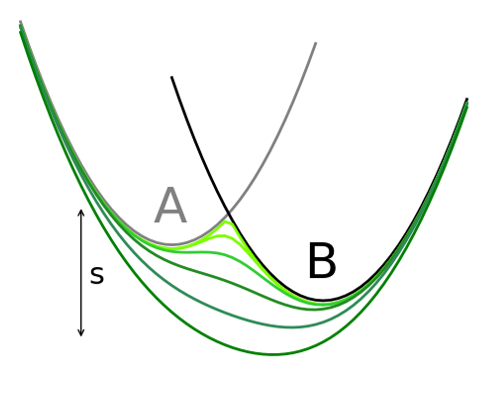
\includegraphics[width=\textwidth]{fig/intro/EDS_parmeters_s.png}
        \caption{Effect of $s$ on $V_R$}
        \label{fig: EDS_potential_behavioura}
    \end{subfigure}
    \begin{subfigure}{0.44\columnwidth}
        \centering
        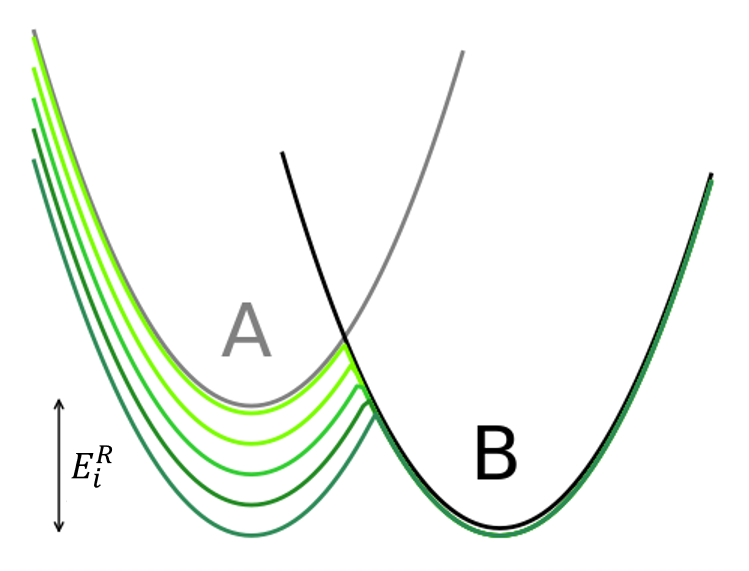
\includegraphics[width=\textwidth]{fig/intro/EDS_parmeters_Eoff.png}
        \caption{Effect of $E_i^R$ on $V_R$}
        \label{fig: EDS_potential_behaviourb}
    \end{subfigure}
    \end{center}
    \caption{Schematic illustration of the effect of the two types of EDS reference-state parameters. (\textbf{A}): The smoothing parameter $s$ decreases the barriers between the end states. If $s$ is too small, an ``undersampling'' situation occurs with a global unphysical minimum. (\textbf{B}): The energy offsets $\textbf{E}^R$ provide equal weighting to all end states in the EDS reference state.  The figure was generated with Ensembler\cite{Ries2021} (Chapter \ref{ch:feens}).}
    \label{fig: EDS_potential_behaviour}
\end{figure}

% laws of motion of R
The force on a particle $k$ in the EDS reference state is calculated as \cite{Christ2008},
\begin{equation}
    \textbf{f}_k(t)=-\frac{\partial V_R(\textbf{r}; s, \textbf{E}^R)}{\partial \textbf{r}_k} = \sum^N_{i=1}\frac{e^{-\beta s(V_i(\textbf{r}) -E_i^R)}}{\sum^N_{j=1}{e^{-\beta s (V_j(\textbf{r})-E_j^R)}}}  \left( -\frac{\partial V_i(\textbf{r})}{\partial \textbf{r}_k} \right) \,.
    \label{eq:laws_of_motion}
\end{equation}
%
For $s$ values close to one, the reference-state forces are dominated by the one end state, for which the current coordinates are most favourable, while the other end states give high energies and therefore contribute little (i.e. ``dummy states'').  
For small $s$ values (undersampling situation), all end states contribute effectively to the forces, resulting in the global unphysical minimum.

%% ddFE
The free-energy difference between two end states $A$ and $B$ can be calculated by employing the Zwanzig equation twice forming a path via the reference state~$R$ \cite{Zwanzig1954,Christ2007,Christ2008},

\begin{align} \nonumber
    \Delta G_{\text{BA}} &=  \Delta G_{\text{BR}} + \Delta G_{\text{RA}} \\ 
    &=-\frac{1}{\beta}\left(\ln \langle e^{-\beta (V_B-V_R)}\rangle_R - \ln \langle e^{-\beta (V_A-V_R )}\rangle_R\right) \\ 
    &= -\frac{1}{\beta} \ln \frac{\langle e^{-\beta (V_B-V_R)}\rangle_R}{\langle e^{-\beta (V_A-V_R)}\rangle_R}.
    \label{EQ: Free Energy calculation via reference state}
 \end{align}

%---------------------------
\FloatBarrier

\subsection{Replica-Exchange EDS (RE-EDS)}
The recently introduced RE-EDS method \cite{Sidler2016,Sidler2017} is a type of Hamiltonian replica exchange \cite{Hansmann1997,Sugita2000} with the smoothness parameter $s$ as the exchange dimension ($1 \geq s > 0$), which was inspired from constant pH simulations by Lee \textit{et al.} \cite{Lee2014,Lee2015}. The approach is shown schematically in Figure \ref{fig:RE-EDS_Scheme}.
RE-EDS does not require a single (optimal) $s$-value. Instead enhanced sampling is achieved by exchanging between the replicas with different smoothness levels. This simplifies the parameter choice problem and thus, the method can be applied to systems with more than two end states \cite{Sidler2016,Sidler2017}.

%Exchange criterium
For the pairwise exchanges between neighboring replicas $k$ and $l$, a Metropolis-Hastings criterion \cite{Hastings1970} is used \cite{Sidler2016,Sugita2000},
\begin{equation}
    \begin{split}
    p_{k,l} = min\bigg(1, \exp \Big[
                &-\beta \big((H_{R}(\textbf{r}_k; s_l)+H_{R}(\textbf{r}_l; s_k))\\
                &-(H_{R}(\textbf{r}_l; s_l)+H_{R}(\textbf{r}_k; s_k))\big)  \Big] \bigg) ,
    \end{split}
\end{equation}
where $H_{R_k}$ and $H_{R_l}$ are the reference-state Hamiltonians of the respective replicas, $\textbf{r}_k$ and $\textbf{r}_l$ are the current coordinates of the replicas.

Replicas are placed between $s=1.0$ and a lower bound of $s$, where the reference state is in undersampling. The replicas with low $s$ values facilitate the transitions between the low-energy regions of the  different end states. Especially for systems with slowly adapting environments (e.g. protein binding pockets), regions in $s$-space with very low acceptance probability can occur. Thus, to ensure sufficient exchanges between all pairs of replicas, a local variant of the round-trip time optimization algorithm \cite{Katzgraber2006, Nadler2008} was developed to optimally place the replicas in $s$-space \cite{Sidler2017}.
It was found that a single set of energy offsets can be used for all replicas \cite{Sidler2016}. However, it is important that these energy offsets are chosen well to avoid ``leakage'' effects, resulting in one or more end states not being properly sampled \cite{Sidler2016}.
The final free-energy differences are estimated from the replica at $s=1.0$, which represents the physical minima of the end states.

\begin{figure}[h]
    \centering
    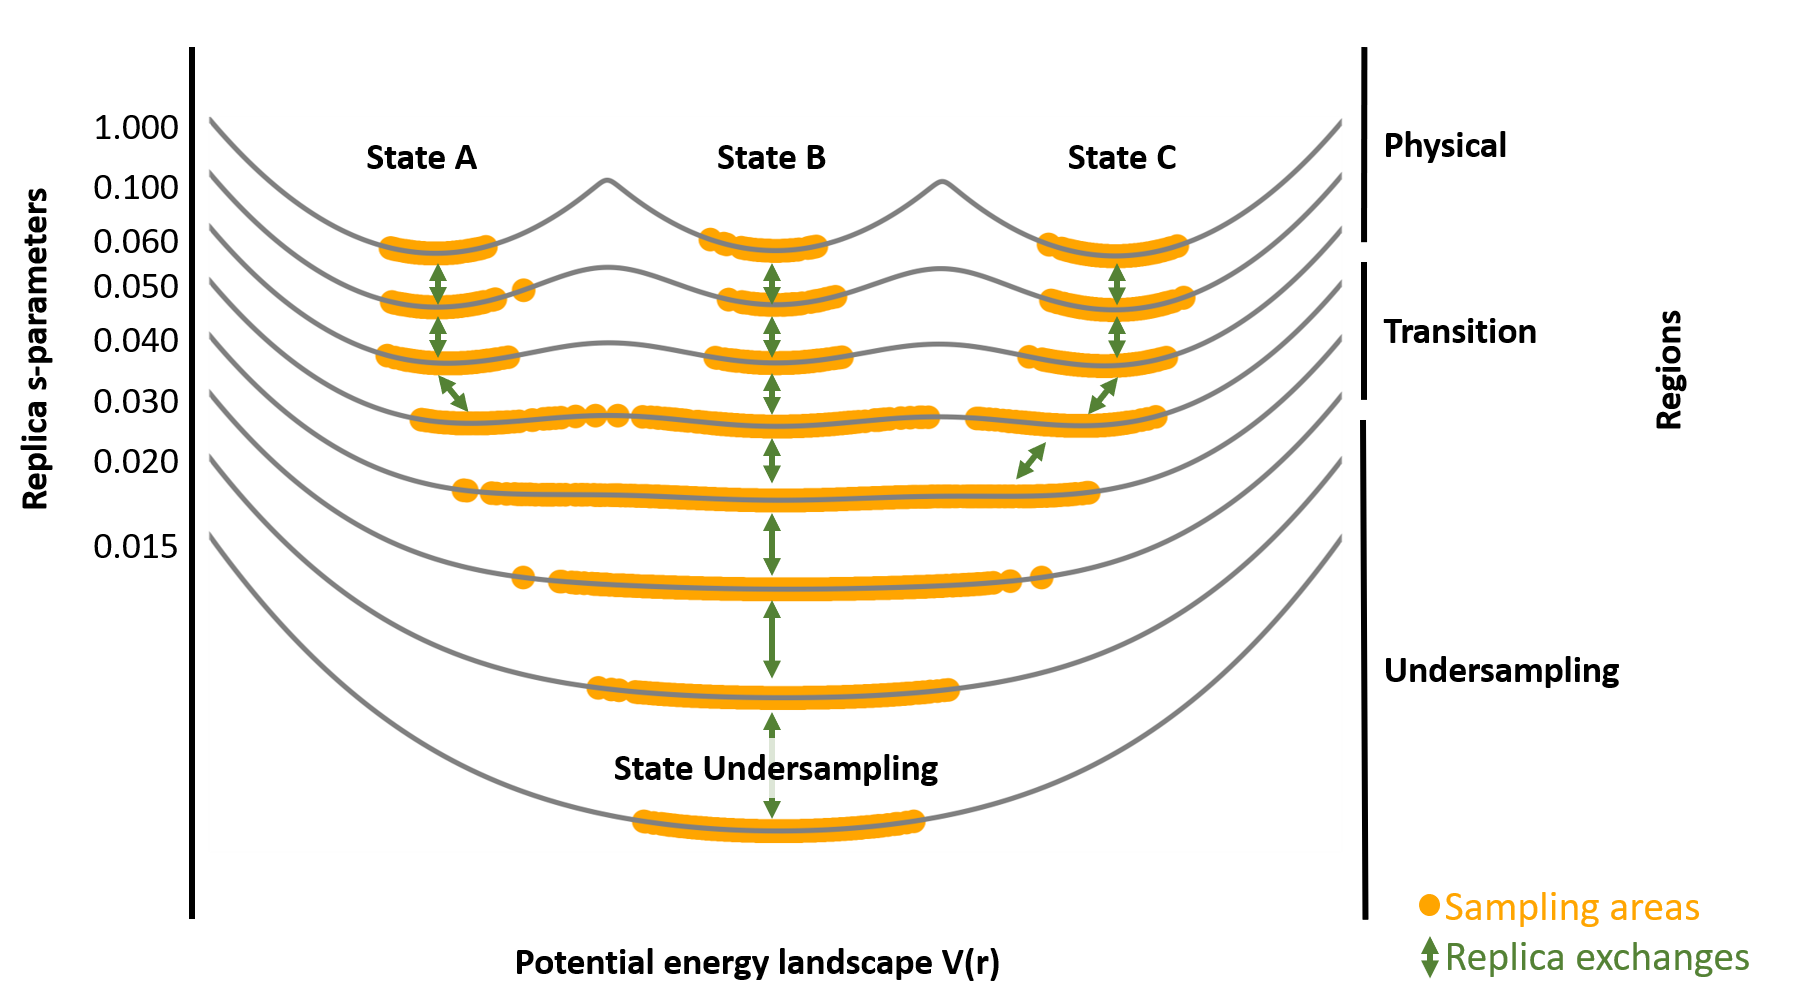
\includegraphics[width=\columnwidth]{fig/theory/Reeds_scheme_first.png}
    \caption{Schematic illustration of RE-EDS with three harmonic oscillators as end states ($A$, $B$, and $C$). Each replica differs by the $s$-parameter, generating reference states with a different degree of smoothness. Sampling of each replica is denoted with orange dots. Exchanges between the replicas are indicated with green arrows. The replica graph shows three regions: a ``physical'' region where $s$ is close to 1, a transition region, and the ``undersampling'' region when $s$ approaches zero. The figure was generated with Ensembler \cite{Ries2021}  (Chapter \ref{ch:feens}).}
    \label{fig:RE-EDS_Scheme}
\end{figure}

%---------------------------
\FloatBarrier

\subsection{Automatic Parameter Optimization}
To facilitate the determination of the energy offsets and $s$-parameter distribution, we have extended and further automatized the previous \cite{Sidler2017} RE-EDS workflow (Figure \ref{fig:Workflow}).
\begin{figure}[h!]
    \centering
    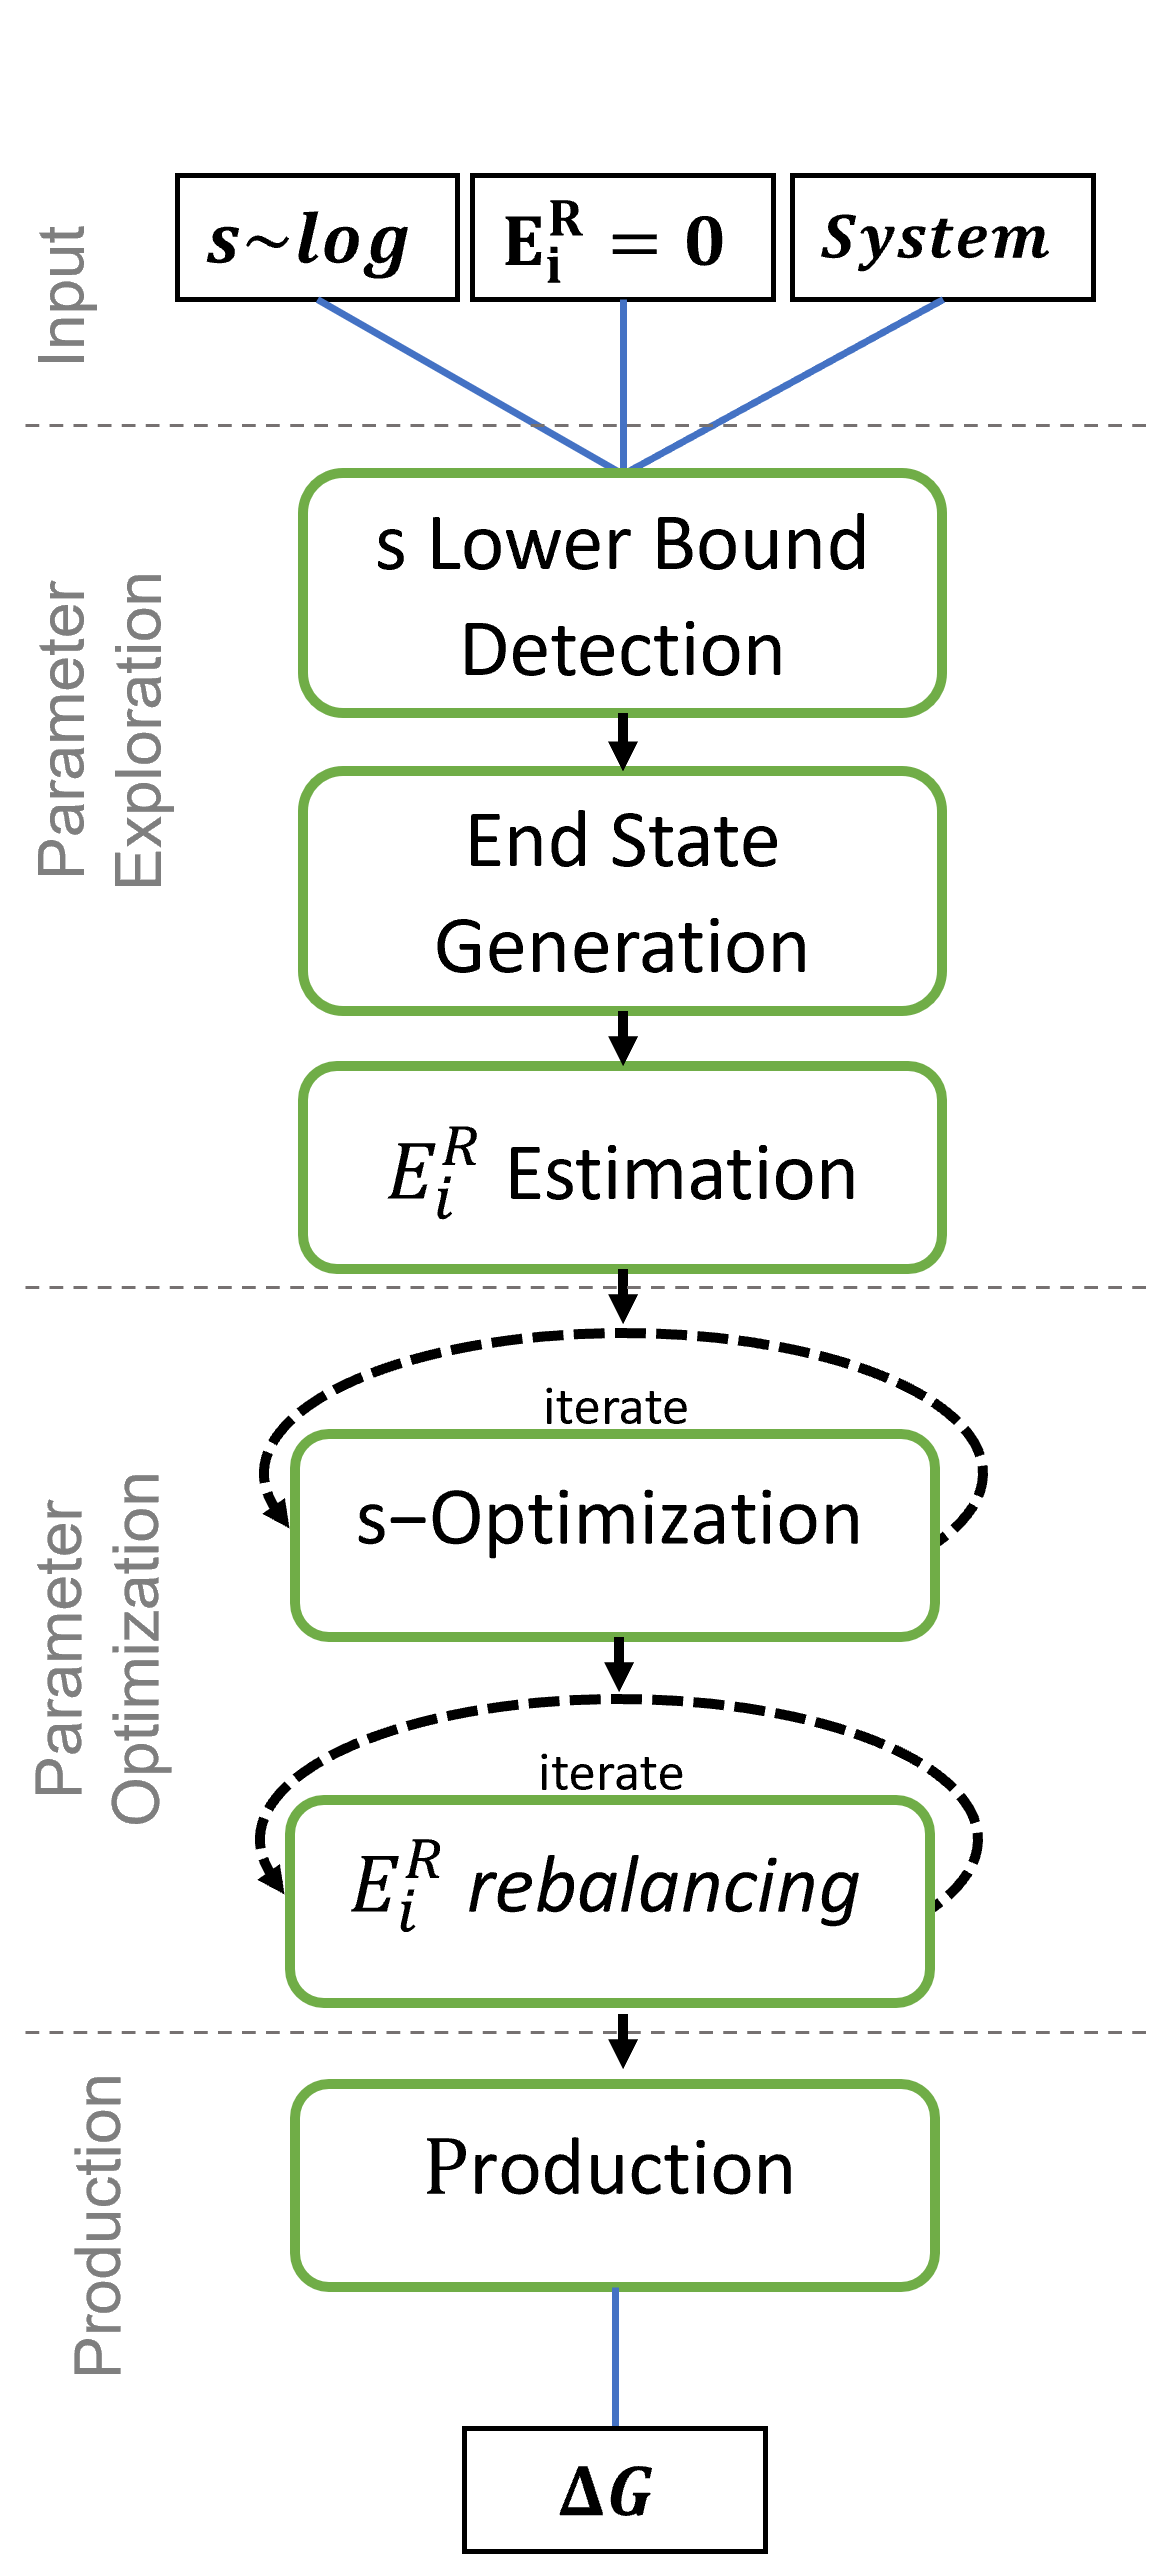
\includegraphics[width=0.5\columnwidth]{fig/theory/RE_EDS_Pipeline.png}
    \caption{The RE-EDS workflow can be split into four steps: (1) Input stage with energy offsets set to $E_i^R=0$ and a set of $s$-parameters logarithmically distributed between $1$ and $10^{-5}$; (2) Parameter exploration to determine the lower bound for $s$, to obtain equilibrated coordinates for each end state, and to estimate initial energy offsets with the PEOE scheme \cite{Sidler2016}; (3) Parameter optimization to improve the $s$-distribution with the N-LRTO algorithm \cite{Sidler2017} and the state sampling with energy offset rebalancing; (4) Production run and calculation of the free-energy differences.}
    \label{fig:Workflow}
\end{figure}

%
The initial input for a system with $N$ end states consists of a prepared EDS system (i.e. topology,  perturbation topology, initial coordinates, and distance restraints), a list of energy offsets of length $N$ with $E_i^R = 0; ~ \forall ~ i \in [1,...,N]$, and a list of $s$-parameters, which are logarithmically distributed in the range $s_i \in [1, 10^{-5}]$. Typically, we use 21 initial $s$ values. 

The parameter exploration consists of three substeps: (i) determining the lower bound for the $s$-distribution (newly introduced), (ii) obtaining optimized coordinates within the EDS set-up for each end state (newly introduced), and (iii) estimation of an initial set of energy offsets (as done previously in Ref.~\citenum{Sidler2016}).

%%1. initial parameter search
To enable sampling of all end states at $s=1.0$, some replicas have to be in undersampling to facilitate transitions. However, for efficiency reasons (and numerical stability) the number of replicas $M$ in undersampling should be small and the lowest $s$-value should be as high as possible. From a short simulation with the initial $s$-distribution between $[1, 10^{-5}]$, the highest smoothing parameter $s_{M_\mathrm{us}}$ at which undersampling still occurs is determined and used in the following as a lower bound for the $s$-distribution. The $s$-distribution for the next step is then defined by logarithmically distributed replicas between $s=1.0$ and the automatically determined lower bound.

%%%state optimization
Optimized coordinates for each end state in the EDS setup can be automatically obtained by short parallel simulations, where one end state in turn is favoured by setting an arbitrarily large energy offset for this state. 
The optimized coordinates allow the user to start RE-EDS simulations from different end states and are needed for the subsequent parameter optimization. 

 %%% estimate EOFFs:
In the last substep, $E_{\text{i}}^{\text{R}}$ estimation, the previously developed parallel energy offset estimation (PEOE) \cite{Sidler2016} scheme is used to estimate the initial set of energy offsets. This is done based on a short simulation with the initial parameters. For each replica $k$ in the undersampling region, the energy offsets are extracted using \cite{Sidler2016},
\begin{equation}
    E_{i}^{R}(new)=-\frac{1}{\beta}\ln \Big < e^{-\beta \big(V_i(\textbf{r})-V_R(\textbf{r}; s_{k},\textbf{E}^{R}(old))\big)}\Big>_{R(s_{k},\textbf{E}^{R}(old))} .
    \label{eq: EoffEstimator}
\end{equation}
The energy offsets that were extracted in parallel for the $k$ replicas are subsequently averaged and used as initial set of energy offsets. These energy offsets should provide a first solution that is close to the optimal choice of energy offsets, which leads to an optimal state sampling of all end states in the RE-EDS simulation. As the initial energy offsets are obtained from the replicas in undersampling, they may not be exactly optimal and require fine-tuning in the next phase. 


%%2. optimization of parameters
In the second step of the RE-EDS workflow, first the $s$-distribution is optimized and subsequently the energy offsets are fine tuned.
%
%%% s-Optimization:
The $s$-distribution is improved by minimizing the round-trip time $\tau$ and increasing the number of round-trips, using the multistate local round-trip time optimization (N-LRTO) algorithm \cite{Sidler2017}. The optimization is performed in an iterative manner with short simulations.
This step is required as exchange bottlenecks between two replicas might occur leading to a very slow round trip time or to no round trips at all. 
In the N-LRTO algorithm, new replicas are inserted in each iteration by linear interpolation in the $s$-regions with exchange bottlenecks, while the replica positions of the previous iteration are retained. Adding replicas theoretically increases the round-trip time because of a longer path between the top and bottom replicas. However, the addition of intermediate replicas also increases the exchange probability between neighboring replicas, thus reducing the round-trip time. With the optimization algorithm, we aim to determine the balance between the length of the replica path and the likelihood of exchange between replicas for minimal round-trip time. The exchange bottlenecks are identified for each end state separately (i.e. multistate). The number of replicas added can be chosen by the user. The iteration is stopped when the average round-trip time $\overline{\tau}$ converges. 
The N-LRTO variant is needed for systems for which severe bottlenecks are observed with the initial logarithmic $s$-distribution (e.g. protein binding pockets). For systems with smaller perturbations, the global multistate variant (N-GRTO) \cite{Sidler2017} can be more efficient as this algorithm re-distributes the replicas in $s$-space according to the exchange statistics. %In very severe cases, this can lead to an oscillating behavior, as one bottleneck is fixed, but another appears due to an imbalance of replica shifting.
%
In this study, we started with the same number of replicas as used for the PEOE scheme above and added four replica positions per iteration in the N-LRTO algorithm.

%%%% Eoff Rebalancing:
After optimizing the number of round trips and $\tau$, the distribution of the state sampling is improved. To reach the ideal situation that each end state is sampled to an equal amount, the initial energy offsets need to be fine tuned, while keeping the round trips approximately constant. For this, we introduce here the energy offset rebalancing scheme.
To avoid overshooting, a correction factor is calculated and applied iteratively,
\begin{equation}
    \Delta E^{corr}_i = - \frac{1}{\beta} \ln \left( \frac{f_i^{\text{mc}}+c}{f^{\text{mc,ideal}}_{i}+c} \right),
    \label{eq: EoffRebalancing}
\end{equation}
where $f_i^{\text{mc}}$ is the current sampling fraction (or estimated probability) of an end state contributing to $V_R $, and $f^{\text{mc,ideal}}$ is the ideal sampling fraction (see Section \ref{metrics}). 
%
To make the approach more robust, a pseudo count $c$ is introduced to avoid singularities with zero sampling, which is defined as,
\begin{equation}
    c = \frac{f^{\text{mc,ideal}}}{x},
    \label{eq: EoffRebalancingPseudoCount}
\end{equation}
with the intensity factor $x$.
The default of the pseudo count was chosen to result in a maximal correction of $\Delta E^{corr}_i=8.43$~kJ/mol, corresponding to a minimum 30-fold reduced sampling compared to the expected optimal sampling.

%%% 3. production run
After optimizing the RE-EDS parameters, the production run is performed for a chosen length. 
The free-energy differences are subsequently calculated using the replica at $s=1.0$ with Eq.~(\ref{EQ: Free Energy calculation via reference state}).

\subsubsection{Starting State Mixing}
The sampling in RE-EDS simulations can be further improved by using starting coordinates for the replicas corresponding to the different end states (i.e. replica 1 starts in a low-energy configuration for end state 1, replica 2 in a low-energy configuration for end state 2, etc.). This technical approach is called ``starting state mixing'' (SSM) in the following and is also used for Hamiltonian replica-exchange TI calculations (see e.g. \citenum{Graf2016, Hahn2020}). The optimized coordinates obtained in the parameter exploration step can be used for SSM. We compare RE-EDS simulations with SSM and with a single set of starting coordinates (abbreviated as 1SS).  

\subsubsection{Analysis}
\label{metrics}
Three types of metrics were used to quantify the sampling in RE-EDS simulations. The first metric determines for each end state $i$ the sampling fraction where it is maximally contributing to the reference state, i.e. $f_i^{\text{mc}}$. A maximally contributing state is defined as the end state with the lowest potential energy minus its energy offset in a frame. As can be seen in  Eq.~\eqref{eq:laws_of_motion}, maximally contributing end states have the largest impact on the reference-state sampling at a given time point.

%
Optimal sampling in a RE-EDS system is achieved when all end states are sampled as maximally contributing states to an equal extent at $s=1.0$, i.e. 
\begin{equation}
f_{i}^{\text{mc,ideal}} = \frac{1}{N} ~, \forall ~ i~\in~ \{1, ..., N\}
\label{eq: optimalDominationSamplingDist}
\end{equation}

The second metric is the estimated sampling fraction of ``physical occurrence'' of an end state $i$, i.e. $f_i^{\text{occur}}$. As a result of phase-space overlap with the current maximal contributing end state, other end states in the EDS system might be sampled simultaneously. An end state is counted as ``occurred'' when its potential energy is below the threshold $V_i \leq T_{i}^{\text{phys}}$ at a time point $t$. 
These thresholds are estimated during the second substep of the parameter exploration phase. If end states show no phase-space overlap, $f_i^{\text{occur}}$ will be (nearly) the same as $f_i^{\text{mc}}$. 

Undersampling is detected with a third metric using the thresholds $T_{i}^{\text{us}}$. These thresholds are determined in the first substep of the parameter exploration phase from the simulation with the lowest $s$-value. If all end states have a potential energy below their respective $V_i - E^R_i \leq T_{i}^{\text{us}}$, the current frame is characterized as undersampling. \cite{Sidler2016} 

\FloatBarrier

%================================================================================
\section{Computational Details}
%================================================================================

In the computational studies, two pairs of structurally similar cyclic peptides were selected, i.e., Nleu-5R/Nleu-5S and Nleu-2R/Nleu-2S (Figure \ref{fig:permCMols}). 
The first pair presents a ``permeability cliff'', i.e., the two peptides show a large difference in the passive permeability in the PAMPA assay (Nleu-5R: $−log(P_e)$~=~5.4; Nleu-5S: $−log(P_e)$~=~7.2), despite a high structural similarity. 
In contrast, the second pair is similar in both structure and permeability (Nleu-2R: $−log(P_e)$~=~6.1; Nleu-2S: $−log(P_e)$~=~5.8). 
For each of these four peptides, $250$ starting coordinates were generated using the macrocycle variant of the OMEGA conformer generator from OpenEye. \cite{Hawkins2012, Hawkins2010, Poongavanam2018}
Conformers were energy-minimized for maximum $2000$ steps with the steepest descent \cite{Ruder2016} approach using the GROMOS software package \cite{Schmid2012} with the GROMOS 54A7 force field. \cite{Schmid2011} 
Each minimized starting conformation was solvated in a cubic box of simple-point-charge (SPC) water \cite{Berendsen1981} (on average, $4172$ solvent molecules) or chloroform \cite{Tironi1994} (on average, $980$ solvent molecules). 
For each system, an MD simulation of $101~$ns length was performed under isothermal–isobaric (NPT) conditions with the leap-frog integration algorithm \cite{Hockney1970, Gunsteren1988} and a time step of $2$~fs. 
The first 1 ns was discarded as equilibration. Bond lengths were constrained with SHAKE \cite{Ryckaert1977} and a tolerance of $10^{–4}$~nm. 
Nonbonded interactions were calculated using a twin-range scheme with a short-range cutoff of $0.8$~nm and a long-range cutoff of $1.4$~nm. 
The electrostatic nonbonded contributions beyond the long-range cutoff were calculated with the reaction-field \cite{Tironi1995} approach, setting the dielectric permittivity to 61.0 \cite{Heinz2001} for water, and to 4.8 \cite{Tironi1994} for chloroform. 
The temperature was kept constant at $300$~K using the weak coupling scheme \cite{Berendsen1984} and a coupling time of $0.1~\text{ps}^{–1}$. 
The pressure was kept at $1.031$~bar ($1$~atm) with the same type of algorithm, a coupling time of $0.5~\text{ps}^{–1}$, and an isothermal compressibility of $0.001654~\text{bar}^{–1}$ for chloroform and $0.0004575~\text{bar}^{–1}$ for water. 
Translational motion of the center of mass of the simulation box was removed every $2$~ps. Energies and coordinates were written every $5$~ps.

Trajectory analysis was performed with PyEmma \cite{Scherer2015} and MDTraj \cite{Mcgibbon2015}. 
The selection of features for the structural clustering consisted of the distances between all pairs of polar atoms and the backbone torsional angles, resulting in total $57$ features. 
This selection was reduced to three to five dimensions (depending on the peptide) with TICA \cite{Molgedey1994} using a cumulative variance of $0.9$ as criterion and a TICA correlation lag time of $50$~ps. 
Based on these TICs, the frames were clustered with a common nearest neighbor (CNN) algorithm \cite{Keller2010, Weiß2021} using a cutoff of $0.2$ and a similarity of $20$. 
Comparison of selected clusters with NMR experiments was performed with the GROMOS++ package of programs. \cite{Eichenberger2011}
The coefficients for the Karplus curve were taken from Vögeli \textit{et al.} \cite{Voegeli2015}
Analysis of hydrogen bonds and torsional angles was performed with MDTraj. 
The 3D-PSA was calculated with our implementation \cite{Witek2019} of the workflow in Ref.~\citenum{Tyagi2018} using PyMol \cite{Delano2020}.
Statistical analysis of all results was carried out using the Python packages Pandas, NumPy and SciPy.\cite{Virtanen2020}



%================================================================================
\section{Results and Discussion}
%================================================================================

The chosen model system of five inhibitors of CHK1 kinase exemplifies different core-hopping transformations (i.e. ring size change, ring opening/closing, ring extension) and R-group modifications \cite{Wang2017}, increasing the complexity compared to the systems previously studied with RE-EDS. Furthermore, the performance can be directly compared to the results obtained with FEP+ and OPLS3 in Ref.~\cite{Wang2017} as well as with QligFEP results in Ref.~\cite{Jespers2019}.

\subsubsection{Parameter Exploration and Parameter Optimization}
The RE-EDS workflow was started by estimating the lower bound for the $s$-distribution. Using the above mentioned undersampling criterion (see Methods section), a lower bound of $s=0.01$ was determined for the protein-ligands complex and $s=0.0056$ for the ligands in water. 

%State Optimizations
Optimized coordinates were obtained for all five ligands, as verified by comparing the potential-energy distribution from the EDS simulation with the one extracted from a standard MD simulation of the respective ligand (Figure S1 in the Supporting Information). % SUPPL
From these same steps, the potential-energy thresholds for the occurrence sampling ($T_{i}^{\text{phys}}$) and undersampling ($T_{i}^{\text{us}}$) were estimated.

%Eoff:
The energy offsets $\vec{E}^R$ were estimated from a short RE-EDS simulation with the PEOE \cite{Sidler2016} scheme and are listed in Table \ref{tab:CHK1_set2_Eoff}.
For $s=1.0$, the energy offsets should ideally be equal to the free energy of the corresponding state (i.e. $\Delta E^R_{ji} = \Delta G_{ji}$) such that the partition function of the reference state is the sum of the partition functions of the end states \cite{Christ2008}. Therefore, the comparison between the relative estimated energy offsets in water and in complex ($\Delta \Delta E^R_{ji} = \Delta E^R_{ji,\text{complex}} - \Delta E^R_{ji,\text{water}}$) and the relative binding free energy $\Delta \Delta G^\text{bind}_{ji}$ can be used to (roughly) assess the quality of the estimated energy offsets. As shown in Figure S2 in the Supporting Information, % SUPPL
the energy offsets estimated from the SSM simulations are in better agreement with the experimental relative binding free energies than those estimated from the 1SS simulations.

\begin{table}[h]
\caption{Energy offsets $\vec{E^R}$ estimated from a short RE-EDS simulation using the PEOE \cite{Sidler2016} scheme. The errors indicate the standard deviation over the different replicas in undersampling. All energy offsets were calculated relative to ligand L1. The starting coordinates were selected following the 1SS or the SSM approach (see Theory and Methods sections).}
\label{tab:CHK1_set2_Eoff}
\resizebox{\columnwidth}{!}{%
\centering
\begin{tabular}{ l | r r | r r }
 Ligand & \multicolumn{2}{c|}{Water}&\multicolumn{2}{c}{Complex}  \\ 
  &RE-EDS 1SS [kJ~mol$^{-1}$]&RE-EDS SSM [kJ~mol$^{-1}$]&RE-EDS 1SS [kJ~mol$^{-1}$]&RE-EDS SSM [kJ~mol$^{-1}$]\\ 
 \hline
     L1 & $0.0$ & $0.0$ & $0.0$ & $0.0$ \\ 
     L17 & $11.07 \pm 7.61 $ & $17.81 \pm 0.69 $ & $20.03 \pm 5.04 $ & $18.19 \pm 3.43$ \\
     L19 & $-9.38 \pm 6.85 $ & $ -12.37 \pm 5.23 $ & $-2.09 \pm 1.56 $ & $ 2.4 \pm 1.56$ \\
     L20 & $-53.15 \pm 2.95 $ & $ -56.01 \pm 13.67 $ & $ -58.73 \pm 4.87 $ & $-52.2 \pm 2.6$\\
     L21 & $-76.75 \pm 5.79 $& $-69.15 \pm 3.74 $ & $ -77.29 \pm 3.12 $ & $ -77.9 \pm 3.4$\\
\end{tabular}
}
\end{table}

%S-Optimization
The optimization of the $s$-distribution was performed with the N-LRTO \cite{Sidler2017} algorithm, thereby minimizing the average round-trip time $\overline{\tau}$ in the replica graph. For the 1SS complex system, four optimization iterations were used. For the other systems, three iterations were used. 

%
In the first iteration, the total number of observed round trips was very low or zero for all approaches. In the following iterations, this quantity increased, and the average round-trip time decreased for all simulations (Figure \ref{fig: CHK1_RingOpening_sOptimization}). The number of round trips was generally smaller in the complex than in water due to a more pronounced gap region \cite{Sidler2017}.
Already after the second iteration, the round-trip time was reduced in all approaches. The improvement of the $\overline{\tau}$ over the iterations can also be seen in Figure S3 in the Supporting Information. % SUPPL
%% s-replica placements
As can be seen in the third row of Figure \ref{fig: CHK1_RingOpening_sOptimization}, the optimization algorithm increases the density of the replicas around $s = 0.041$, where the major gap region lies.

\begin{figure}[h]
\centering
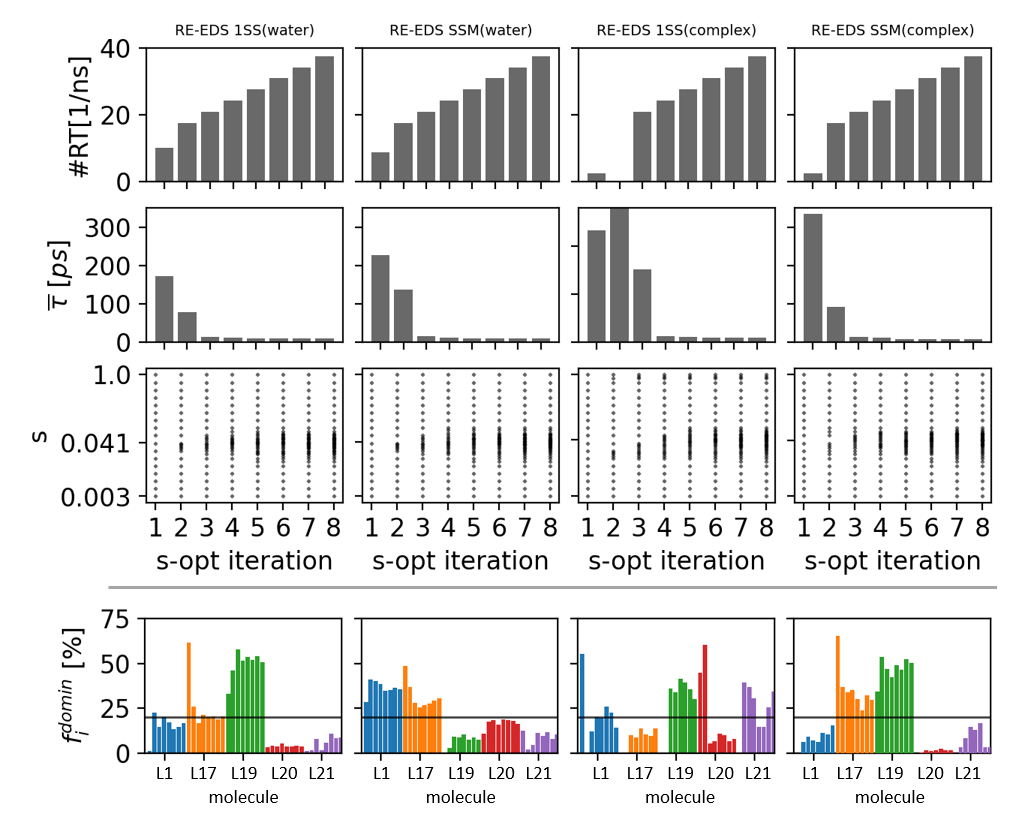
\includegraphics[width=\textwidth]{fig/results/ringOpening/paramOptimization/S-optimization_ringOpening.png}
\caption{Optimization steps of the $s$-distribution with the N-LRTO \cite{Sidler2017} algorithm followed by the energy offset rebalancing scheme (start indicated by the red horizontal line). The measured quality criteria were the number of round trips (1. row), the average round-trip time $\overline{\tau}$ (2. row), the placement of the replicas in $s$-space (3. row), and the sampling fractions of maximally contributing states $f_{i}^{\text{mc}}$ (4. row). The light colored bars of $f_{i}^{\text{mc}}$ indicate $s$-optimization iterations, whereas the fully colored bars indicate energy offset rebalancing steps. }
\label{fig: CHK1_RingOpening_sOptimization}
\end{figure}



%% tau converge - Conclusion
The $s$-optimization was stopped after a sufficiently high number of round trips and low round-trip time was reached. 
This resulted in 20 replicas for the ligands in water after three $s$-optimization iterations.
For the protein-ligands complex, the fourth $s$-optimization iteration was chosen for the 1SS approach, and the third iteration for the SSM approach, resulting in 29 and 25 replicas, respectively. 
The average round-trip time after convergence was $\overline{\tau} = 0.4 \pm 0.2$~ns for all simulations.

After the $s$-optimization, the energy offset rebalancing scheme was applied to improve the state sampling. 

%RT analysis
During the rebalancing steps, no further replicas were added to the $s$-distribution. It is essential for the success of the rebalancing scheme that round trips occur. Therefore, the number of round trips and average round-trip time were monitored. In all systems, the number of round trips and $\overline{\tau}$ remained relatively stable over the four rebalancing steps. For the RE-EDS 1SS approach in water, the number of round trips slightly decreased but never dropped to zero.

%% states sampling
Across the optimization steps, also the sampling of the end states as maximally contributing states at $s=1.0$ was monitored.
During the $s$-optimization, some end states ``vanish'' and are no longer sampled as maximal contributing states. This leakage effect can occur when the initially estimated $E^{\text{R}}$ are not exactly optimal \cite{Sidler2016}. 
With energy offset rebalancing, the sampling of each end state can be recovered, and the sampling distribution approaches the ideal case.
%After the s-optimization the MAE($P^{\text{maxContrib}}$) was for all approaches approximately at $25\%$, with the exception of the 1SS water system, here it was $20\%$. 
After rebalancing, all end states showed a $f_i^{\text{mc}} > 0$ and the mean absolute deviation of the sampling distribution from ideal decreased from $20-25\%$ to approximately $7-12\%$ (Figure S4 in the Supporting Information). % SUPPL
 
\subsection{Free-Energy Calculation}
After successfully optimizing the RE-EDS parameters, the production runs were performed for $3.5$~ns. 

%%Sampling++
Both in water and in complex, the potential-energy distributions of the end states generally match well the corresponding distributions from the standard MD simulations of the single end states (Figure \ref{fig:RingOpening_sampling_comparison}). Only in the complex 1SS approach, a deviation can be seen for L17, with a slight shift to higher potential energies. This is due to insufficient sampling of L17 in this case (see below). 
%
The analysis of the maximally contributing end states at $s=1.0$ shows that in water all end states were sampled close to the ideal equal distribution (Figure S5 in the Supporting Information). % SUPPL
In the simulation of the protein-ligands complex, there are still differences in sampling. Especially with the 1SS approach, L19 is generally sampled too much, while L17 is not sampled enough. The situation is improved with the SSM approach.
Comparing $f_i^{\text{occur}}$ and $f_i^{\text{mc}}$ in Figure S5 indicates that the end states in the CHK1 system are clearly separated (i.e. no phase-space overlap). % SUPPL

\begin{figure}[h]
    \centering
    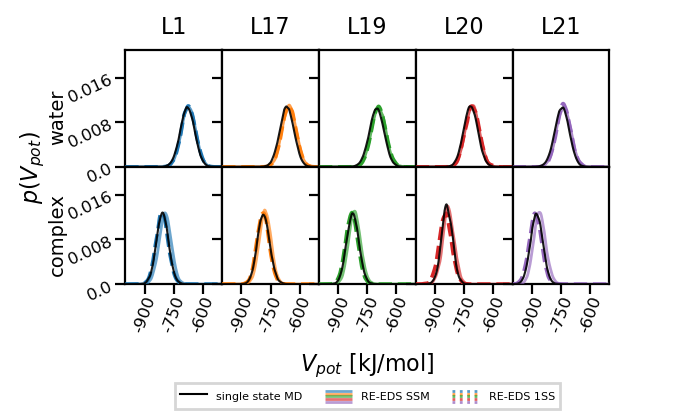
\includegraphics[width=\columnwidth]{fig/results/ringOpening/FE/RingClosure_system_final_sampling.png}
    \caption{Comparison of the Boltzmann reweighted potential-energy distributions obtained from standard MD simulations of a given end state (black) and from the RE-EDS production runs of the 1SS (green) and SSM (turquoise, dashed) approaches.}
    \label{fig:RingOpening_sampling_comparison}
\end{figure}

%%Accuracy
From the replica at $s=1.0$, the free-energy differences were calculated using Eq.~(\ref{EQ: Free Energy calculation via reference state}) and the resulting $\Delta \Delta G^\text{bind}_{ji}$ were compared with the experimental results taken from Ref.~\cite{Huang2012}. The results are shown graphically in Figure \ref{fig:CHK1_set2_FreeEnergyCalculation} and numerically in Table \ref{tab: RE-EDS_FE_RingCycleOpening_ddF}. The individual free-energy differences are given in Table S3 in the Supporting Information. %SUPPL
The RMSE with RE-EDS 1SS is $4.4$~kJ~mol$^{-1}$ and the MAE is $3.9\pm2.8$~kJ~mol$^{-1}$. 
%
%how I calculate the MAE and RMSD:
%MAE = np.mean(np.abs(ddG_differences))
%std(MAE) = np.std(np.abs(ddG_differences)) #gives an impression of absolute deviation of all ddG_diffs
%RMSE = np.sqrt(np.mean(np.square(ddG_differences))
%
The main deviations stem from ligand L17 in the RE-EDS 1SS approach, which can be explained by the insufficient sampling of L17 in the complex (see Figure \ref{fig:RingOpening_sampling_comparison} and Figure S5 in the Supporting Information). %SUPPL

The performance was substantially improved using the SSM approach with RE-EDS, giving an RMSE of $3.3$~kJ~mol$^{-1}$ and an MAE of $2.8 \pm 1.7$~kJ~mol$^{-1}$. 
Only two values (L21-L11) and (L21-L19) deviate more than $4.184$~kJ~mol$^{-1}$ (i.e. $1$~kcal~mol$^{-1}$) from experiment.
The Spearman correlation coefficient for RE-EDS 1SS is $r_{\text{Spearman}}=0.01$ and for RE-EDS SSM $r_{\text{Spearman}}=0.69$.

%%Performance:
Next, we assessed the convergence of the $\Delta G_{ji}$ values as a function of simulation time (Figure S6 in the Supporting Information). % SUPPL
For the RE-EDS 1SS approach, all free-energy differences appeared converged after $2.5$~ns in water and after $2.7$~ns in the complex. For the RE-EDS SSM approach, convergence was observed after $2.5$~ns in water and after $2.9$~ns in the complex.

\begin{figure}[h]
    \centering
    \begin{subfigure}{0.85\columnwidth}
        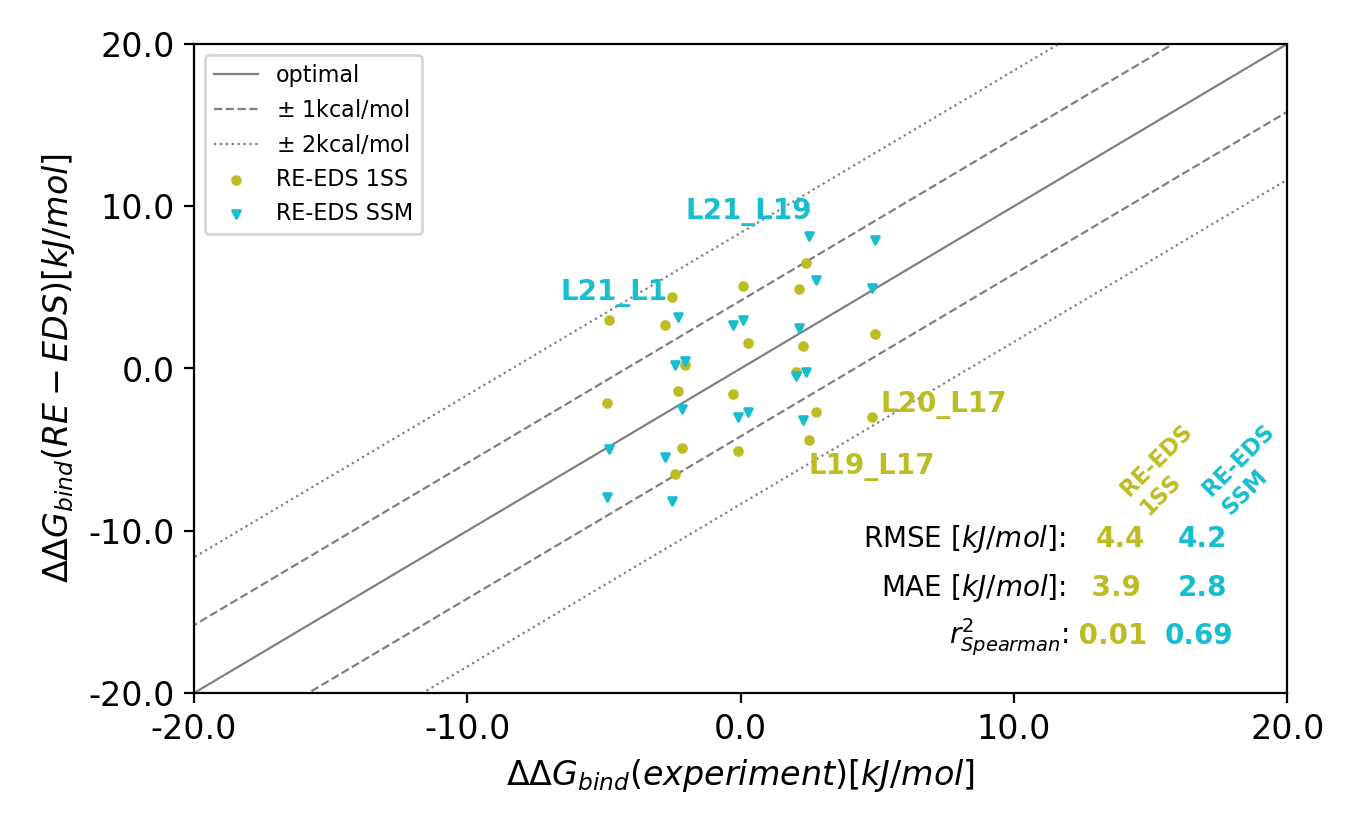
\includegraphics[width=\textwidth]{fig/results/ringOpening/FE/RingClosure_system_final_results_4ns_comparison.png}
        \end{subfigure}
    \begin{subfigure}{0.85\columnwidth}
        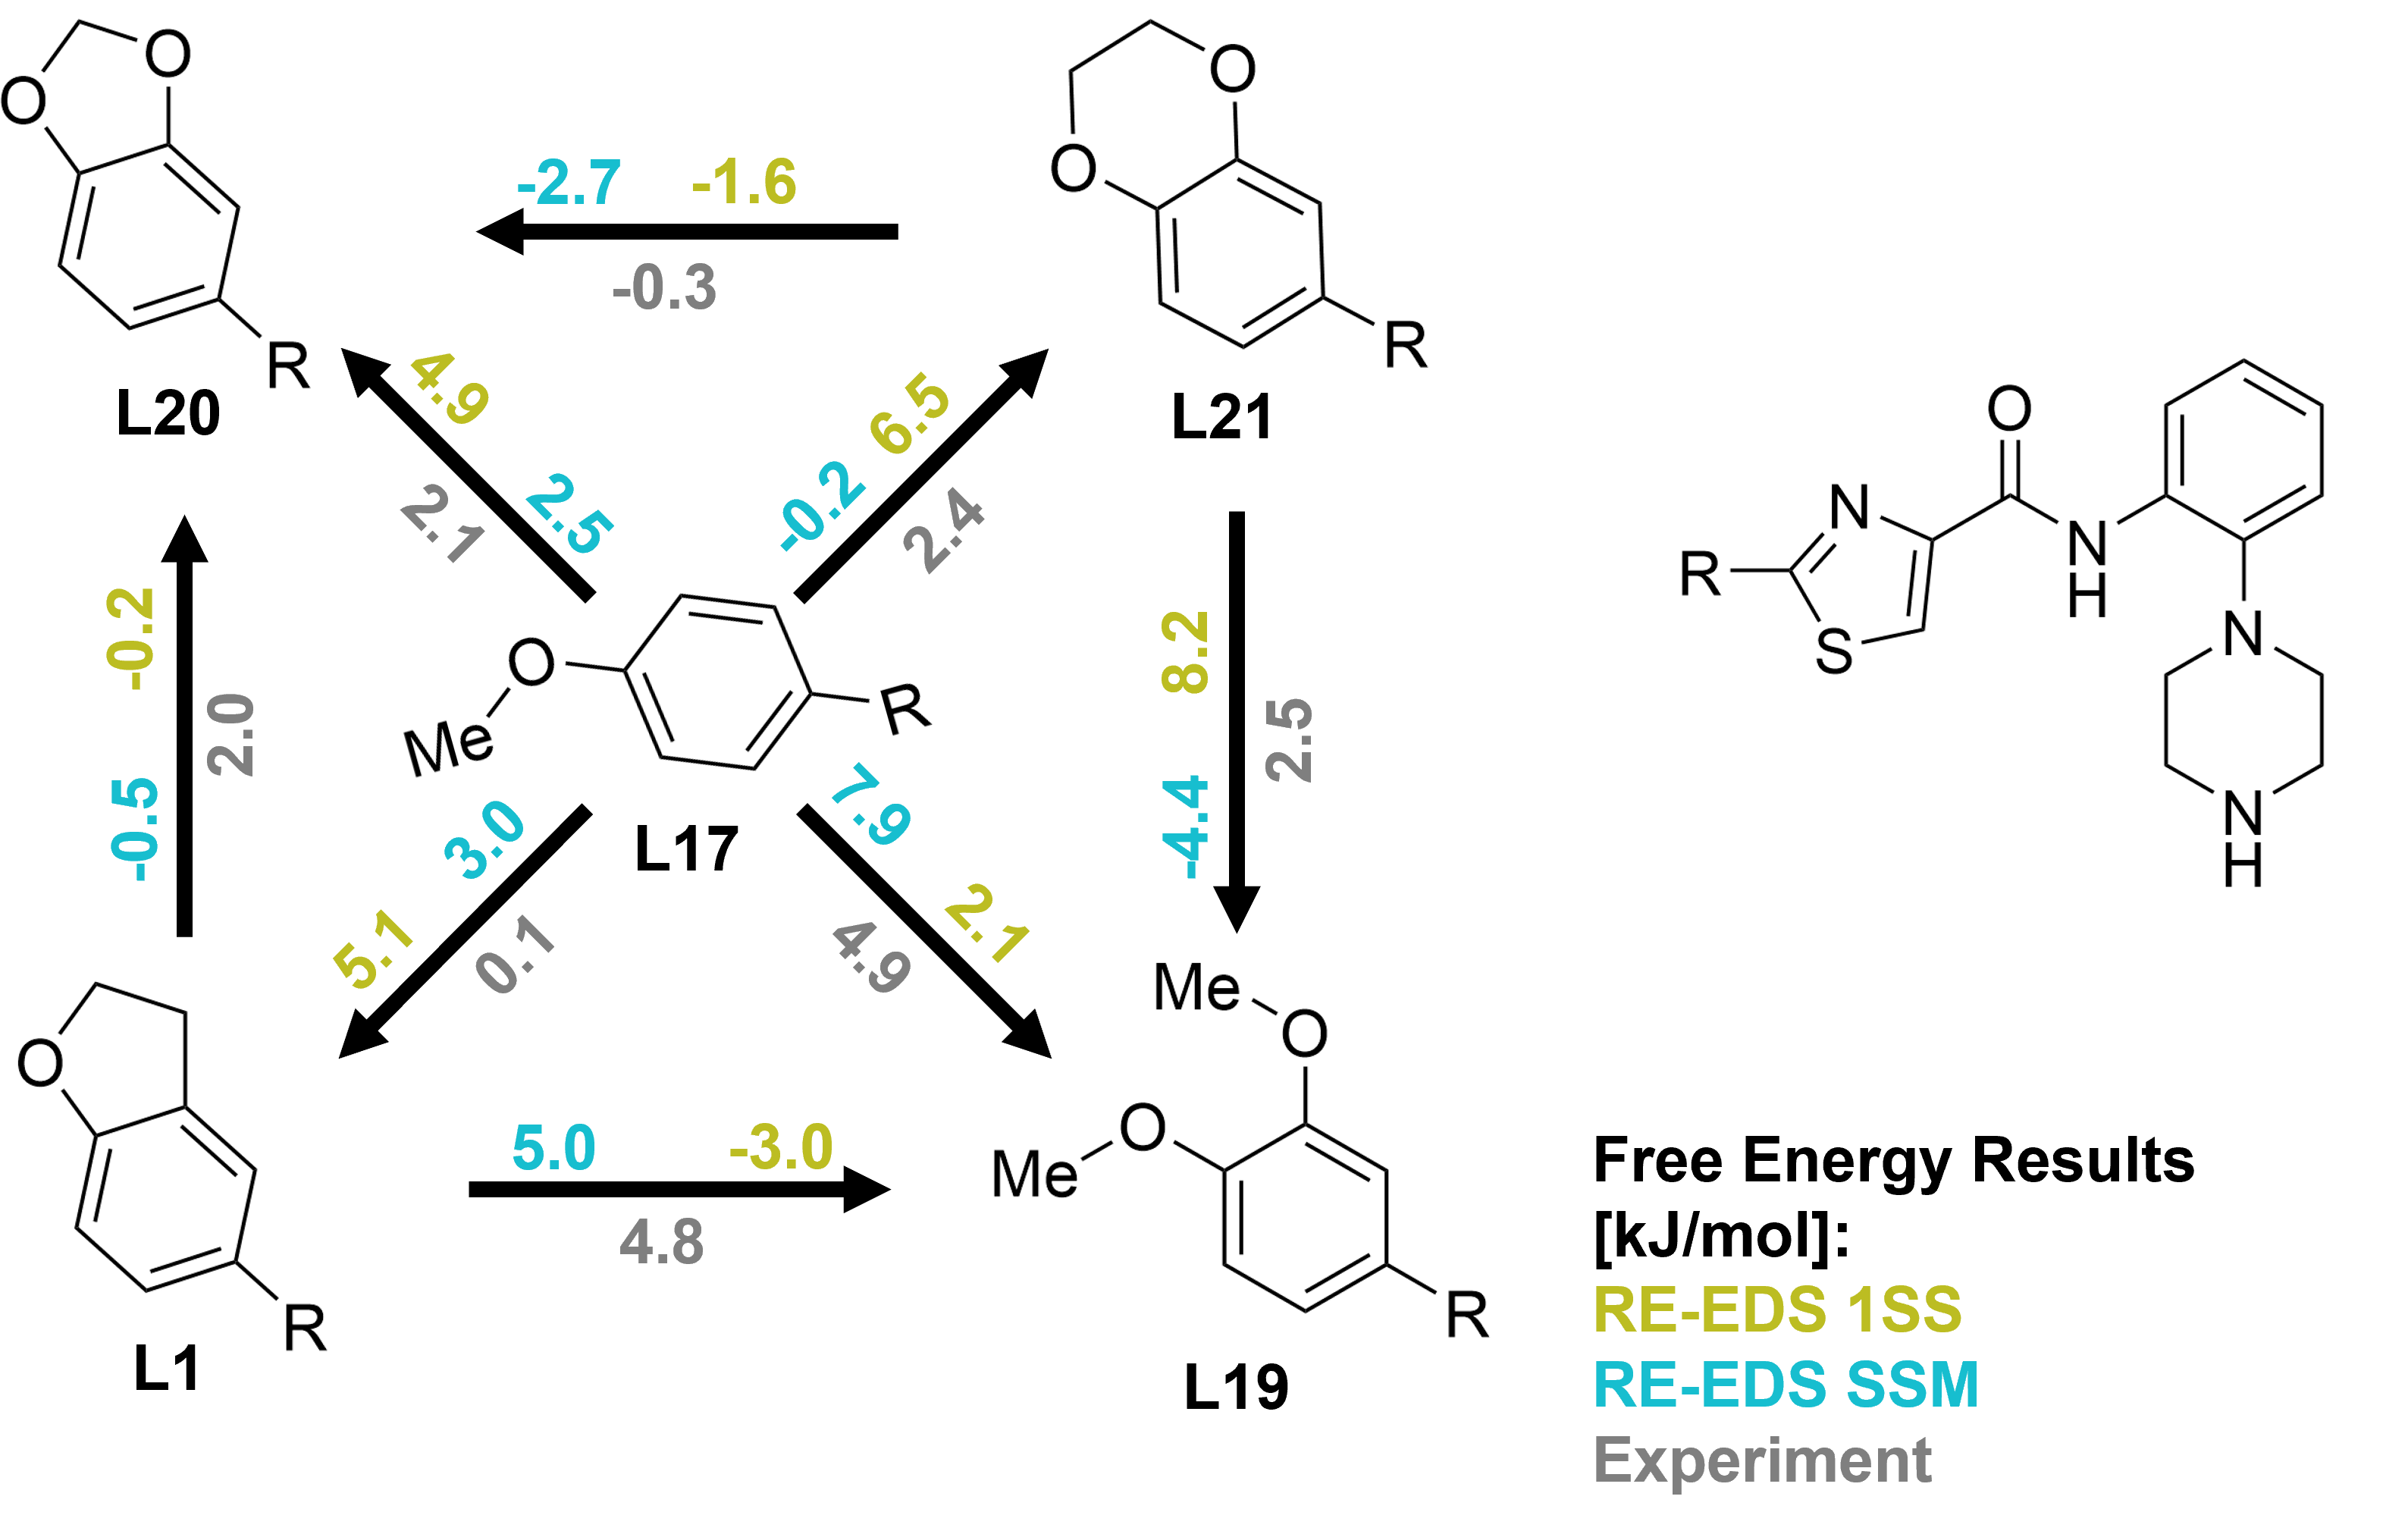
\includegraphics[width=\textwidth]{fig/results/ringOpening/FE/ddG_bind_paper_comparison_reeds_only_4nsSimulation.png}
        \end{subfigure}
    \caption{Free-energy differences estimated from the production run of $3.5$~ns length. (Top): Comparison between the experimental and calculated $\Delta \Delta G^\text{bind}_{ji}$ using RE-EDS 1SS and RE-EDS SSM. The results were calculated with all possible pairwise transformations (forward and backward). (Bottom): Graphical representation of the $\Delta \Delta G^\text{bind}_{ji}$ results with structures, inspired by the one in Ref.~\cite{Wang2017}.}
    \label{fig:CHK1_set2_FreeEnergyCalculation}
\end{figure}

%Comparison results with Schroedinger & Jespers
By applying the RE-EDS methodology to the same system of five CHK1 inhibitors as studied by Wang \textit{et. al.} \cite{Wang2017} and later on also Jespers \textit{et al.} \cite{Jespers2019}, a direct comparison with FEP+ and QligFEP is possible (Table \ref{tab: RE-EDS_FE_RingCycleOpening_ddF}). Note that the quality metrics were calculated over all possible pairs of ligands and in both directions, not only those directly calculated by FEP+ and QligFEP.
For FEP+, we obtained an RMSE of $2.4$~kJ~mol$^{-1}$ and an MAE of $1.8 \pm 1.2$~kJ~mol$^{-1}$ with a Spearman correlation coefficient of $r_{\text{Spearman}}=0.67$.
Including cycle closure correction (CC) \cite{Wang2017} reduced the RMSE to $2.1$~kJ~mol$^{-1}$ and the MAE to $1.9 \pm 1.0$~kJ~mol$^{-1}$. The Spearman correlation coefficient increased to $r_{\text{Spearman}}=0.73$.
Jespers \textit{et al.} \cite{Jespers2019} reported free-energy differences with QligFEP as an average over ten independent replicas, each with significantly less simulation time per $\lambda$-window than in Ref.~\cite{Wang2017}. For QligFEP, an RMSE of $2.3$~kJ~mol$^{-1}$, an MAE of $2.0 \pm 1.2$~kJ~mol$^{-1}$, and a Spearman coefficient of $r_{\text{Spearman}}=0.61$ was obtained.

Overall, the performance of RE-EDS SSM is comparable with the pairwise methods. The results with FEP+ CC and QligFEP showed a slightly higher accuracy compared to experiment, likely due to the different force fields used. The Spearman correlation coefficient is comparable with the other methods for the RE-EDS SSM approach.

\begin{table}[h]
\caption{Relative binding free energies $\Delta \Delta G^\text{bind}_{ji}$ from experiment and calculated with the RE-EDS 1SS and RE-EDS SSM approaches. For comparison, the results for FEP+ with and without cycle closure (CC) correction taken from Ref.~\cite{Wang2017} and the results for QligFEP taken from Ref.~\cite{Jespers2019} are listed. The free-energy differences of directly simulated paths were used to infer not directly simulated free-energy differences (marked in bold). If multiple indirect paths were possible, their average was used. The errors for QligFEP were determined in Ref.~\cite{Jespers2019} by calculating the standard deviation over ten replicas. For FEP+, the error of the results was taken from the used BAR \cite{Bennett1976} method and the FEP+ CC errors were obtained from the cycle closure analysis. For the RE-EDS approaches, the reported error is based on the statistical uncertainties of the $\Delta G_{ji}^{env}$ values estimated using Gaussian error approximation \cite{Christ2008}. The uncertainty estimate of the RMSE was obtained by a 100-fold bootstrapping approach. }
\begin{center}
\footnotesize
\resizebox{\columnwidth}{!}{%
\begin{tabular}{ c c |c |c|c|c|c|c}
  \multicolumn{2}{c|}{Ligands} & \multicolumn{1}{c|}{Exp. \cite{Huang2012}} &\multicolumn{1}{c|}{FEP+ \cite{Wang2017}}&\multicolumn{1}{c|}{FEP+ CC \cite{Wang2017}}&\multicolumn{1}{c|}{QligFEP \cite{Jespers2019}}&\multicolumn{1}{c|}{RE-EDS 1SS}&\multicolumn{1}{c}{RE-EDS SSM}\\ 
    $i$ & $j$  & [kJ~mol$^{-1}$]  & [kJ~mol$^{-1}$] & [kJ~mol$^{-1}$] & [kJ~mol$^{-1}$] & [kJ~mol$^{-1}$] & [kJ~mol$^{-1}$]  \\
  \hline
        L17 &  L1 &   0.1 & -3.6 $\pm$ 0.4          & -2.9 $\pm$ 1.0         & -1.6 $\pm$ 1.7                                     &    5.1 $\pm$ 0.8 &  3.0 $\pm$ 2.0 \\
        L19 &  L1 &  -4.8 & -3.9 $\pm$ 0.3          & -4.0 $\pm$ 0.6         & -1.7 $\pm$ 2.0                                     &    3.0 $\pm$ 1.0 & -5.0 $\pm$ 0.1\\
        L20 &  L1 &  -2.0 & -2.5 $\pm$ 0.1          & -3.1 $\pm$ 1.0         & -1.3 $\pm$ 1.3                                     &    0.2 $\pm$ 0.9 &  0.5 $\pm$ 0.1\\
        L21 &  L1 &  -2.3 &\textbf{-3.4} $\pm$ \textbf{0.7}  &\textbf{-3.2} $\pm$ \textbf{1.3} & \textbf{-0.1} $\pm$ \textbf{3.5} &   -1.4 $\pm$ 0.8 &  3.2 $\pm$ 0.1\\
        L19 &  L17 & -4.9 & -1.4 $\pm$ 0.3          & -1.1 $\pm$ 1.0         & \textbf{0.1} $\pm$ \textbf{2.6}                    &   -2.1 $\pm$ 0.6 & -7.9 $\pm$ 1.9\\
        L20 &  L17 & -2.1 &  0.3 $\pm$ 0.4          & -0.1 $\pm$ 0.8         & -1.3 $\pm$ 2.3                                     &   -4.9 $\pm$ 0.1 & -2.5 $\pm$ 1.9\\
        L21 &  L17 & -2.4 & -1.1 $\pm$ 0.4          & -0.9 $\pm$ 0.9         &\textbf{0.7} $\pm$ \textbf{2.6}                     &  -6.5 $\pm$ 0.1 &  0.2 $\pm$ 1.9\\
        L20 &  L19 & 2.8  &\textbf{0.8} $\pm$ \textbf{0.6}   & \textbf{0.1} $\pm$ \textbf{1.3} & \textbf{-0.4} $\pm$ \textbf{3.7} &  -2.7 $\pm$ 0.6 &  5.4 $\pm$ 0.1\\
        L21 &  L19 & 2.5  & -0.1 $\pm$ 0.6         &  0.6 $\pm$ 0.1         &  0.6 $\pm$ 4.9                                      &  -4.4 $\pm$ 0.6 &  8.2 $\pm$ 0.1\\
        L21 &  L20 & -0.3 & -0.3 $\pm$ 0.8         & -0.6 $\pm$ 0.8         &  0.6 $\pm$ 1.1                                    &    -1.6 $\pm$ 0.1 &   -2.7 $\pm$ 0.1\\ 
    \hline
        \multicolumn{2}{c|}{RMSE} &                    & 2.4  $\pm$ 0.3           & 2.1  $\pm$ 0.2          &  2.3  $\pm$ 0.38      & 4.4 $\pm$ 0.5         & 3.3  $\pm$ 0.3 \\
        \multicolumn{2}{c|}{MAE} &                     & 1.8 $\pm$ 1.2 & 1.9 $\pm$ 1.0 & 2.0 $\pm$ 1.2 & 3.9 $\pm$2.8 & 2.8 $\pm$ 1.7 \\
        %\multicolumn{2}{c|}{$r_{\text{Pearson}}$} & & 0.66            & 0.67          & 0.63          & -0.07m          & 0.71 \\
        \multicolumn{2}{c|}{$r_{\text{Spearman}}$} & & 0.67           & 0.73          & 0.61          & 0.01           & 0.69 \\
        \multicolumn{2}{c|}{$t_{simulation} [ns]$} & & 640          &  640         &  51        & 171.5         & 157.5  \\
\end{tabular}
}
\end{center}
\label{tab: RE-EDS_FE_RingCycleOpening_ddF}
\end{table}

% 
%FEP+: 
%MAE 1.99 +- 1.4
%RMSE 2.43
%r pearson 0.56 	 r spearman 0.56
%
%FEP+ CC: 
%MAE 1.88 +- 1.05
%RMSE 2.15
%r pearson 0.66 	 r spearman 0.71

%QLigFEP
%MAE 1.97 +- 1.2
%RMSE 2.3
%r pearson 0.63 	 r spearman 0.61


%ComputationalCost
%FEP: 16 l-windwos*5ns*4 pairs * 2 approaches ==> 640ns
%QligFEP: 10 repetitions * (eq 131ps + 51lams * 10ps sim) * 4 pairs * 2 approaches ==> 51ns
%Complex: 
%	- Optimization: 1ns * 17 Eoff + 0.5ns*17 sopt1 + 1ns*21 sopt2 + 3*0.5ns*25 eoffRB = 84ns
%	- Production: 25*3.5 = 87.5ns / 29*3.5 =  101.5
%Water:
%	- Optimization: 1ns * 12 Eoff + 0.5ns*12 sopt1 + 1ns*16 sopt2 + 3*0.5ns*20 eoffRB = 64ns
%   - Production: 20 * 3.5maybe = 70ns
%old reeds line complex - optim: eoff(21*0.8)+sop1(0.4ns*21)+sopt2(0.8ns*25)+sopt3(1.2ns*29)+sopt4(1.2ns*31)+sopt5(1.2ns*35) = 276.4 ns
%old reeds line complex - prod: 4ns*41 = 164 ns
%new reeds line complex - optim: eoff(21*0.8)+sop1(0.4ns*21)+sopt2(0.8ns*25)+sopt3(1.2ns*29)+eoffRB(0.5ns*2*29) = 122 ns
%new reeds line complex - prod: 4ns*29 = 116ns 

In terms of computational cost, the RE-EDS approach (with $3.5$~ns per replica) resulted in about a quarter of the total simulation time (in ns) than reported for the FEP+ calculations in Ref.~\cite{Wang2017} (Table \ref{tab: RE-EDS_FE_RingCycleOpening_ddF}). However the QligFEP approach is the approach with the lowest simulation time consumption. A major advantage of the simultaneous simulation of multiple ligands in a single RE-EDS simulation is that all $N(N-1)/2$ transformations are sampled directly, leading to low statistical errors and removing the need for a state graph. This advantage increases with increasing number of ligands. The current workflow of RE-EDS uses a relatively large amount of simulation time for parameter optimization. Future work will focus on further optimization of the workflow to reduce the pre-processing time. 

From the calculated relative binding free energies, $\Delta G_{i}^{\text{bind}}$ can be obtained by using one experimental value as anchor point. This allows us to generate a ranking of the five ligands. To avoid any bias from the selected experimental anchor point, all possibilities were calculated and the resulting values averaged (Table \ref{tab:RE-EDS_FE_RingCycleOpening_absoluteShiftDF}). While the RMSE is generally low for all approaches ($<$ 1 kcal mol$^{-1}$ = 4.184 kJ mol$^{-1}$), the ranking of the ligands as measured by $r_{\text{Spearman}}$ is not very good. 
%A strong correlation with experiment is of interest in drug design approaches, as the ranking of ligands in virtual screening is important to suggest the most promising drug candidates to be synthesized.
This observation is not uncommon for ligand series with small differences in binding free energy \cite{Wang2015,Schindler2020}.
Note that the uncertainties of the individual values have increased compared to the relative binding free energies due to the anchoring and averaging procedure.

\begin{table}[h]
\caption{Absolute binding free energies $\Delta G_{i}^{\text{bind}}$ and ranking of the ligands derived from the relative binding free energies. The values were calculated from the relative binding free energies using an experimental binding free energy as anchor point, and then averaged over the five possibilities. The errors are standard deviations over the possible outcomes. For comparison, the results for FEP+ with and without cycle closure (CC) correction taken from Ref.~\cite{Wang2017} and the results for QligFEP taken from Ref.~\cite{Jespers2019} are shown (calculated with the same procedure). The uncertainty estimate of the RMSE was obtained by a 100-fold bootstrapping approach.}
\begin{center}
\footnotesize
\resizebox{\columnwidth}{!}{%
\begin{tabular}{ c |c |c|c|c|c|c}
  Ligands & \multicolumn{1}{c|}{Exp. \cite{Huang2012}} &\multicolumn{1}{c|}{FEP+ \cite{Wang2017}}&\multicolumn{1}{c|}{FEP+ CC \cite{Wang2017}}&\multicolumn{1}{c|}{QligFEP \cite{Jespers2019}}&\multicolumn{1}{c|}{RE-EDS 1SS}&\multicolumn{1}{c}{RE-EDS SSM}\\ 
    Molecule & [kJ~mol$^{-1}$]  & [kJ~mol$^{-1}$] & [kJ~mol$^{-1}$] & [kJ~mol$^{-1}$] & [kJ~mol$^{-1}$] & [kJ~mol$^{-1}$]  \\
  \hline
        L1 &   -40.7 & -41.7 $\pm$ 1.7         & -41.7 $\pm$ 0.9         & -38.5 $\pm$ 1.5 &   -40.0 $\pm$ 3.4 &    -38.0 $\pm$ 2.0 \\
        L17 &  -40.8 &  -38.0 $\pm$ 1.0         & -38.2 $\pm$ 1.1         & -38.6 $\pm$ 1.3 &    -33.7 $\pm$ 1.3 & -41.7 $\pm$ 2.3 \\
        L19 &  -35.9  & -38.1 $\pm$ 0.9         & -38.3 $\pm$ 1.8         & -38.3 $\pm$ 1.0 &   -37.6 $\pm$ 3.3 &  -33.0 $\pm$ 2.0 \\
        L20 &  -38.6 & -38.6  $\pm$ 1.6         & -38.3 $\pm$ 1.4         & -39.2 $\pm$ 1.7 &    -40.4 $\pm$ 3.3 & -39.1 $\pm$ 2.3 \\
        L21 &  -38.4 & -37.7  $\pm$ 1.4         & -37.8 $\pm$ 1.3         & -39.4 $\pm$ 1.9 &    -42.4 $\pm$ 2.9 &    -42.5 $\pm$ 1.4 \\
    \hline
        RMSE &                    & 1.7  $\pm$  0.4        & 1.7   $\pm$ 0.4        & 1.7 $\pm$ 0.4          & 3.8 $\pm$ 1.3         & 2.6 $\pm$ 0.6 \\
        MAE &                     & 1.3 $\pm$ 1.0  & 1.4 $\pm$ 0.9 & 1.4 $\pm$ 0.9 & 3.0 $\pm$ 2.3 & 2.2 $\pm$ 1.6 \\
        $r_{\text{Spearman}}$ &  & 0.20           & 0.10          & -0.21         &  -0.40           & 0.30 \\
\end{tabular}
}
\end{center}
\label{tab:RE-EDS_FE_RingCycleOpening_absoluteShiftDF}
\end{table}



%%% MERGE APPENDIX %%%

\section{Parameter Exploration}
A fast transition of the initial maximally contributing end state to the desired maximally contributing end state was observed by monitoring the maximally contributing end state over time.
The transition occurred latest after $0.5$~ns, and the system remained in the biased end state for the rest of the simulation time.
In both water and complex simulations, the desired end state was sampled about $~99\%$ of the simulation time with the exception of L19 in water (Table \ref{SItab:RingCycleOpenin_sampling_fraction_optimizedStates}).
To inspect if the optimized state simulations' results sufficiently represent the target states, a comparison between the target state obtained potential-energy distributions in the EDS simulations with MD simulations consisting of only the target state was conducted (Figure \ref{fig:CHK1_set2_stateOptimization_EnergyDistribution}). 

\begin{table}[H]
\centering
\caption{Fraction of the simulation time $f_i^{\text{mc}}$ (in \%) that the desired end state was sampled as the maximally contributing state during the EDS simulation to optimize the coordinates for a desired end state.}
\label{SItab:RingCycleOpenin_sampling_fraction_optimizedStates}
\begin{tabular}{ l | c c }
 Ligand & Water  & Complex \\ 
 \hline
     L1 & 99.84 & 99.97 \\ 
     L17 & 99.99 & 99.97\\
     L19 & 36.07 &  99.98\\
     L20 & 99.99 & 100\\
     L21 & 100 & 99.97 \\
\end{tabular}
\end{table}

\begin{table}[H]
\centering
\caption{Potential thresholds for occurrence sampling ($T_{i}^{\text{phys}}$) and undersampling ($T_{i}^{\text{us}}$) determined during the parameter exploration (in kJ~mol$^{-1}$).}
\label{SItab:RingCycleOpenin_PotentialTresholds}
\begin{tabular}{ l | c c |c c| }
 Ligand &\multicolumn{2}{c|}{Water} & \multicolumn{2}{c|}{Complex}\\ 
  & \multicolumn{1}{c}{$T^{\text{phys}}$}& \multicolumn{1}{c|}{$T^{\text{us}}$}&  \multicolumn{1}{c}{$T^{\text{phys}}$}& \multicolumn{1}{c|}{$T^{\text{us}}$} \\ 
 \hline
     L1  & -582.96 & -436.05 & -737.37 & -516.41\\ 
     L17 & -572.41 & -419.16 & -717.95 & -492.83\\
     L19 & -579.13 & -415.91 & -738.95 & -483.78\\
     L20 & -636.00 & -492.75 & -759.01 & -549.35\\
     L21 & -656.22 & -488.43 & -805.30 & -539.78\\
\end{tabular}
\end{table}

\begin{figure}[H]
\centering
     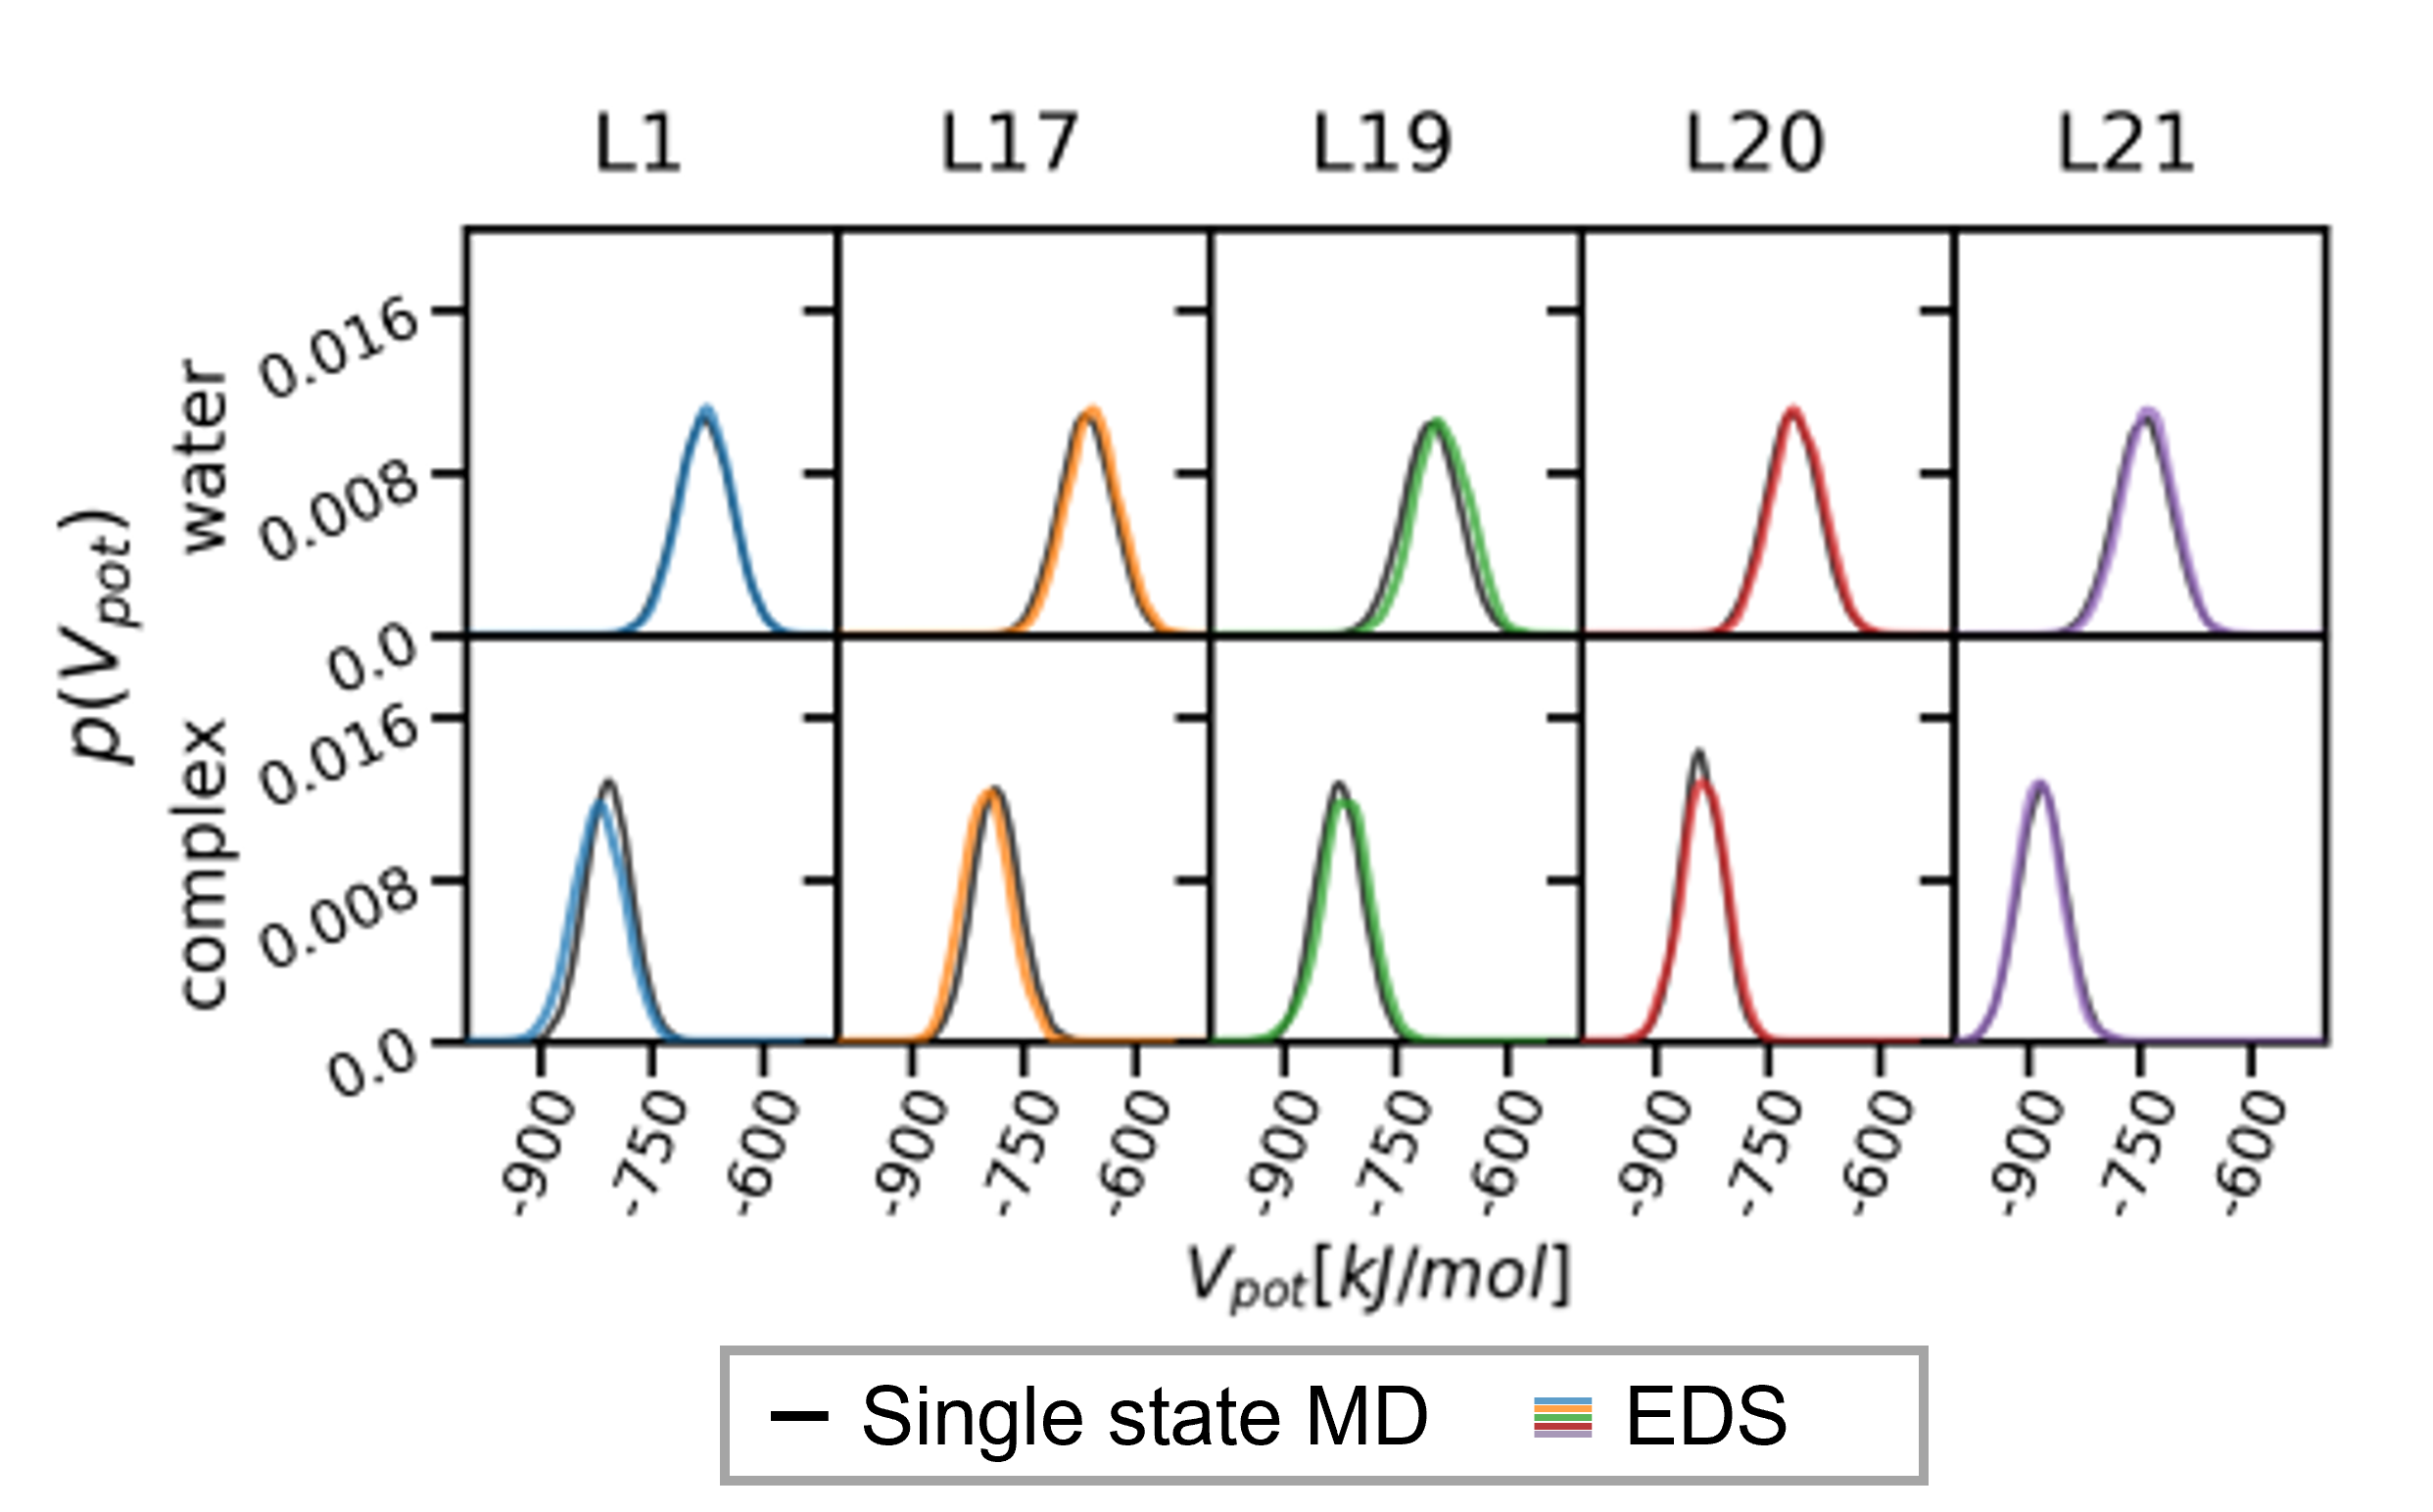
\includegraphics[width=0.8\textwidth]{fig/results/ringOpening/paramExploration/single_state_energy_sampling.png}
    \caption{Comparison of the potential-energy distribution obtained from a standard MD simulation of a given end state (black) and from an EDS simulation with the given end state favoured (colored) from the first step of the RE-EDS workflow.}
     \label{fig:CHK1_set2_stateOptimization_EnergyDistribution}
\end{figure}

\subsection{Energy Offset Estimation}
The relative energy offsets $\Delta \Delta E^R_{ji}$ are compared with the experimental relative binding free energies $\Delta \Delta G^\text{bind}_{ji}$ in Figure \ref{SIfig:Eoff_experiment_corr_RingOpening}. 
The RMSE between $\Delta \Delta E^R_{ji}$ obtained with RE-EDS 1SS and $\Delta \Delta G^\text{bind}_{ji}$ is $12.6$~kJ~mol$^{-1}$. Outliers are mainly related to L19.
With the RE-EDS SSM approach, the RMSE was reduced to $7.0$~kJ~mol$^{-1}$. No clear outliers were observed in this case. Thus, the use of the SSM approach is recommended for RE-EDS simulations.

%The energy offsets obtained with the SSM approach are shown as a function of the replica ($s$-value) in Figure \ref{SIfig:Eoff-perreplica}. 

\begin{figure}[H]
\centering
  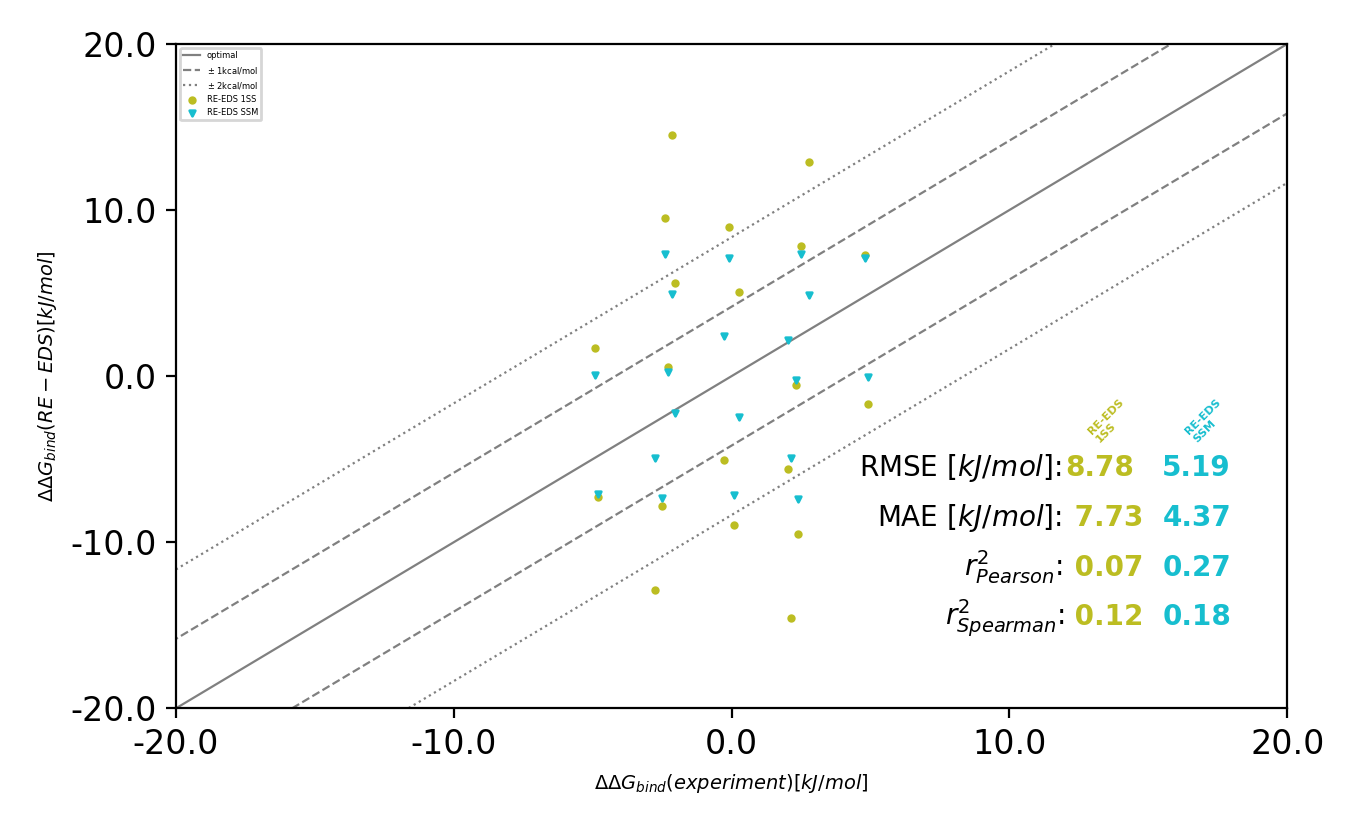
\includegraphics[width=0.8\textwidth]{fig/results/ringOpening/paramOptimization/RingClosure_system_Eoff_final_results.png}
\caption{Comparison of the relative energy offsets $\Delta \Delta E^R_{ji}$ in water and complex with the experimental relative binding free energies $\Delta \Delta G^\text{bind}_{ji}$. The energy offsets were estimated from RE-EDS simulations using the 1SS (green) or SSM (blue) approach to select the starting configurations of the replicas.} \label{SIfig:Eoff_experiment_corr_RingOpening}
\end{figure}


\subsection{Optimization of the $s$-Distribution and the energy offsets}
\begin{figure}[h]
\centering
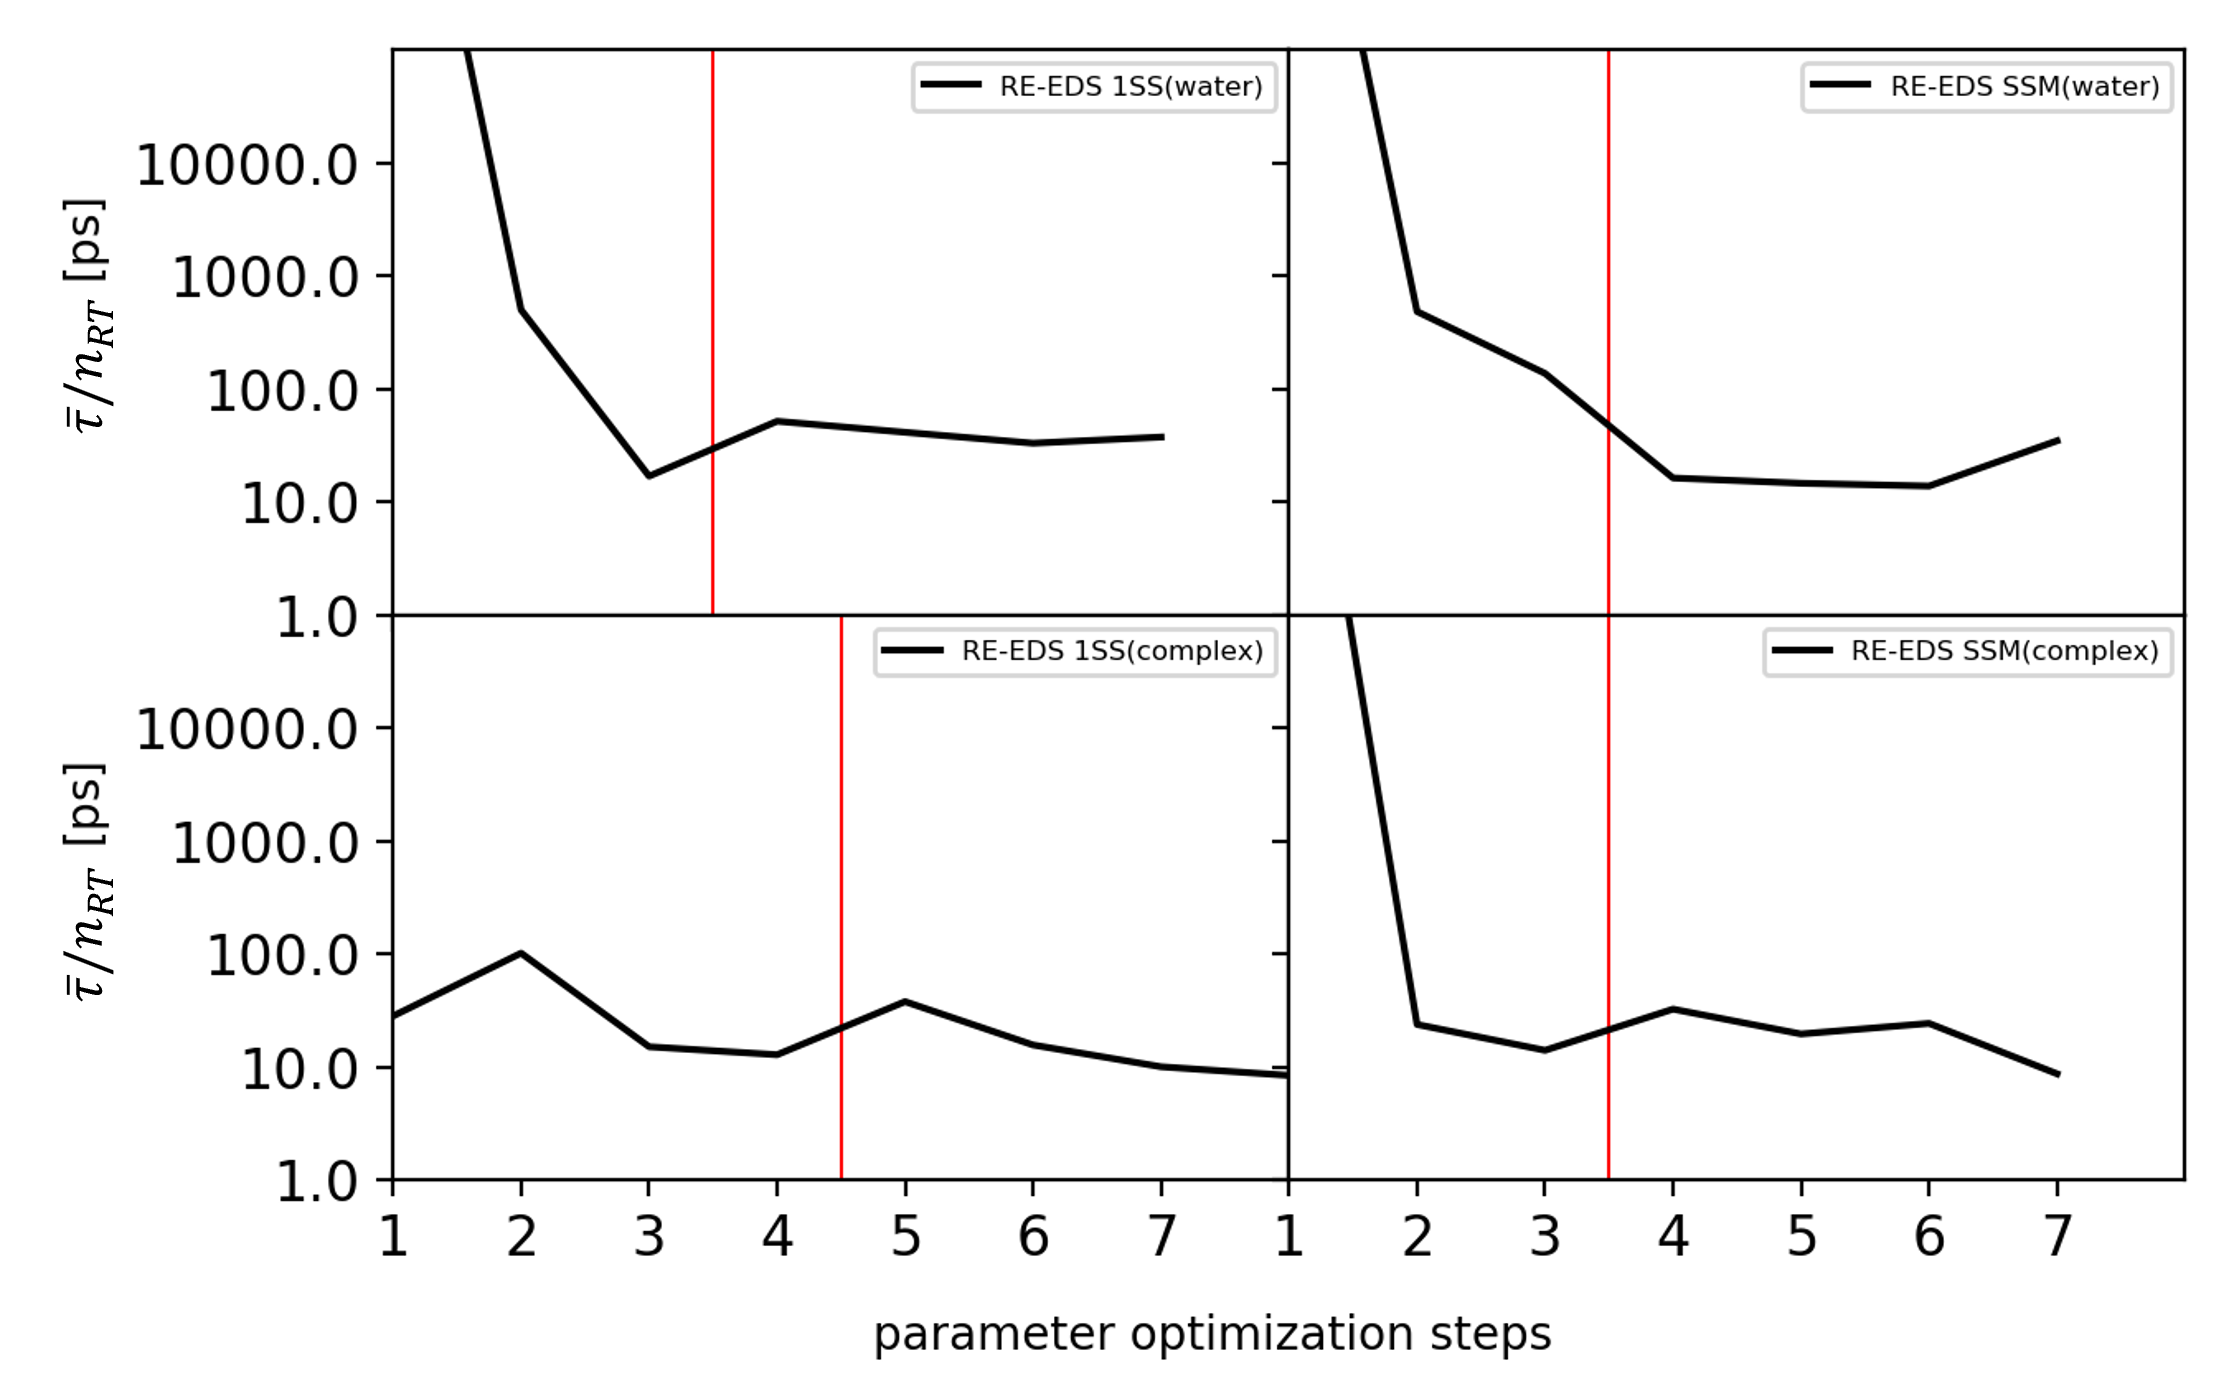
\includegraphics[width=\linewidth]{fig/results/ringOpening/paramOptimization/RingOpening_optimization_RTstat.png}
\caption{Average round-trip time as a function of the optimization steps $i$ ($\overline{\tau}_i$) on a logarithmic scale. The red line indicates the switch from $s$-optimization to energy offset rebalancing.}
\label{SIfig:CHK1_RingOpening_soptimization_efficiency}
\end{figure}

\begin{figure}[H]
\centering
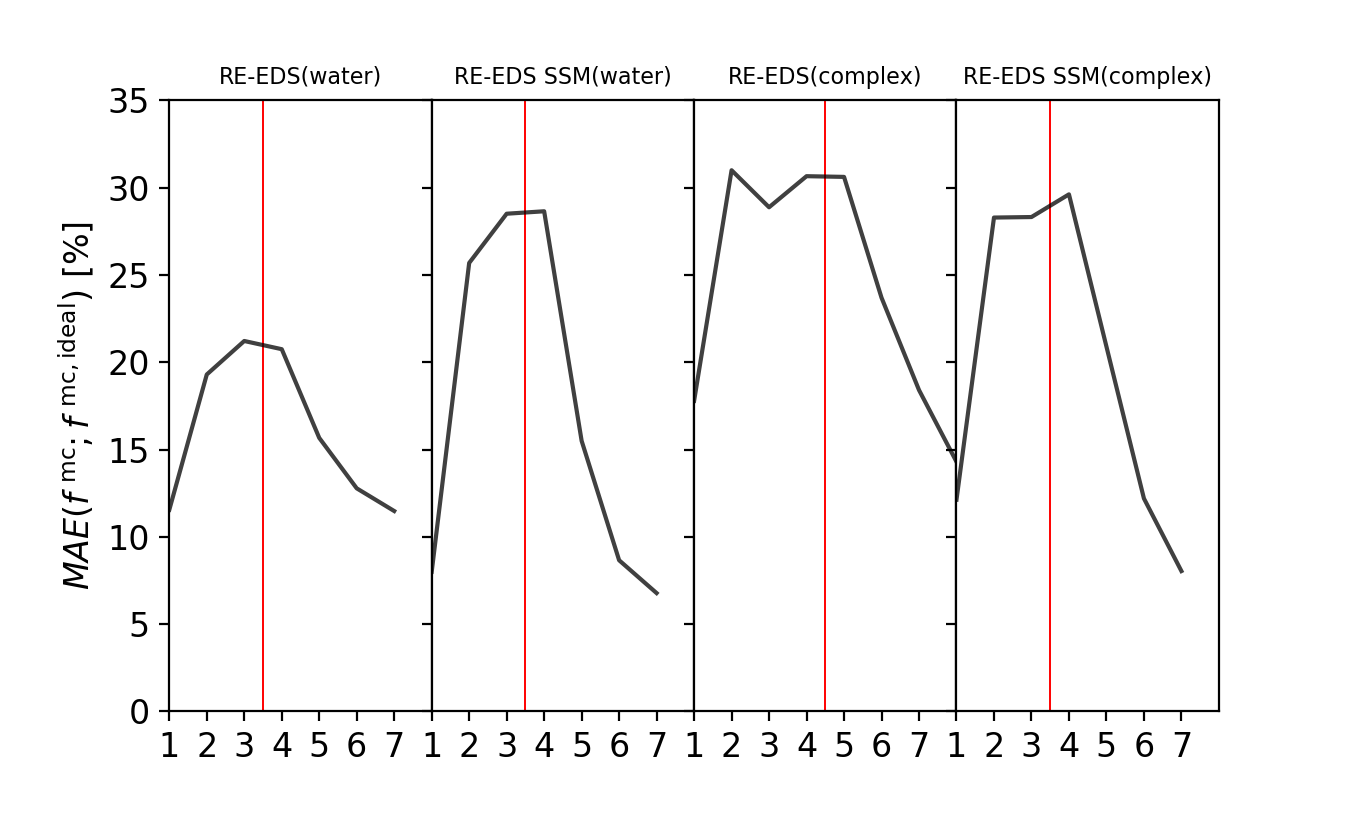
\includegraphics[width=\linewidth]{fig/results/ringOpening/paramOptimization/RingOpening_optimization_fractOptSampMAE.png}
\caption{Mean absolute deviation (MAE, in percentage) of the observed state sampling $f_i^{\text{mc}}$ from the ideal equal distribution $f_i^{\text{mc,ideal}}$ during the short optimization simulations. The red line indicates the switch from $s$-optimization to energy offset rebalancing.}
\label{SIfig:CHK1_RingOpening_optimization_fractOptSampMAE}
\end{figure}


\subsection{Free-Energy Calculation}
\begin{table}[H]
\caption{Free-energy differences in water and in complex calculated from the production run of 3.5~ns of length with the RE-EDS 1SS and RE-EDS SSM approaches.}
\begin{center}
\begin{tabular}{ c c |c c |c c}
  \multicolumn{2}{c|}{Ligand} & \multicolumn{2}{c|}{RE-EDS 1SS} &\multicolumn{2}{c}{RE-EDS SSM}\\ 
  J & I  & water [kJ~mol$^{-1}$] & complex [kJ~mol$^{-1}$]  & water [kJ~mol$^{-1}$] & complex [kJ~mol$^{-1}$] \\
  \hline
        L17 &         L1 &       11.9 $\pm$ 0.0&        17.0 $\pm$ 0.8&   12.4 $\pm$ 0.5&   9.4 $\pm$ 1.9\\
        L19 &         L1 &        2.7 $\pm$ 0.0&        5.7 $\pm$ 1.0&     3.1 $\pm$ 0.0&   8.0 $\pm$ 0.0\\
        L20 &         L1 &      -47.8 $\pm$ 0.0&      -47.6 $\pm$ 0.9& -47.7 $\pm$ 0.0&  -48.1 $\pm$ 0.0\\
        L21 &         L1 &      -61.7 $\pm$ 0.06&     -63.1 $\pm$ 0.8& -61.7 $\pm$ 0.0&  -64.8 $\pm$ 0.0\\
        L19 &         L17 &      -9.2 $\pm$ 0.0&      -11.3 $\pm$ 0.6&  -9.3 $\pm$ 0.5&   -1.4 $\pm$ 1.9\\
        L20 &         L17 &     -59.6 $\pm$ 0.0&      -64.5 $\pm$ 0.1& -60.1 $\pm$ 0.5&  -57.6 $\pm$ 1.9\\
        L21 &         L17 &     -73.6 $\pm$ 0.0&      -80.1 $\pm$ 0.1& -74.1 $\pm$ 0.5&  -74.3 $\pm$ 1.9\\
        L20 &         L19 &     -50.5 $\pm$ 0.0&      -53.2 $\pm$ 0.6& -50.7 $\pm$ 0.0&  -56.2 $\pm$ 0.0\\
        L21 &         L19 &     -64.4 $\pm$ 0.0&      -68.8 $\pm$ 0.6& -64.7 $\pm$ 0.0&  -72.9 $\pm$ 0.0\\
        L21 &         L20 &     -13.9 $\pm$ 0.0&      -15.5 $\pm$ 0.2& -14.0 $\pm$ 0.08& -16.7 $\pm$ 0.0 \\
\end{tabular}
\end{center}
\label{SItab: RE-EDS_FE_RingCycleOpening_dFs}
\end{table}

\begin{figure}[H]
\centering
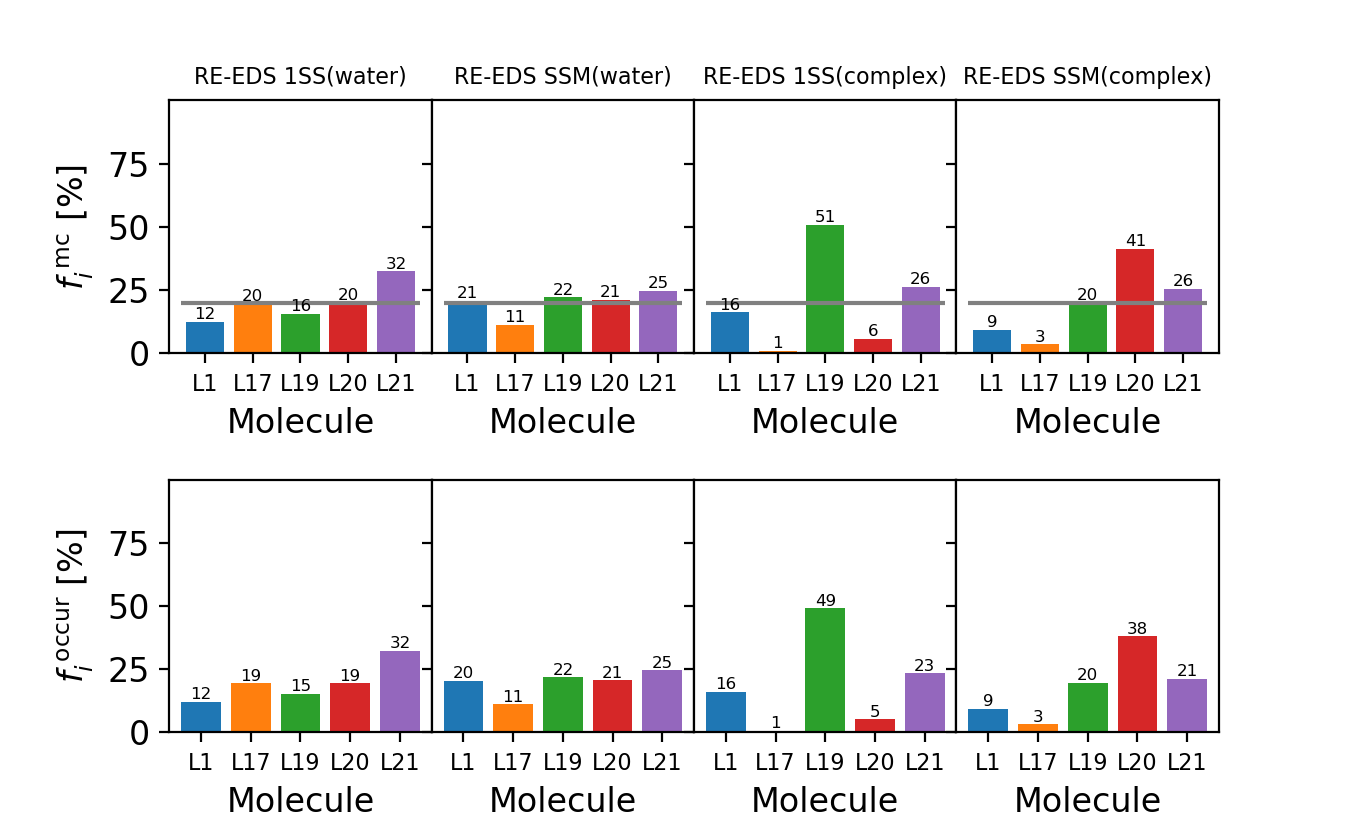
\includegraphics[width=\linewidth]{fig/results/ringOpening/FE/Reeds_RingOpening_production_sampling_s1.png}
\caption{Sampling of the end states in the final production run at replica $s=1.0$. Sampling was assessed by monitoring the maximally contributing end state (top panels) and by counting all end states a potential energy below $T_{i}^{phys}$ (see Table \ref{SItab:RingCycleOpenin_PotentialTresholds}) (bottom panels). Ideally, the sampling fraction as maximally contributing end state should be 1/$N$ (Eq. (8) in the main text) for all end states, indicated as a black horizontal line.}
\label{SIfig:CHK1_RingOpening_soptimization_final_Sampling_s1}
\end{figure}


\begin{figure}[H]
\centering
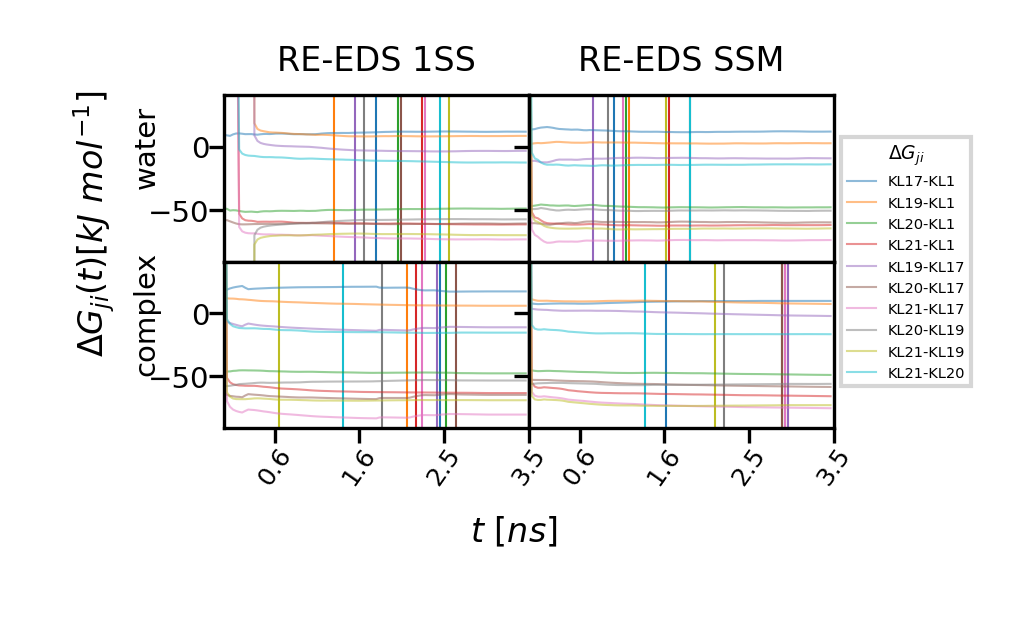
\includegraphics[width=\linewidth]{fig/results/ringOpening/FE/dF_RingOpening_Convergence.png}
\caption{Convergence analysis of the RE-EDS production runs (total 3.5~ns): The free-energy results are plotted as a function of the simulation time. The vertical lines indicate when a particular $\Delta G_{ji}$ value was found to be converged (deviation below 1~kJ~mol$^{-1}$).}
\label{SIfig:CHK1_RingOpening_dF_convergence}
\end{figure}


\clearpage
\newpage

%================================================================================
\section{Conclusion}
%================================================================================

This study reports the recent developments for the multistate free-energy method RE-EDS, which omits the definition of alchemical transition paths. The automatic workflow for RE-EDS was improved in robustness, and was applied to estimate the relative binding free energies of five CHK1 inhibitors containing typical core-hopping transformations. This system was investigated previously with FEP+ and QligFEP, allowing for a direct comparison of RE-EDS with state-of-the-art pairwise free-energy methods.
Using different starting configurations representing all end states (SSM approach) in the parameter optimization of the RE-EDS workflow improved the sampling, convergence, and the accuracy of the resulting free-energy differences. The performance of RE-EDS SSM was found to be comparable with FEP+ and QligFEP, and shows that RE-EDS with a ``dual topology" approach can be readily applied to challenging ligand transformations like ring size change, ring opening/closing, and ring extension.

In terms of computational efficiency, the total production run time with RE-EDS ($4$~ns per replica) was about half of that reported for FEP+ with this system. For RE-EDS, the simulation time could have been reduced further as the free-energy differences were found to be converged already after about $1$~ns. As multiple ligands are simulated simultaneously in a single RE-EDS simulation, this sampling enhancement will increase with increasing number of ligands. 
However, the pre-processing phase in the RE-EDS workflow currently uses a relatively large amount of simulation time. Making these steps more efficient will be addressed in future work.

The Python code for the RE-EDS workflow is provided on Github \\https://github.com/rinikerlab/reeds and can be used with the current version of GROMOS, freely available from http://www.gromos.net.

\clearpage
\pagebreak

%================================================================================
%\section{Appendix}
%================================================================================
\begin{ethappendix}
%================================================================================
%\appsection[CBTI and Quadrature]{quad}{Relationship between CBTI and Quadrature Integration}
%================================================================================

\end{ethappendix}
\clearpage
\pagebreak

%% %================================================================================
%% \begin{thebibliography}{74}
%% \input{\path/inc/paper.lrs}
%% \end{thebibliography}
%% %================================================================================

\end{document}
Classical molecular dynamics (MD) simulations provide insight into (bio-)molecular systems at atomic resolution, thereby explaining and complementing experimental observations. This often involves the calculation of free-energy differences\cite{CH10.1,CH11.8,HA14.1}, which characterize the relative stabilities of two or more macroscopic states of the system. These states may differ thermodynamically (different pressures, temperatures or numbers of molecules), conformationally (different regions in a space spanned by a set of specific generalized coordinates) or alchemically (different Hamiltonian functions). 

Alchemical free-energy calculations involve atom mutations or interaction alterations that have no experimental counterpart. However, by comparing the results of two such calculations in different environments (\eg{} mutation of a molecule into another one in vacuum or in a solvent) \textit{via} a thermodynamic cycle\cite{VA87.4,JO88.3}, the calculated values can be converted to experimentally accessible differences (\eg{} relative solvation free energies of the two molecules in the given solvent). This indirect pathway \textit{via} a cycle typically offers a strong sampling advantage relative to the calculation over a direct conformational path (\eg{} reversibly displacing the two molecules from vacuum into the solvent across the liquid surface), while giving the same result at full convergence\cite{CO14.1,MA17.14,BA18.2}. Over the last decades, numerous methods have been proposed to calculate alchemical free-energy differences between states $A$, $B$, $C$, ... of a molecular system involving the same numbers of atoms but different Hamiltonian functions. They can be roughly classified as reference-state methods and pathway-dependent methods\cite{SH07.13}.

In reference-state methods, a single simulation is performed at a reference state $R$ and the relative free energy of a target state $A$ is calculated using one-step free-energy perturbation\cite{ZW54.1,MA95.2,LI96.1,MA99.10,SC99.3,RA12.6,RA17.5,BO17.2} (OSP) as a free-energy estimator. The state $R$ may be unphysical, in which case the free-energy difference between two physical states $A$ and $B$ is obtained by comparing the results of two such calculations ($R$ to $A$ and $R$ to $B$). The accuracy of the method, \ie{} its convergence at finite sampling times, depends crucially on the extent of Boltzmann-weighted phase-space overlap between the reference and target
states\cite{LU01.1,LU01.2,HA10.3,BO17.2},
% NEW: HA10.3
%
\ie{} whether configurations relevant for $A$ are well sampled in $R$. Methods to enhance this overlap include in particular: 
($i$) the use of a reference state with soft-core\cite{BE94.1} (SC) sites\cite{MA95.2,OO03.1,OO04.2,KH11.2} 
or other softened force-field terms\cite{MA91.4,ME16.1,WA18.13,XI18.3};
% NEW: WA18.13 XI18.3
%
($ii$) the construction of a reference state encompassing all the target states, as in enveloping distribution sampling\cite{CH07.6,CH08.3,CH09.1,CH09.3} (EDS);
($iii$) the extension to the use of multiple reference states\cite{KH11.2}, along with the application of 
the (multi-state\cite{SH08.7}) Bennet acceptance ratio\cite{BE76.3,SH03.5} (BAR or MBAR) estimator instead of OSP.
In principle, reference-state methods bear the promise of enabling the extrapolative calculation of the relative free energies of numerous arbitrary states ($A$, $B$, $C$, ...) based on a single reference-state simulation. In practice, however, they seldom hold this promise (or not in a sufficiently robust fashion based on finite simulations), because the design of a suitable reference state requires considerable (\eg{} SC approach) or even complete (\eg{} EDS approach) \textit{a priori} knowledge of the target states it has to be appropriate for.

In pathway-dependent methods, a hybrid Hamiltonian is constructed by employing a coupling parameter $\lam$ that defines a continuous transformation between the Hamiltonians of the physical end-states $A$ and $B$. Given such a path, the most established, robust and still frequently used method 
is \revphil{multi-configuration\cite{ST91.1}} thermodynamic integration\cite{KI33.1,KI34.2,KI35.1} 
%(TI). 
\revphil{(MCTI or, simply, TI)}.
In TI, a set of 
independent simulations are performed at different constant $\lam$-values, and the 
ensemble average of the derivative of the hybrid Hamiltonian with respect to $\lam$ is 
subsequently integrated by numerical quadrature\cite{JO10.2,BR11.5,BR11.6} 
%
or curve fitting\cite{SH09.12,JO10.2,VI10.6,SH11.7}.
%
\revphil{A common alternative to TI is multi-configuration\cite{JO08.3}
free-energy perturbation\cite{ZW54.1,MA95.2,LI96.1,MA99.10,SC99.3,RA12.6,RA17.5,BO17.2} (MC-FEP or, simply, FEP),
where the OSP estimator is used to evaluate the free-energy difference
from one $\lambda$-point to the previous or/and next one.}
%
Refinements and improvements of \revphil{the original TI protocol} include in particular:
($i$) the design of Hamiltonian coupling schemes 
%with 
leading to high sampling efficiencies;\cite{CR86.1,BL04.2,PH11.1,PH12.1,NA14.1,NA15.3}
($ii$) the partial automation of the TI protocol\cite{ME93.3,HU16.7,ME17.1,SU17.3,DA18.1}, 
\ie{} of the selection of $\lam$-points along with associated \revphil{initial configurations,} equilibration \revphil{times} and sampling times;
($iii$) the use of free-energy estimators with improved statistical efficiencies over plain quadrature, \eg{} extended TI (EXTI) estimator\cite{DE16.9} or MBAR estimator\cite{SH08.7};
($iv$) the design of alternative single- or multiple-replica schemes where the $\lam$-values are
no longer fixed during the simulation\cite{LI93.1,TI93.2,KO96.1,SU99.1,MI01.1,IB01.1}. 

Although the possibility of changing the $\lam$-values over the course of a simulation may appear at first sight to represent an unnecessary complication of the TI protocol, it often leads to a significant enhancement of the sampling efficiency. This is because it increases the likelihood of crossing barriers 
\revphil{in the orthogonal space\cite{BI15.1,GR16.4},
%
%\ie{} the space spanned by all conformational degrees of freedom excluding $\lam$. 
that is, the space spanned by all the 
%conformational 
degrees of freedom of the system excluding $\lam$ ({\em i.e.} all the conformational ones). 
}
%
These orthogonal barriers are typically higher at certain $\lambda$-values than at others. 
The highest ones may be seldom crossed in corresponding simulations at \radd{fixed $\lam$, and}
allowing for variations of $\lam$ may open pathways to circumvent them. Note that, in many cases, this enhancement is not sufficient \textit{per se} and other techniques must be applied to further 
improve the orthogonal sampling 
%
%along the $\lam$-path\cite{WO03.1,WO03.2,HR07.1,DE08.2,DE08.12,FA08.7,HR08.1,HR09.1,GA13.4,KH10.1,KH11.2,DO12.5,WA12.2,GA13.4,KA14.3,ME16.1}. 
along the $\lam$-path\cite{WO03.1,WO03.2,HR07.1,DE08.2,DE08.12,FA08.7,HR08.1,HR09.1,KH10.1,KH11.2,DO12.5,WA12.2,GA13.4,KA14.3,ME16.1}. 
%
There exist two main routes for performing variable-$\lam$ simulations:
($i$) Hamiltonian replica exchange (HRE) or permutation (HRP), which involve multiple system replicas;
($ii$) $\lam$-dynamics ($\lam$D) or $\lam$-Monte Carlo ($\lam$MC), which consider a single system.

In the HRE scheme\cite{SU99.1,FU02.2,ZH16.2}, a series of system \revphil{copies (walkers)}
are distributed over a set of fixed $\lam$-values \revphil{(replicas)}, 
as is the case in TI. However, at regular time intervals, swaps are attempted 
between pairs of systems corresponding to different $\lam$-values (typically adjacent ones).
%$\lam$-values). 
These attempts are accepted or rejected according to a Metropolis-Hastings criterion\cite{ME53.1,HA70.4} depending on the Boltzmann factor ratio of the replica system before and after the swap. Although the trajectories at each $\lam$-point become discontinuous, the TI-like statistics is preserved and the data can be analyzed in the same way as for TI. Recent extensions of the method involve in particular the consideration 
of 
%
more advanced exchange schemes\cite{CA05.6,BR07.6,CH11.9}, 
%
%
of replica reservoirs\cite{LI06.11,OK07.4,RO07.14,RU10.2,OK13.1,HE13.6,DA18.6},
%%% NEW OK07.4 RU10.2 HE13.6 DA18.6
%
of frozen replicas\cite{CH15.28,CH16.21},
%
\radd{of heating-quenching steps between the sampling periods\cite{LI07.13,LI09.20,LI15.18,HE13.6,KU18.3},}
%
%(TIGER)
% NEW: ALL
%
%Temperature Intervals with Global Energy Reassignments (TIGER)
%  Original ref for TIGER
%    **  LI07.13 : [Li/Stuart] An improved replica-exchange sampling method: Temperature intervals with
%              global energy reassignment.
%  Original ref for TIGER2
%    *** LI09.20 : [Li/Stuart] TIGER2: An improved algorithm for temperature intervals with global exchange
%              of replicas.
%  Original ref for TIGER2A
%    **  LI15.18 : [Li/Latour] TIGER2 with solvent energy averaging (TIGER2A): An accelerated sampling
%              method for large molecular systems with explicit representation of solvent.
%  Original ref for TIGER2h
%    KU18.3  : [Kulke/Langel] Replica-based protein structure sampling methods: Compromising between
%              explicit and implicit solvents.
%  Implementations
%    ME10.6  : [Menz/Biggs] TNAMD: Implementation of TIGER2 in NAMD.
%    BR15.12 : [Brown/Walsh] An improved TIGER2 implementation for NAMD suitable for the Blue Gene
%              architecture.
%  Applications
%    * HE13.6  : [Henriksen/CheathamIII] Reliable oligonucleotide conformational ensemble generation 
%                in explicit solvent for force field assessment using reservoir replica exchange molecular 
%                dynamics simulations. 
%
%
of the infinite-swapping limit\cite{SI08.3,PL11.4,DU12.3,PL13.3,LU13.4,ZH16.2},
% (ISL),
%
\radd{and of generalized-ensemble distributions\cite{KI10.5,LU12.7,LU13.5,LU14.6,MA15.18,MA15.19}}.
% (gREM)}.
% NEW: ALL
%KI10.5  : [Kim/Straub] Generalized replica exchange method. 
%LU12.7  : [Lu/Straub] Exploring the solid-liquid phase change of an adapted Dzugutov model using 
%          generalized replica exchange method. 
%LU13.5  : [Lu/Straub] Order parameter free enhanced sampling of the vapor-liquid transition using 
%          the generalized replica exchange method. 
%LU14.6  : [Lu/Straub] Investigating the solid-liquid phase transition of water nanofilms using the 
%          generalized replica exchange method. 
%MA15.18 : [Ma\l{l}olepsza/Keyes] Isobaric molecular dynamics version of the generalized replica
%          exchange method (gREM): Liquid-vapor equilibrium.
%MA15.19 : [Ma\l{l}olepsza/Keyes] Water freezing and ice melting.
%
%
%
They also include the implementation of $\lam$-moves that go beyond pairwise swaps with a selection based on a Suwa-Todo criterion\cite{SU10.4,TO13.7,MO15.11}, as implemented in the HRP method\cite{IT13.1,IT13.2,YA17.2}. In the latter case, enabling arbitrary permutations and abandoning the detailed-balance constraint leads to a \radd{significant} increase in the probability of exchange acceptance.


In the $\lam$D scheme \cite{KO96.1,DA01.7,GU03.1,KN09.1,KN11.2,DO11.2,AR15.2,HA17.1} (see also its ancestor\cite{TI93.2,LI93.1} $\lam$MC), a single system is considered for which the $\lam$-value evolves dynamically in the course of the simulation, \ie{} $\lam$ is treated as an extra pseudo-conformational degree of freedom with an assigned mass parameter $m_{\lam}$ and momentum $p_{\lam}$. This momentum enters an extended Hamiltonian that includes an additional term for the corresponding kinetic energy. This results in a continuous sampling of the $\lam$-range instead of the discrete sampling underlying TI or HRE/HRP. The free-energy difference is then typically estimated from the probability distribution along $\lam$, with the drawback of requiring a threshold to define the end-states\cite{KN11.1}. This issue can be alleviated by introducing a coordinate transformation with plateaus\cite{BI14.1,BI15.2}, or by using a TI-like formula\cite{KA05.1,KA06.6,KA12.5} or a Rao-Blackwell estimator\cite{DI17.5}, the latter conceptually similar to MBAR. 

The major advantages of $\lam$D compared to HRE/HRP are that it involves a simpler single-system setup, is deterministic, 
samples the $\lam$-range continuously, and does not require the specification (and 
optimization\cite{KO05.8,RA05.8,TR06.5,SI08.3,NA08.6,NA08.10,VO15.2,VO15.3,ZH16.2,SI16.5,SU17.3,SI17.7,MA18.8})
%%% NEW AB08.3 SI17.7
%
of a $\lam$-ladder and of a swapping-attempt frequency. The main drawback\cite{BI14.1} is that 
the sampling probability along $\lam$ is no longer imposed in the form of a fixed set of $\lam$-points 
with equal sampling times, but entirely controlled by the free-energy profile along $\lam$. 
As a result, $\lam$-values with high relative free energies may be poorly represented (or not at all) 
and $\lam$-barriers with high relative free energies may be seldom crossed (or not at all) in the 
course of a finite simulation. In addition, care must be taken to avoid the sampling of $\lam$-values 
beyond the physical end-states of the alchemical coupling\cite{KO96.1} \revphil{({\em i.e.} below 0 or above 1)}. 
%
Both the sampling inhomogeneity and the end-point issues can in principle be remedied\cite{BI14.1} 
by employing an appropriate coordinate transformation\cite{KN11.2,DO11.2,WU11.1,KN11.1,DO13.1,ZH12.3,BI14.1,BI15.2} or/and 
by applying a biasing potential along $\lam$\cite{GU98.1,GU98.2,SO01.1,WU11.1,BI14.1,BI15.2}. A combination of these two 
approaches underlies the $\lambda$-local elevation umbrella sampling method\cite{BI14.1,BI14.2,BI15.1,BI15.2} ($\lam$-LEUS), 
which relies in particular on an adaptive memory-based biasing potential. 
%
%Note that 
A similar principle is also at the heart of numerous other methods such 
as the flat-histogram\cite{WA01.5,LA04.6}, $\lam$-metadynamics\cite{LA02.1,BA08.2,WU11.1}, 
adaptive integration\cite{FA04.3}, adaptive biasing force\cite{DA08.2}, \radd{adaptively biased\cite{BA08.1}} 
and expanded-ensemble\cite{LY92.1,LY94.1,LY96.2,ES07.1,ES07.2,PA11.7,RA18.2} methods. 

In $\lam$-LEUS, a local elevation\cite{HU94.3} (LE) build-up phase is used to construct a suitable biasing potential, and followed by an umbrella sampling\cite{TO74.1,TO77.1} (US) phase where this potential is frozen\cite{HA10.1} and biased equilibrium statistics gathered with quasi-homogeneous sampling of the $\lam$-range. Clearly, the LE phase represents an efficiency loss in the method, \ie{} a dead time. Note, however, that a similar (but generally shorter) dead time also exists in TI and HRE/HRP in the form of discarded initial equilibration times for all replicas. Another drawback of $\lam$-LEUS is that it is not parallelizable in the same fashion as TI and HRE/HRP, where the simulations at different $\lambda$-points can be carried out in parallel (see, however, various swarm\cite{HU98.6,BU15.5,KA18.6,AL18.2}, multiple-walker\cite{RA06.2,CO14.5} and flying Gaussian\cite{SU16.3,KR17.1} variants of memory-based biasing methods). 
Finally, some care must be taken to select \radd{an appropriate mass and thermostat-coupling scheme 
for the $\lam$-variable, so as to ensure that 
this variable is adequately coupled to the configurational degrees of freedom\cite{BI15.1}.}
%can have a significant influence on the calculation results

In the present chapter, we propose a new alchemical free-energy calculation scheme with the goal of combining the advantages and alleviating the shortcomings of both HRE/HRP and $\lam$D. This scheme is termed conveyor belt thermodynamic integration (CBTI) and relies on the coupled $\lam$D of a set of system replicas, in which the $\lam$-distance between successive replicas is kept fixed along a forward-turn-backward-turn path, akin to a conveyor belt between the two physical end-states. The basic principle of CBTI is illustrated schematically in \reffig{scheme}.

Considering a free-energy profile $G(\lam)$ presenting a constant uphill slope between $A$ and $B$, a single system subjected to $\lam$D in the absence of a biasing potential will ``roll down'' to $A$ and keep sampling the neighborhood of this state (\reffig{scheme:ldyn:plane}). To circumvent this problem, one may decide to couple the $\lam$D of two replicas 0 and 1 of the system in such a way that any downhill displacement of replica 0 implies an equivalent uphill displacement of replica 1 (\reffig{scheme:cvb:plane}). This working principle is exploited in practice by vehicles like cable cars or funiculars, where the motion of the two vehicles are controlled by a stretched cable connected to two pulleys. It has also been exploited previously for MD in the context of twin-system\cite{HA13.1,GE16.1} EDS, which couples forward and reverse alchemical changes performed in two different environments. In this situation, one may describe the $\lam$-values of the two replicas by means of a single periodic angular variable $\Lamb$ representing the advance of the cable from 0 (replica 0 in state $A$, replica 1 in state $B$) to $\pi$ (0 in $B$, 1 in $A$) and then $2\pi$ (back to the starting situation). Note that the $\pi$ to $2\pi$ return range of $\Lamb$ deviates from the cable car or funicular analogy, where the vehicles never go ``over the pulley''. If the free-energy profile $G(\lam)$ has a constant slope, it is easily seen that there will be no net driving force on the cable. In the $\lam$D context, this means that the $\Lamb$-variable will undergo random diffusion with a homogeneous sampling of $\Lamb$, \ie{} the corresponding free-energy profile $G_{\Lamb}(\Lamb)$ will be flat (\reffig{scheme:ene:plane}). Accordingly, each of the two replicas will sample the entire $\lam$-range homogeneously.

\begin{figure}[!ht]
  \centering
  \subgraph{fig:scheme:ldyn:plane}{lambda_dyn_linear.pgf}{.49}%
  \hfill%
  \subgraph{fig:scheme:ldyn:gotoflat}{deltag_example_ene_ana.pgf}{.49}%

  \vspace{-1em}
  \subgraph{fig:scheme:cvb:plane}{conveyor_belt_linear.pgf}{.49}%
  \hfill%
  \subgraph{fig:scheme:ene:plane}{ene_0.pgf}{.49}
  
  \vspace{-1em}
  \subgraph{fig:scheme:cvb:zigzag}{conveyor_belt_zigzag.pgf}{.49}%
  \hfill%
  \subgraph{fig:scheme:ene:zigzag}{ene_1.pgf}{.49}

  \vspace{-1em}
  \subgraph{fig:scheme:cvb:sinus}{conveyor_belt_sintw.pgf}{.49}%
  \hfill%
  \subgraph{fig:scheme:ene:sinus}{ene_2.pgf}{.49}\\
  
  \caption{\footnotesize
\textit{Schematic illustration of the conveyor belt thermodynamic integration (CBTI) approach for different free-energy profiles $G(\lam)$ and numbers of replicas $K$.} The free-energy profile $G(\lam)$ is shown on the left along with the conveyor belt for an inclined plane (\subref{fig:scheme:cvb:plane}), a piecewise-linear curve (\subref{fig:scheme:cvb:zigzag}) and a more realistic curve (\subref{fig:scheme:cvb:sinus}),
\radd{the latter curve corresponding to the function}
%illustrative function of Panel (\subref{fig:scheme:cvb:sinus}) 
%is 
$G(\lam)=\sin (\pi \lam)(\lam-0.5)^2+0.25\lam$.
%
The corresponding free-energy profiles $G_{\Lamb}(\Lamb)$ 
along the conveyor belt advance variable $\Lamb$ \revphil{(\refeq{fre_prof_lam_def})} are shown on the right for $K=2$ (blue), $K=4$ (red), $K=8$ (green) or $K=16$ (orange).
%
The top-left panel (\subref{fig:scheme:ldyn:plane}) illustrates the situation of plain unbiased $\lam$D, 
where the system would ``roll down'' the slope and keep sampling the neighborhood of the state with the lowest free energy.
%
\radd{The top-right panel (\subref{fig:scheme:ldyn:gotoflat}) 
shows the height $G^\star_{\Lamb}$ of the residual barriers in the 
free-energy profile $G_{\Lamb}(\Lamb)$ considering this illustrative function
and increasing values of $K$.
The data is represented in logarithmic form and a linear line of slope $-1$ is fitted to the filled 
      circles.
}
}
  \label{fig:scheme}
\end{figure}

Consider now a free-energy profile $G(\lam)$ presenting a constant uphill slope from 0 to $1/2$ and a constant downhill slope from $1/2$ to 1 (\reffig{scheme:cvb:zigzag}). In a setup with two replicas, the $G_{\Lamb}(\Lamb)$ profile will no longer be flat (\reffig{scheme:ene:zigzag}, blue curve). From 0 to $\pi/2$ and from $\pi$ to $3\pi/2$, both replicas move uphill, whereas from $\pi/2$ to $\pi$ and from $3\pi/2$ to $2\pi$, they both move downhill. This can be remedied by using four instead of only two replicas, placed at equal distances along the cable. This working principle is now more reminiscent of the real-life situation of a conveyor belt. In this four-replica setup, the $G_{\Lamb}(\Lamb)$ profile will again be flat (\reffig{scheme:ene:zigzag}, red curve), and each of the four replicas will sample the entire $\lam$-range homogeneously.

Finally, consider a more realistic free-energy profile $G(\lam)$ (\reffig{scheme:cvb:sinus}). 
In the general case, the $G_{\Lamb}(\Lamb)$ profile will never be exactly flat irrespective 
of the number $K$ of replicas. However, by adding more and more replicas to the conveyor belt, 
the features of the $G_{\Lamb}(\Lamb)$ profile can be progressively reduced in magnitude 
(as illustrated for $K=2$, 4, 8 or 16 replicas by the blue, red, green and orange curves of \reffig{scheme:ene:sinus}). 
%
%
Note that \revphil{we restrict} the choice of $K$ to even values, 
in order to have always the same number of replicas moving forward and backward. 
% The choice of an odd number of replicas would break the forward-backward symmetry, with one extra replica moving in either of the two directions.
\revphil{Although the choice of an odd number of replicas would be acceptable, 
it is likely to be less favorable (especially at small $K$), because 
one extra replica would always move in either of the two directions.
}

\revphil{Considering the illustrative $G(\lambda)$ of \reffig{scheme:cvb:sinus}, 
the magnitude $G^{\star}_{\Lambda}$ of the variations 
in $G_{\Lambda}(\Lambda)$ is shown in \reffig{scheme:ldyn:gotoflat} as a function of $K$.}
%
As discussed in \refsec{quad}, 
these variations
%in the $G_{\Lamb}(\Lamb)$ profile 
can be interpreted as
the residual of a $K$-point trapezoid quadrature approximation to the vanishing integral of the derivative of an even periodic function \radd{over one period, namely that of the $G(\lam)$ profile after mirroring}. Quantitatively, this interpretation shows that the magnitude $G^{\star}_{\Lambda}$ of 
these variations decreases at least as $K^{-1}$ \radd{in the limit of large $K$}. 
%
%
Note that the convergence to a flat 
%$G_{\Lamb}(\Lamb)$ 
\revphil{profile
({\em i.e.} the decrease
of the barrier heights towards zero upon increasing $K$)}
does not need to be regular for small $K$ (see \eg{} the comparatively low variations for the blue curve in \reffig{scheme:ene:sinus}) and that it can be stronger than $K^{-1}$ \radd{for large $K$} if $G(\lam)$ presents particular continuity/symmetry properties.
%
By \radd{using a sufficient number of replicas}, one may thus ensure a quasi-homogeneous sampling of the $\lam$-range by each replica, even in the absence of coordinate transformation or biasing potential. If desired, a memory-based biasing potential may still be applied to further homogenize the sampling. However, the LE build-up time 
%will 
can
be considerably reduced relative to that needed in a corresponding single-system $\lam$-LEUS simulation, \radd{because this biasing potential} only needs to be applied to the $\Lamb$-variable and no longer to the $\lam$-variable. Thus, it has to compensate for comparatively small $G_{\Lamb}(\Lamb)$ variations. Furthermore, it only needs to be constructed over a limited $\Lamb$-range, considering that $G_{\Lamb}(\Lamb)$ is periodic with period $2\pi K^{-1}$ as well as even over this $2\pi K^{-1}$ interval. 

Irrespective whether a biasing potential is employed or not, the definition of a free-energy estimator for the CBTI scheme, \ie{} a procedure to construct $G(\lam)$ based on the simulation results for the multiple-replica system, is not as trivial\cite{KR17.1} as in the single-system $\lam$D or $\lam$-LEUS cases. Here, CBTI is analyzed using a TI-like estimator\cite{KA05.1} relying on the quadrature integration of the \radd{average} Hamiltonian $\lam$-derivative binned \radd{along $\lambda$} considering all replicas \radd{simultaneously}. The associated quadrature error can be kept very low by using a large number of bins, which is rendered possible by the continuous and quasi-homogeneous $\lam$-sampling. 
%
Although this estimator is very robust, we note that it may not be optimal in terms of statistical efficiency\cite{LU04.3,SH05.6,SH08.7,FA09.4,TA12.1,DE16.9,DI17.5,ZH17.6}. 


In the present chapter, we provide the mathematical/physical formulation of the proposed CBTI scheme, and report an initial application of the method to an illustrative alchemical transformation: the mutation of a methanol molecule to a dummy (non-interacting) skeleton in water, giving access to the hydration free energy of the molecule.
%------------------------------------------------------------
\subsection{Test System}
%------------------------------------------------------------

As an initial application of the proposed CBTI scheme, we considered here 
a relatively simple perturbation, namely the conversion of methanol
from a fully interacting molecule to a dummy skeleton (no intermolecular interactions) 
in an aqueous environment at $P=1\unit{bar}$ and $T=298.15\unit{K}$.
%
The calculations were performed using 
\radd{a modified version of the 
GROMOS11 program \cite{VA11.7,SC12.1,KU12.1} along with}
the parameters of the GROMOS-compatible 2016H66 force field\cite{HO16.1} for methanol\cite{HO11.1} (united-atom, rigid bonds, flexible bond-angle)
and the simple point charge (SPC) model\cite{BE81.1} for water (fully rigid).
%
Since the dummy skeleton retains the intramolecular interactions (here, only the bond-angle),
the calculated free-energy change $\Delta G$ corresponds directly to minus the hydration 
free energy of methanol.


Possible issues related to the existence of a singularity\cite{SI93.1,BE94.1,ZA94.1} 
and the insufficient solute-solvent kinetic-energy exchange\cite{SH03.4,SH05.7,MO07.2,LI08.8} 
close to $\lambda=1$ were alleviated in the usual way,
by means of a soft-core scheme\cite{BE94.1} for the alchemical coupling 
and of stochastic dynamics\cite{LA08.6,VA88.1} (SD) for thermostating the solute and solvent conformational 
degrees of freedom.
%
In most CBTI simulations, the \radd{instantaneous} temperature $T_\Lambda$ of the CB advance variable
$\Lambda$ was also controlled separately by means of a 
Nos\'e-Hoover chain thermostat\cite{MA92.1} 
\radd{at 298.15 K} \revphil{(eight successive thermostat variables)},
with a coupling time $\tau_{\Lamb}$.

%------------------------------------------------------------
\subsection{Simulations Sets}
%------------------------------------------------------------

The exploration of the CBTI scheme and the comparison of its
performance with that of existing methods was carried out in five successive 
steps:
%
($1$) establishing reference TI results;
($2$) analyzing the influence of the CBTI parameters (number $K$ of replicas along with the
       mass-parameter $m_\Lambda$ and thermostat coupling time $\tau_\Lambda$ 
       of the CB advance variable);
($3$) investigating the use of a biasing potential;
($4$) examining the features of the TI-like free-energy estimator (effect of the number $J$ of integration bins and use of equations without specification of $J$);
($5$) comparing the results of CBTI with those of existing methods.


The reference TI calculations (Step 1) were performed using $K_{\mathrm{TI}}=2^n+1$ 
equidistant $\lambda$-points covering the range $[0,1]$  with $n$ = 1,2,...,7.
They involved initial configurations equilibrated for $0.2\,\mathrm{ns}$ 
starting from the equilibrated configuration at the previous $\lam$-point,
\radd{and a simulation time of $100 K_{\mathrm{TI}}^{-1}$ ns per $\lambda$-point.}
%
Each of these calculations, \radd{involving a total single-system sampling time of 100 ns},
was repeated ten times using different random initial velocities. 
%
The integration over the average Hamiltonian derivative 
was 
%then 
performed based on \refeq{ti_formula} using the Simpson quadrature rule\cite{JO10.2,BR11.5,BR11.6}.


To explore the influence of the CBTI parameters (Step 2), various 
combinations of $K$, $m_\Lambda$ and $\tau_\Lambda$ were considered in 
three series of calculations, namely:
%
($i$) the choices $m_{\Lambda}={16,160,800,1600~\text{or}~3200}\,\mathrm{u}\,\mathrm{nm}^2$
       (where $\mathrm{u}$ stands for atomic mass unit, {\em i.e.} g mol$^{-1}$),
      along with $K=16$ replicas in the absence of thermostat coupling 
      for $\Lambda$, {\em i.e.} with $\tau_\Lambda\rightarrow\infty$;
%%      ($10\unit{ns}$ simulations of the replica system after $0.2\unit{ns}$ equilibration);
%
($ii$) the choices $\tau_\Lambda={0.05,0.1,0.5,1~\text{or}~2}\,\mathrm{ps}$
       along with $K=16$ replicas and $m_{\Lambda}=160\,\mathrm{u}\,\mathrm{nm}^2$;
%%      ($10\unit{ns}$ simulations of the replica system after $0.2\unit{ns}$ equilibration);
%
($iii$) the choices $K=8,16,32,64~\text{or}~128$
       along with 
       $m_{\Lamb}=40 K^{1/2}\,\mathrm{u}\,\mathrm{nm}^2$ 
       and $\tau_{\Lambda}=0.5\,\mathrm{ps}$;
%% ($256 K^{-1}\unit{ns}$ simulations of the replica system after $0.2\unit{ns}$ equilibration).
%
%
The parameters (and results) of these three series of simulations, including their durations $t_{\mathrm{sim}}$, are summarized  in \reftab{screen} (entries 1-15).
%
\radd{All these simulations were preceded by $0.2\unit{ns}$ equilibration}.
%
\revphil{
For the the third series (entries 11-15), $m_{\Lambda}$ was made proportional 
to $K^{1/2}$, an arbitrary parameter choice justified by arguments provided 
in \refsec{othersim}, and the five simulations relied on the 
the same total single-system sampling time of 256 ns.}
%
%
This exploration showed that the CBTI method is rather robust with respect to the choice of its parameters.
The values $K=16$, $m_\Lamb=160\,\mathrm{u}\,\mathrm{nm}^2$ and $\tau_{\Lamb}=0.5\,\mathrm{ps}$ 
were retained as 
%an optimal combination
\revphil{a good combination}
for the alchemical perturbation considered.
\radd{For comparison with the TI results of Step 1,}
ten repeats of the calculation 
involving this specific choice were performed using different random initial velocities
and 
\radd{a total single-system sampling time of 100 ns after $0.2\unit{ns}$ equilibration}.
%
%($6.25\unit{ns}$ simulations of the replica system after $0.2\unit{ns}$ equilibration, \ie{}  total $100\unit{ns}$ single-system sampling time).
%



\begin{table}[H]
\caption{
  \textit{Influence of the CBTI parameters in 
%\revdavid{[DELETE: unbiased]}
 simulations 
  of the aqueous methanol-to-dummy mutation at 298.15 K and 1 bar with the 
  2016H66 force field.}
%
  \revphil{This table investigates the influence of the parameters selected for the CBTI scheme
           on the temperature and dynamics of the CB advance 
           variable $\Lambda$ and on the calculated free-energy change $\Delta G$
           (for the latter, considering a constant total single-system sampling time of 100 ns).
           }
%
  \radd{For each simulation,} the successive entries are:
  the index of the simulation (sim),
  the number $K$ of replicas,
  the simulation time $t_{\mathrm{sim}}$ for the replica system,
  the mass-parameter $m_{\Lambda}$,
  the thermostat coupling time $\tau_{\Lambda}$ ($\infty$ indicates that no coupling is applied),
  the average temperature $T_\Lambda$,
  the root-mean-square fluctuation ${\sigma}_{\dot{\Lamb}}$ of $\dot{\Lambda}$,
  the autocorrelation time $\tau_{\dot{\Lamb}}$ of $\dot{\Lamb}$,
  the diffusion coefficient $D_\Lambda$ (\refeq{einstein}),
  the free-energy difference $\Delta G$ calculated using \refeq{cbti_formula} with $J=500$ (except for entry 11, $J=200$),
  the alternative free-energy difference $\Delta G_{\mathrm{alt}}$ calculated
  using \refeq{cbti_formula_app1},
  and the approximate free-energy difference $\Delta G_{\mathrm{app}}$ calculated
  using \refeq{cbti_formula_average}.
  %
  Error estimates obtained by bootstrapping \radd{(no Student $t$-factor included)} are also reported between parentheses
  for $\Delta G$, $\Delta G_{\mathrm{alt}}$
  and $\Delta G_{\mathrm{app}}$.
%
  \radd{Note that the simulations differ in terms of total single-system sampling time $Kt_{\mathrm{sim}}$.
        To enable a fair comparison, the free energy-changes and associated errors have been calculated 
        after truncating the all simulations to $100\unit{ns}$ single-system sampling time evenly distributed 
        over all replicas.}
  %
%%
%  To make the free-energy differences and associated errors comparable, the values are calculated for all simulations
%  considering only $100\unit{ns}$ single-system sampling time evenly distributed over all replicas.
%
  Associated graphs for the distributions \radd{$P(\Lambda)$ of $\Lambda$}, 
$P_{\dot{\Lambda}}$ of $\dot{\Lamb}$ and $P_{\ddot{\Lamb}}$ of $\ddot{\Lamb}$, as well as the mean-square displacements
  $d_{\Lamb}$ of $\Lamb$ and autocorrelation functions $c_{\dot{\Lamb}}$ of $\dot{\Lamb}$
  can be found in \reffigs{lam}, \reff{dynamics} \radd{and \reff{leus}, or} in Figs. \reffig{thermo:03_cvb_screen:016:1_0.01} - 
\reffig{thermo:04_cvb_thermo:128:10} \radd{and \reffig{leus:8}-\reffig{leus:16}}.
%
 Simulations $11$, $13$, $15$, \radd{$16$ and $17$} are discussed in the main text.
 The other simulations are discussed in \refsec{othersim}.
}   
\label{tab:screen}
\resizebox{\textwidth}{!}{
\begin{tabular}{*{12}{c}}
\hline
sim & $K$ & $t_{\mathrm{sim}}\,[\mathrm{ns}]$ & $m_{\Lambda} [\mathrm{u\,nm^2}]$ & $\tau_{\Lambda} [\mathrm{ps}]$ & $T_{\Lambda} [\mathrm{K}]$ & $\sigma_{\dot{\Lambda}}\,[\mathrm{ps^{-1}}]$ & $\tau_{\dot{\Lambda}}\,[\mathrm{ps}]$ & $D_{\Lambda} [\mathrm{ns^{-1}}]$ & $\Delta G\,[\mathrm{kJ\,mol^{-1}}]$ &  $\Delta G_{\mathrm{alt}}\,[\mathrm{kJ\,mol^{-1}}]$ & $\Delta G_{\mathrm{app}}\,[\mathrm{kJ\,mol^{-1}}]$ \\
%&&&&&&&&&  (\refeq{cbti_formula})  & (\refeq{cbti_formula_app1}) &  (\refeq{cbti_formula_average}) \\
\hline
    1 &    16 &    10 &    16 & $\infty$ &      308.0 &       0.40 &       0.02 &       16.7 &      21.14 (0.16) &      21.23 (0.17) &      20.21 (0.32) \\ 
    2 &    16 &    10 &   160 & $\infty$ &      297.9 &       0.12 &       0.61 &       13.2 &      21.27 (0.17) &      21.32 (0.15) &      20.29 (0.31) \\ 
    3 &    16 &    10 &   800 & $\infty$ &      296.3 &       0.05 &       1.90 &       10.2 &      21.25 (0.15) &      21.34 (0.16) &      20.27 (0.32) \\ 
    4 &    16 &    10 &  1600 & $\infty$ &      304.0 &       0.04 &       3.47 &       10.3 &      21.28 (0.15) &      21.25 (0.17) &      20.32 (0.32) \\ 
    5 &    16 &    10 &  3200 & $\infty$ &      297.7 &       0.03 &       5.63 &        7.4 &      21.23 (0.16) &      21.24 (0.18) &      20.11 (0.31) \\ 
\hline
    6 &    16 &    10 &   160 &  0.05 &      284.0 &       0.12 &       0.37 &        6.9 &      21.23 (0.16) &      21.04 (0.15) &      20.22 (0.31) \\ 
    7 &    16 &    10 &   160 &  0.10 &      291.7 &       0.12 &       0.36 &        7.4 &      21.48 (0.13) &      21.41 (0.16) &      20.47 (0.29) \\ 
    8 &    16 &    10 &   160 &  0.50 &      296.4 &       0.12 &       0.41 &        9.1 &      21.42 (0.14) &      21.48 (0.16) &      20.45 (0.30) \\ 
    9 &    16 &    10 &   160 &  1.00 &      299.4 &       0.12 &       0.49 &       12.9 &      21.57 (0.16) &      21.48 (0.17) &      20.59 (0.30) \\ 
   10 &    16 &    10 &   160 &  2.00 &      296.8 &       0.12 &       0.56 &       13.1 &      21.48 (0.13) &      21.73 (0.15) &      20.45 (0.29) \\ 
\hline
   11 &     8 &    32 &   113 &  0.50 &      298.4 &       0.15 &       0.23 &        4.4 &      21.69 (0.40) &      21.69 (0.44) &      15.65 (0.31) \\ 
   12 &    16 &    16 &   160 &  0.50 &      298.3 &       0.12 &       0.41 &       10.2 &      21.42 (0.16) &      21.48 (0.17) &      20.45 (0.33) \\ 
   13 &    32 &     8 &   226 &  0.50 &      300.6 &       0.10 &       0.38 &        6.2 &      21.44 (0.14) &      21.33 (0.15) &      21.34 (0.32) \\ 
   14 &    64 &     3 &   320 &  0.50 &      297.2 &       0.09 &       0.31 &        2.5 &      21.32 (0.14) &      21.27 (0.14) &      21.29 (0.30) \\ 
   15 &   128 &     2 &   452 &  0.50 &      304.1 &       0.08 &       0.24 &        2.3 &      21.43 (0.12) &      21.61 (0.14) &      21.41 (0.32) \\ 
\hline
   16 &     8 &    22 &   113 &  0.50 &      296.4 &       0.15 &       0.43 &       15.3 &      21.48 (0.16) &      21.61 (0.17) &      19.65 (0.34) \\ 
   17 &    16 &    22 &   160 &  0.50 &      299.3 &       0.12 &       0.43 &        9.4 &      21.30 (0.13) &      21.43 (0.16) &      20.61 (0.34) \\ 
\end{tabular}
}
\end{table}


The application of CBTI with a biasing potential (Step 3)
was investigated in the context of simulations with $K=8$ or 16, 
both with $m_{\Lamb}=40 K^{1/2}\,\mathrm{u}\,\mathrm{nm}^2$ and  $\tau_{\Lamb}=0.5\,\mathrm{ps}$.
%
For $K=8$, the biasing potential $\mathcal{B}$ (\refeq{cb_big_lam_eq_mot_bias}) was constructed 
using $N_{\mathrm{gp}}=34$ basis functions centered at equidistant grid-points \radd{$i=0,...,N_{\mathrm{gp}}-1$}
over the $\tilde{\Lamb}$-range $[0,\pi/4)$. 
%
The coefficients of the basis-functions $i$ \radd{and $N_{\mathrm{gp}}-1-i$}
\radd{with $i=0,...,N_{\mathrm{gp}}/2-1$}
were constrained to be identical, 
considering the expected even symmetry of $\tilde{P}(\tilde{\Lamb})$.
%
In terms of the CB advance variable $\Lamb$, this means that the biasing potential relied in effect on $K(N_{\mathrm{gp}}-1)=264$ local functions covering the $\Lamb$-range $[0,2\pi)$, these functions being defined by only 17 independent coefficients. 
For $K=16$, $\mathcal{B}$ 
relied on $N_{\mathrm{gp}}=18$ basis functions 
%centered 
%at equidistant grid-points 
over the $\tilde{\Lamb}$-range $[0,\pi/8)$, leading to $272$ functions over the $\Lamb$-range $[0,2\pi)$ 
%and
defined by 9 independent coefficients.
%
Second-order splines\cite{DE01.6,HA07.12} (of range $\pm 2 \delta$ with $\delta=\pi/132$ or $\pi/136$ for $K=8$ and $16$, respectively) were 
employed\cite{BI14.1} as basis functions. An initial build-up 
force constant $c_{\mathrm{LE}}=10^{-3}\,\mathrm{kJ\,mol^{-1}}$ was used, which was multiplied by a reduction factor $f_{\mathrm{red}}=0.1$ 
after each double-sweep of \radd{half} the \radd{$\tilde{\Lambda}$-range $[0,\pi K^{-1}]$.}
% 
The duration $t_{\mathrm{LE}}$ of the LE build-up phase for 
the replica system 
\radd{was $=0.15\,\mathrm{ns}$ for $K=8$ and 
$0.07\,\mathrm{ns}$ for $K=16$,
corresponding to only $1.1-1.2\,\mathrm{ns}$ 
total single-system simulation time.
%\revdavid{[DELETE:,
%which was sufficient three double-sweeps in both cases.]}
}
%
The parameters (and results) of these two simulations are summarized in \reftab{screen} (entries 16 an 17).
%
The duration $t_{\mathrm{sim}}$ of the US sampling phases for 
the replica system were $22\unit{ns}$,
corresponding to total single-system sampling 
times of $176\unit{ns}$ and $352\unit{ns}$ for $K=8$ and $16$, respectively. 
%

%
To examine the features of the TI-like free-energy estimator (Step 4),
the number $J$ of integration bins
used in the rectangular quadrature to calculate $\Delta G$ (\refeq{cbti_formula}) was varied  considering the simulations of Steps 2 and 3 above (17 simulations of \reftab{screen}). 
%
%
%
The resulting $\Delta G$ values were also compared to those 
of the variants $\Delta G_{\mathrm{alt}}$ (\refeq{cbti_formula_app1}) 
and $\Delta G_{\mathrm{app}}$ (\refeq{cbti_formula_average}) \revphil{proposed in \refsec{CH2C}}.



Finally, the results of the CBTI simulations were compared to 
those of other methods (Step 5), namely TI or HRE using Simpson quadrature
as estimator as well as TI using EXTI and MBAR as estimator.
%
%
%XXX MOVED FROM BELOW
%Finally, the results of CBTI were compared to those of existing methods,
%namely TI and HRE using Simpson quadrature as free-energy estimator or TI
%using EXTI and MBAR.
%
\radd{For Simpson quadrature,} the TI simulations relied on $K_{\mathrm{TI}}=3,5,9,17,65$ or 129 equispaced $\lam$-points,
and the HRE simulations relied on $K_{\mathrm{HRE}}=17,33~\text{or}~65$ equispaced replicas 
with exchange attempts every $\tau_{\mathrm{HRE}}=0.2\,\mathrm{ps}$.
%
\radd{The use of EXTI and MBAR was explored based on TI-like
simulations relying on $K_{\mathrm{TI}}=9$ and $17$ equispaced $\lam$-points.
%
For EXTI, the \radd{average} Hamiltonian derivative was extrapolated 
%\revdavid{[DELETE: using OSP ]
}
during the $K_{\mathrm{TI}}$ simulations to 129 equispaced virtual $\lam$-points,
and the latter 129 values used in the Simpson quadrature.
%
For MBAR, the Hamiltonian was calculated at 129 equispaced virtual
$\lam$-points considering all the configurations sampled in the $K_{\mathrm{TI}}$, 
and the data combined using the MBAR equation\cite{SH08.7} as implemented in pymbar\cite{CH17.16}.
%
All the above comparisons were performed at a total single-system 
sampling time of $100\unit{ns}$ distributed evenly over all replicas.



\radd{Error bars on the calculated $\Delta G$ values
were estimated in two different ways.}
%
For the \radd{calculations involving ten repeats (all TI calculations plus one CBTI simulation),
%
the standard deviation $\sigma$ of the mean was calculated 
by scaling that of the ten estimates by the square-root of nine,
and the error $\epsilon$ on the mean was calculated 
as $\epsilon=2.262 \sigma$, where $2.262$
is the Student $t$-factor\cite{ST08.9} for nine degrees of freedom 
and a two-sigma confidence interval of $95\%$.
}
%
For the \radd{individual calculations that were not repeated},
the statistical error was estimated
by bootstrapping\cite{EF79.1,EF98.1} \radd{(no Student $t$-factor included)} 
\radd{using 100 bootstrap samples.
%
If $K$ replicas (CBTI) or $\lambda$-points (all other methods) 
have generated as many sets of $L$ data points, a sample consists 
here of $K$ sets of  $L$ data points selected randomly 
(possibly multiple times) from the $K$ original data sets.
}
%
\revphil{Note that for TI/EXTI and TI/MBAR, it is essential to perform 
the bootstrapping based on the data from the $K_{\mathrm{TI}}$ real 
$\lambda$-points, and not from the $129 K_{\mathrm{TI}}$ predicted values
(the latter procedure would result in underestimated errors 
due to correlation in the derived data).}
%
\radd{The bootstrapping error will only be accurate 
provided that the data from the simulations, written to file every $2\unit{ps}$, 
is uncorrelated in time.}
%
\radd{Normalized autocorrelation} functions and characteristic times for the \radd{average} Hamiltonian derivative
in the different TI-simulations are provided in
%
\reffig{ti:tcf} and \reftab{tcf} to support this assumption. 



%
%> The result of EXTI is now 21.12 (0.14) kJ mol^-1, which is in about the same
%> order of magnitude as all other methods.
%>
%> There is still a little issue:
%> I used 100 bootstrap samples of the simulated points and predicted the
%> non-simulated points from the same bootstrap sample (as discussed last
%> Thursday). Now, I calculated the error in two different ways:
%> - I took the 100 bootstrap samples per simulated point and calculated the
%> error on the dH/dl on all 129 (predicted) lam-points. Then I calculated the
%> error on the final Delta G by error propagation. *This still leads to an
%> error which is much smaller (0.03kJ mol^-1)* I assume, that the error
%> propagation is not correct because it neglects the cross-correlation between
%> the lambda-points which is definitely there because of the prediction.
%> - For each bootstrap sample of all simulated lam-points, I calculated a dHdl
%> curve and a Delta G. Then the bootstrap error is the standard deviation  of
%> the 100 Delta G values. This yields to the 0.14 kJ mol^-1. This is cleaner,
%> you don't have to do error propagation and it is the same way as I calculated
%> the error for the other methods.
%>
%> In the plots and tables I used error #2, which is more trustworthy in my
%> opinion. I will have a look whether I can improve the error propagation that
%> error #1 is also in the same range.
%>
%>
%






%------------------------------------------------------------
\subsection{Simulation Parameters}
%------------------------------------------------------------


The simulations involved a cubic computational box containing one methanol
and 1000 water molecules under periodic boundary conditions
in the isothermal-isobaric ensemble at 
$P=1\unit{bar}$ and $T=298.15\unit{K}$.
%
They were performed using SD 
by integrating the Langevin equation of motion\cite{LA08.6}
using the leap-frog scheme\cite{HO70.1} (SD variant\cite{VA88.1}) with a timestep $\Delta t=2\,\mathrm{fs}$
and a friction coefficient $\gamma=10\,\mathrm{ps^{-1}}$.
%
Since the kinetics of the system is irrelevant in this work, SD instead of thermostated MD was used to 
avoid problems related to insufficient solute-solvent kinetic-energy exchange\cite{SH03.4,SH05.7,MO07.2,LI08.8}
close to $\lambda=1$ (dummy-skeleton state).
The value of $\gamma$ corresponds 
%effectively 
to the  coupling time of $0.1\unit{ps}$
commonly employed in GROMOS simulations\cite{VA96.1,VA11.7} relying on a weak-coupling\cite{BE84.1} thermostat.
%
The average pressure was maintained close to its reference value
by isotropic weak coupling\cite{BE84.1} using a molecular virial, 
a coupling time $\tau_{P}=0.5\,\textrm{ps}$
and a compressibility $\kappa=4.575\cdot10^4\,\mathrm{kJ}\,\mathrm{mol}^{-1}\,\mathrm{nm}^{-3}$
as commonly used in GROMOS for aqueous biomolecular systems\cite{VA96.1,VA11.7}.
%
The bond rigidity  of methanol and the full rigidity of water were enforced by
application of the SHAKE algorithm\cite{RY77.1} with a relative 
geometric tolerance of $10^{-4}$. 
%
The energies and 
%\radd{average} 
Hamiltonian derivatives
were written to file every $2\unit{ps}$ for analysis.
%


The non-bonded interactions were handled by means of a molecule-based
twin-range cutoff scheme\cite{BE86.3}
with short- and long-range cutoff distances set
to $0.8$ and $1.4\unit{nm}$, respectively, and an update frequency of
5 timesteps for the short-range pairlist and intermediate-range
interactions. The molecule center was the center of geometry for methanol and the oxygen atom for water.
A reaction-field correction\cite{BA73.1,TI95.1} was applied to account for the mean effect of the electrostatic interactions beyond the long-range cutoff distance, using a relative
dielectric permittivity of $61$ as appropriate for the SPC model~\cite{HE01.1}.
%
To alleviate issues related to the existence of a singularity\cite{SI93.1,BE94.1,ZA94.1} 
close to $\lambda=1$ (dummy-skeleton state), the alchemical transformation
relied on a soft-core scheme\cite{BE94.1},
applied with the parameters $\alpha_{\mathrm{LJ}}=0.5$ and $\alpha_{\mathrm{CRF}}=0.5\,\mathrm{nm}^2$.
%

For the CBTI calculations, the propagation of the $\Lamb$ variable
(\refeq{cb_big_lam_eq_mot}) preceded that 
of the conformational degrees of freedom, and was performed with the same 
timestep $\Delta t$.
%
More precisely, the following 
leap-frog steps were carried out in sequence:
$\dot{\Lamb}(t-\Delta t/2) \rightarrow \dot{\Lamb}(t+\Delta t/2)$,
$\Lamb(t) \rightarrow \Lamb(t+\Delta t)$,
calculate $\lamv$ from $\Lambda$ using \refeq{cb_lam_of_big_lam},
$\dot{\rv}(t-\Delta t/2) \rightarrow \dot{\rv}(t+\Delta t/2)$
and
$\rv(t) \rightarrow \rv(t+\Delta t)$.
%
Unless otherwise specified (explorative simulations), 
\radd{the CBTI simulations 
relied on a
mass-parameter $m_\Lambda$
set to $m_{\Lamb}=40 K^{1/2}\,\mathrm{u}\,\mathrm{nm}^2$,
%where $K$ is the number of replicas, and
%the temperature of the $\Lambda$-variable was controlled separately
%by means of a Nos\'e-Hoover chain thermostat\cite{MA92.1}
%involving eight successive thermostat variables at a reference temperature of $298.15\unit{K}$
%and with a 
on a coupling time $\tau_{\Lambda}$ set to $0.5\unit{ps}$,
and 
%
%And unless otherwise specified 
%(investigation of the effect of $J$ and unbiased CBTI simulation with $K=8$), 
on the use of $J=500$ bins 
for evaluating
$\Delta G$ based on \refeq{cbti_formula}
($J=200$ for the unbiased simulation with $K=8$).
}


%------------------------------------------------------------
\subsection{Trajectory Analysis}
%------------------------------------------------------------

The dynamics of the replica system in the CBTI simulations was characterized by monitoring
the distribution $P$ of the $\Lambda$ variable,
the average temperature $T_{\Lamb}$, 
the distribution $P_{\dot{\Lamb}}$ of $\dot{\Lamb}$, 
the associated root-mean-square fluctuation $\sigma_{\dot{\Lamb}}$, 
the \radd{normalized} autocorrelation function $c_{\dot{\Lambda}}$ of $\dot{\Lamb}$, 
the associated autocorrelation time $\tau_{\dot{\Lambda}}$, 
\radd{the mean-square displacement $d_{\Lamb}$ of $\Lamb$ as a function of time},
the associated diffusion coefficient $D_{\Lambda}$, 
and 
the distribution $P_{\ddot{\Lambda}}$ of $\ddot{\Lambda}$.
%
%
%


The distribution $P_{\dot{\Lamb}}$ of $\dot{\Lamb}$ can be compared to the analytical one-dimensional Maxwell-Boltzmann velocity distribution\cite{MA60.1}
%
\beq{ana_vel}
P^{\mathrm{MB}}_{\dot{\Lamb}}(\dot{\Lamb})=\left ( \frac{\beta m_{\Lamb}}{2\pi} \right )^{\frac{1}{2}} \mathrm{e}^{-\frac{\beta m_{\Lamb}}{2} \dot{\Lamb}^2}.
\eeq
%


The diffusion coefficient $D_{\Lamb}$ was calculated from the mean-square displacement $d_{\Lamb}$ of $\Lamb$ as a function of time $t$ according to the one-dimensional Einstein equation\cite{EI05.1}
%
\beq{einstein}
D_{\Lamb}=\lim\limits_{t\rightarrow \infty} \frac{d_{\Lamb}(t)}{2t} \qquad \text{with} \qquad d_{\Lamb}(t)=\left \langle \left[\Lamb(\tau + t) -\Lamb (\tau)\right ]^2 \right \rangle_{t},
\eeq
%
where $\langle \cdot\cdot\cdot \rangle_{t}$ denotes averaging over $\tau$ (all possible time origins) at constant $t$. Note that this equation must be applied to the unbounded variable $\Lamb$, \ie{}  without refolding to the reference interval $[0,2\pi)$.
The infinite-time limit was replaced in practice by a linear least-squares fit over the time range 0 to $0.15\unit{ns}$.
%
\revphildel{[-- Redundant paragraph removed --]}


%To investigate the influence of the number $J$ of bins used 
%to calculate the free-energy differences $\Delta G$ in CBTI according to \refeq{cbti_formula},
%this number was systematically increased from 1 to $J_{\mathrm{max}}$ in increments ranging 
%from 10 to 1000, where $J_{\mathrm{max}}$ is the highest value of $J$ for which empty bins never occur.
%%
%%
%\revphil{The estimates} $\Delta G_{\mathrm{alt}}$ and $\Delta G_{\mathrm{app}}$ were also calculated \revphil{for comparison},
%using \refeqs{cbti_formula_app1} and \refeqn{cbti_formula_average} \revphil{of Appendix C}.
%%The latter one is only expected to be accurate for quasi-homogeneous sampling of the $\lam$-range. 
%%
%


All the graphs presented in this chapter were generated with Python (www.python.org) and the Matplotlib library.\cite{HU07.7}

%------------------------------------------------------------
\subsection{Alchemical Free-Energy Calculations}
%------------------------------------------------------------



The goal of path-dependent alchemical free-energy calculations is
to evaluate the free-energy difference $\Delta G$
between two states $A$ and $B$ of a molecular system,
by introducing a coupling scheme relying on a parameter $\lam$,
and sampling along the so-defined $\lam$-path.
%
The two states have the same number $3N$ of degrees of 
freedom, but distinct Hamiltonian functions $\ham_A(\xv)$ and $\ham_B(\xv)$,
respectively, where $\xv = (\rv,\pv)$ is the $6N$-dimensional
phase-space vector representative of a microscopic system configuration, $\rv$ 
and $\pv$ being the corresponding coordinate and momentum vectors.
%
The coupling parameter is introduced into a hybrid Hamiltonian 
$\ham(\xv;\lam)$ 
satisfying the boundary conditions
$\ham(\xv;0)=\ham_A(\xv)$ and $\ham(\xv;1)=\ham_B(\xv)$,
where the semi-colon indicates a parametric dependence.
%
%
%Examples of methods involving the coupling-parameter approach are 
%multi-configuration\cite{ST91.1} thermodynamic integration\cite{KI33.1,KI34.2,KI35.1} (MCTI or, simply, TI)
%and multi-configuration\cite{JO08.3} free-energy perturbation\cite{ZW54.1,MA95.2,LI96.1,MA99.10,SC99.3,RA12.6,RA17.5,BO17.2} (MC-FEP or, simply, FEP)
%along with their HRE\cite{SU99.1,FU02.2,ZH16.2}/HRP\cite{IT13.1,IT13.2,YA17.2} variants, as well as $\lam$-dynamics\cite{KO96.1,DA01.7,GU03.1,KN09.1,KN11.2,DO11.2,AR15.2,HA17.1} ($\lam$D),
%along with its coordinate-transformed or/and $\lam$-biased variants\cite{GU98.1,GU98.2,SO01.1,WU11.1,KN11.2,DO11.2,KN11.1,ZH12.3,DO13.1,BI14.1,BI14.2,BI15.1,BI15.2} ({\em e.g.} the $\lam$-LEUS scheme\cite{BI14.1,BI14.2,BI15.1,BI15.2}).
%
\revphildel{[-- Redundant paragraph removed --]}
%



Since the proposed CBTI scheme encompasses features of both $\lam$D and TI,
these two approaches are summarized briefly in the \radd{next two subsections.
The following three subsections then describe in turn
the basis of the CBTI scheme, 
its free-energy estimator 
and the application of a biasing potential.}



%------------------------------------------------------------
\subsection{$\lam$-Dynamics ($\lam$D)}
%------------------------------------------------------------


In the $\lam$D scheme\cite{KO96.1,DA01.7,GU03.1,KN09.1,KN11.2,DO11.2,AR15.2,HA17.1}, 
the coupling parameter $\lam$ is assigned a mass
$m_\lam$ and a momentum $p_\lam$, and considered to be an additional
pseudo-conformational degree of freedom of the system.
%
The Hamiltonian of the extended system is defined as
%
\beq{lam_dyn_ext_ham}
  \ham^\star(\xv,\lam) = \ham(\xv;\lam) + \frac{p_\lam^2}{2m_\lam} \ ,
\eeq
%
where the star refers to an extended system in which $\lambda$ 
is now a variable and no longer a parameter 
(thus the replacement of the semi-colon by a comma).
%
This leads to the additional equation of motion
%
\beq{lam_dyn_eq_mot}
  \ddot{\lam} = \frac {\dot{p}_{\lam}} {m_{\lam}} 
              = -\frac {1} {m_{\lam}} 
                 \frac {\partial\ham(\xv;\lam)} {\partial\lam}
\eeq
%
for propagating the $\lam$-variable, \radd{where a dot over a variable indicates its time derivative}.
%


The free-energy difference $\Delta G$
between the two physical end-states can then in principle be
calculated based on a single thermostated MD simulation 
of the extended system, as
%
\beq{lam_dyn_dg}
  \Delta G = 
      - \frac{1}{\beta}\ln\frac{\left\langle \delta(\lam - 1)\right\rangle^\star}
                {\left\langle \delta(\lam)\right\rangle^\star} \ ,
\end{equation}
%
where 
$\beta=(k_BT)^{-1}$, 
$k_B$ being the Boltzmann constant and $T$ the absolute temperature,
$\delta$ is the Dirac delta function, 
and $\langle\cdot\cdot\cdot\rangle^\star$ denotes ensemble averaging 
for the extended system (\ie{} over the joint trajectories of $\xv$ and $\lam$).
%
\revphil{In practice, the $\delta$-functions in \refeq{lam_dyn_dg} must be replaced
      by two finite end-state bins ($\lambda$-cutoff), sufficiently large
      for proper statistics but also sufficiently small for avoiding 
      distortions due to averaging at the end-states\cite{KN11.1}.}
%
\revphildel{[-- Redundant paragraph removed --]}
%
%There are, however, a number of important practical issues 
%to be addressed if this scheme is to be accurate and efficient\cite{BI14.1}:
%%
%($i$) the variations of $\lam$ must be restricted to the range $[0,1]$ between the two physical end-states\cite{KO96.1};
%($ii$) the mass and thermostat-coupling scheme of the $\lam$-variable must be chosen appropriately
%      to ensure a correct temperature for this variable\cite{BI15.1};
%($iii$) the sampling along $\lam$ must generally be adjusted
%      to ensure adequate sampling of the A and B states
%      with a sufficient number of interconversion transitions\cite{BI14.1};
%($iv$) the $\delta$-functions in \refeq{lam_dyn_dg} must be replaced
%      by two finite end-state bins ($\lambda$-cutoff), sufficiently large
%      for proper statistics but also sufficiently small for avoiding 
%      averaging distortions at the end-states\cite{KN11.1}. %
%%
%Different implementation variants of $\lambda$D address these
%issues in a variety of ways, including the use of
%coordinate transformations\cite{KN11.2,DO11.2,WU11.1,KN11.1,DO13.1,ZH12.3,BI14.1,BI15.2},
%memory-based biasing potentials,\cite{GU98.1,GU98.2,SO01.1,WU11.1,BI14.1,BI15.2}
%separate thermostat coupling of the $\lam$-variable\cite{BI14.1,BI15.1,BI15.2},
%and 
%alternative free-energy estimators\cite{LU04.3,SH05.6,KA05.1,KA06.6,FA09.4,KA12.5,TA12.1,DI17.5,ZH17.6}.



%------------------------------------------------------------
\subsection{Thermodynamic Integration (TI)}
%------------------------------------------------------------


In the original TI scheme\cite{KI33.1,KI34.2,KI35.1}, a set of 
$K$ replicas of the system are simulated in parallel at fixed predefined 
$\lam$-values in the range $[0,1]$.
Since the replicas are entirely decoupled 
from each other, the simulations
can be performed serially as well. However, TI extensions 
including the HRE scheme\cite{SU99.1,FU02.2,ZH16.2} and the HRP scheme\cite{IT13.1,IT13.2,YA17.2}
introduce a coupling in the form of $\lam$-value exchanges,
in which case the simulations must really be carried out in parallel.
The same will apply to the proposed CBTI scheme, where the coupling involves a synchronization of
the dynamical $\lam$-variations. 


Considering all replicas $k=0 \dots K-1$ as the members of a replica system,
one may note the corresponding $6K\mkern-3mu\times\mkern-3mu N$-dimensional phase-space vector
as $\Xv=\{\xv_k\}$ and the corresponding $K$-dimensional vector containing the fixed $\lam$-values as 
$\lamv=\{\lam_k\}$.
%
In plain TI, the Hamiltonian of the replica system is defined as
%
\beq{ti_rep_ham}
  \ham^\dagger(\Xv;\lamv) = \sum_{k=0}^{K-1} \ham(\xv_k;\lam_k) \ ,
\eeq
%
where the dagger refers to a replica system,
and $\lamv$ is here a parameter vector (thus the semi-colon).
Because the Hamiltonian of \refeq{ti_rep_ham} involves no coupling 
term  between the replicas, the dynamics of a replica $k$
is independent from that of the other replicas and
solely depends on $\lam_k$.


The free energy difference $\Delta G$
between the two states can then be
calculated based on a single thermostated MD simulation 
of the replica system, as
%
\beq{ti_formula}
  \Delta G = 
  \int\limits_0^1 \mathrm{d}\lam' \left\langle \frac{\partial{\ham(\xv;\lam)}}{\partial \lam} \right\rangle_{\lam'} 
    \approx
    \sum_{k=0}^{K-1}  w_k \left\langle \frac{\partial{\ham^\dagger(\Xv;\lamv)}}{\partial \lam_k} \right\rangle^\dagger 
    = 
    \sum_{k=0}^{K-1}  w_k \left\langle \frac{\partial{\ham(\xv_k;\lam_k)}}{\partial \lam_k} \right\rangle^\dagger \ ,
\eeq
%
where 
the $w_k$ are quadrature weights for the numerical integration\cite{JO10.2,BR11.5,BR11.6},
$\langle\cdot\cdot\cdot\rangle_{\lam}$ denotes ensemble averaging 
for a single system \radd{(\ie{} over $\xv$) at the given $\lam$ value},
and
$\langle\cdot\cdot\cdot\rangle^\dagger$ denotes ensemble averaging 
for the replica system (\ie{} over $\Xv$).


\revphil{In the above form, TI has long been the workhorse of alchemical free-energy calculations.
%
The method is extremely robust in the sense 
that the accuracy of the calculated $\Delta G$
%free-energy change 
can always be systematically
improved (more $\lambda$-points, longer equilibration or/and sampling times).
However, it is not necessarily the most 
%practical and 
efficient 
method to determine $\Delta G$ up to a certain accuracy,
due to possible sub-optimalities in
the coupling scheme\cite{CR86.1,BL04.2,PH11.1,PH12.1,NA14.1,NA15.3},
the protocol design\cite{ME93.3,HU16.7,ME17.1,SU17.3,DA18.1}
the free-energy estimator\cite{LU04.3,SH05.6,SH08.7,FA09.4,TA12.1,DE16.9,DI17.5,ZH17.6},
and
the orthogonal sampling\cite{WO03.1,WO03.2,KH10.1,KH11.2,BI15.1}.
}
\revphildel{[-- Redundant paragraph removed --]}




%In the above form, TI has long been the workhorse 
%of alchemical free-energy calculations.
%%
%In practice, in addition to the choice of a coupling scheme\cite{CR86.1,BL04.2,PH11.1,PH12.1,NA14.1,NA15.3},
%a TI calculation requires the definition of a protocol including:
%($i$) the number $K$ and distribution (spacing) of the $\lambda$-points considered;
%($ii$) the initial configurations, equilibration times and sampling times
%    selected for each $\lambda$-point;
%($iii$) the choice of a quadrature scheme for the numerical integration.
%%
%The accuracy of the calculation will depend on the selection of these 
%parameters, the optimization of which may represent a non-trivial and 
%time-consuming task\cite{ME93.3,HU16.7,ME17.1,SU17.3,DA18.1}.
%%
%Thus, even though TI is extremely robust in the sense 
%that the accuracy of the calculated free-energy change can always be systematically
%improved (more $\lambda$-points, longer equilibration or/and sampling times),
%it is not necessarily the most efficient method to determine 
%$\Delta G$ up to a certain accuracy.
%
%Many improvements have been proposed for the TI scheme
%over the years.
%%
%Most prominently, the inclusion of $\lam$-exchanges in 
%%HRE\cite{SU99.1,FU02.2,ZH16.2}/HRP\cite{IT13.1,IT13.2,YA17.2} 
%\radd{the HRE scheme\cite{SU99.1,FU02.2,ZH16.2} and the HRP scheme\cite{IT13.1,IT13.2,YA17.2}}
%permits to 
%circumvent orthogonal barriers\cite{WO03.1,WO03.2,KH10.1,KH11.2}, a feature also shared by $\lambda$D schemes\cite{BI15.1}, and
%the use of alternative free-energy estimators like the
%EXTI\cite{DE16.9} scheme or the MBAR\cite{SH08.7} scheme permits to improve the statistical efficiency.



%------------------------------------------------------------
\subsection{Conveyor Belt Thermodynamic Integration (CBTI)}
%------------------------------------------------------------


The proposed CBTI scheme encompasses features of both $\lam$D and TI.
%
Similarly to TI, it is based on the simulation of a replica system involving 
$K$ copies of the molecular system of interest, where $K$ is taken to be even.
%
And similarly to $\lam$D, the individual replicas are extended 
systems, for which the associated $\lam_k$-variable is allowed to evolve
along the simulation.
%
However, the evolutions of these $\lam_k$-variables are not independent. 
They are coupled to each 
other by means of a sequence of hard constraints,
 so that they follow the course of a conveyor belt (CB).
Thus, they are entirely determined by a single dynamical
variable $\Lamb$, following 
the scenario depicted in \reffig{scheme} and discussed
in the Introduction section.



The variable $\Lamb$ is a continuous real variable
representing the overall advance of the CB, successive multiples
of $2\pi$ corresponding to as many full rotations.
%
%
Given $\Lamb$ and $K$, the $\lam$-value $\lam_k$ associated with a system $k$ on the CB
is obtained as
%
\beq{cb_lam_of_big_lam}
  \lam_k(\Lamb) = \zeta\left( \Lamb + k \Delta\Lamb  \right) \ ,
\eeq
%
\radd{with
\beq{delta_lamb}
\Delta\Lamb = 2\pi K^{-1} .
\eeq
}
\radd{Here, the function $\zeta$} is a continuous and periodic zig-zag function of period $2\pi$ and image range $[0,1]$,
defined over the reference period $[0,2\pi)$ as
%
\beq{zigzag_fct}
  \zeta(\theta) = \left\{
                    \begin{array}{ll}
                       \pi^{-1}\theta & \mathrm{if}\ \theta < \pi \\
                       2-\pi^{-1}\theta & \mathrm{if}\ \theta \geq \pi \\
                    \end{array} 
                  \right. \ \ \mathrm{for}\ \theta\in[0,2\pi) \ ,
\eeq
%
where the $[\cdot,\cdot)$ indicates an interval that is open to the right side, {\em e.g.} $[0,2\pi)$ includes $0$ but excludes $2\pi$.
%
\radd{An advance of the CB by $\Delta\Lamb$}
%
corresponds to a cyclic permutation of the $K$ replicas, each system moving by 
one position forward along the CB, \ie
$\lam_k(\Lamb+\Delta\Lamb) = \lam_{k+1}(\Lamb)$
for $k<K-1$, along with
$\lam_{K-1}(\Lamb+\Delta\Lamb) = \lam_0(\Lamb)$.
%
For this reason, the increment $\Delta \Lamb$ will be further referred to 
as one shift of the CB.
%
The system $k=0$ can be viewed as a reference system,
as $\lambda_0=\pi^{-1}\Lambda$ for $0\leq\Lambda<\pi$
and $\lambda_0=2-\pi^{-1}\Lambda$ for $\pi\leq\Lambda<2\pi$.
%
Since $K$ is chosen to be even, an increase of $\Lambda$
always corresponds to an increase of $\lambda_k$
for half of the systems (forward-moving side of the CB)
and a decrease of $\lam_k$ for the other half of the systems
(backward-moving side of the CB). This choice also implies that 
$\Lamb$-values which are integer multiples of the
CB shift $\Delta \Lamb$ 
correspond to situations where there is 
one system in state $A$ and one system in state $B$.
%
Since an advance of the CB variable by $2\pi$
leaves the replica system invariant, 
the variable $\Lamb$ will commonly be refolded into the 
reference period $[0,2\pi)$ when illustrating the
results of the CBTI method.

The Hamiltonian of the extended replica system is defined as
%
\beq{cb_ext_rep_ham}
  \ham^{\dagger\star}(\Xv,\Lamb) = \ham^\dagger(\Xv;\lamv)  +  \frac{p_\Lamb^2}{2m_\Lamb} 
  \quad \text{with} \quad \lamv=\lamv(\Lamb),
\eeq
%
%
where $\ham^{\dagger}$ is defined as in TI by \refeq{ti_rep_ham}
and $\lamv(\Lamb)$ by \refeq{cb_lam_of_big_lam}.
%
In analogy with \refeq{lam_dyn_eq_mot}, the resulting equation of motion for $\Lamb$ reads
%
\beq{cb_big_lam_eq_mot}
  \ddot{\Lamb} = \frac {\dot{p}_{\Lamb}} {m_{\Lamb}} 
              = -\frac {1} {m_{\Lamb}}  \frac {\partial\ham^\dagger(\Xv;\lamv)} {\partial \Lamb} 
\eeq
%
where
%
\beq{cb_big_lam_eq_mot_der}
   \frac{\partial\ham^\dagger(\Xv;\lamv)}{\partial\Lamb}
        = \sum_{k=0}^{K-1} \frac {\partial\ham(\xv_k;\lam_k)} {\partial \lam_k} \frac{\mathrm{d} \lam_k}{\mathrm{d} \Lamb}
        = \sum_{k=0}^{K-1} \frac {\partial\ham(\xv_k;\lam_k)} {\partial \lam_k} \zeta'\left( \Lamb + 2\pi K^{-1} k \right) \ .
\eeq
%
Here, the function $\zeta'$ is the derivative of the zig-zag function of \refeq{zigzag_fct}, 
given over the reference period $[0,2\pi)$ by
%
\beq{zigzag_der}
  \zeta'(\theta) = \left\{
                    \begin{array}{ll}
                       \pi^{-1} & \mathrm{if}\ \theta < \pi \\
                       -\pi^{-1} & \mathrm{if}\ \theta \geq \pi \\
                    \end{array} 
                  \right. \ \ \mathrm{for}\ \theta\in[0,2\pi) \ .
\eeq
%
Formally, the derivative is not defined when $\theta$
is an integer multiple of $\pi$, \ie{} for a system that is exactly 
in one of the physical end-states $A$ or $B$. In this case, the value of $\zeta'$ has been arbitrarily set to 
$\pi^{-1}$ for even multiples and $-\pi^{-1}$ for odd multiples.
This has a negligible impact in practice, as it only concerns a series
of infinitesimal points over the entire $\Lamb$-range, 
\ie{} infinitesimally few configurations along a CBTI simulation.
%
\revphil{For example, when using double-precision floating-point arithmetics
(including denormalized numbers),
their probability of occurrence is on the order of 10$^{-324}K$ 
({\em i.e.} a single expected occurrence over a simulation lasting about 10$^{292}K^{-1}$
times the age of the universe with a 2 fs timestep).
}
%
Neither does going over the discontinuity within a timestep represent a source of non-conservativeness. The concerned replica
will merely bounce back the corresponding physical end-state with a reversion of its velocity, akin to a particle reflected elastically
by a hard wall (delta-function force).
%
If desired, these \revphil{exceptional points could be handled
more formally by altering} the definition of $\zeta$,
\revphil{{\em e.g.} by smoothing its tips in a narrow range around $0$ and $\pi$}.


The $\lam_k$-dynamics of the individual systems is entirely
specified by \refeq{cb_big_lam_eq_mot} to propagate $\Lamb$
along with  \refeq{cb_lam_of_big_lam} to calculate the $\lam_k$-values from the current $\Lamb$.
Alternatively, one may write an equation of motion for the $\lambda_k$-variables of the 
individual replicas by combining the two equations (along with \refeq{cb_big_lam_eq_mot_der}) as
%
\begin{align}
  \label{eq:cb_lam_eq_mot}
  \ddot{\lam}_k &= \ddot{\Lamb} \frac{\mathrm{d} \lam_k}{\mathrm{d} \Lamb} + \dot{\Lamb}^2 \frac{\mathrm{d^2} \lam_k}{\mathrm{d} \Lamb^2} \nonumber\\
                &= -\frac {1} {m_{\Lamb}} \left( 
                       \sum_{l=0}^{K-1} \frac {\partial\ham(\xv_{l};\lam_{l})} {\partial \lam_{l}} \zeta'\left( \Lamb + 2\pi K^{-1} l \right) 
                   \right) \zeta'\left( \Lamb + 2\pi K^{-1} k \right) \ .
\end{align}
%
%
Note that the term in $\dot{\Lamb}^2$ vanishes since the second derivative $\zeta''$ of $\zeta$
is zero (except at the \radd{exceptional} singular points). However, it should not be overlooked 
if one decides to use a different function $\zeta$.
%
Introducing the vector $\Dv$ and the symmetric $\Lamb$-dependent matrix $\Cmat$ defined 
by their components as
%
\beq{cb_def}
 D_k = \frac{\partial\ham(\xv_{k};\lam_{k})}{\partial \lam_{k}}
\ \ \ \mathrm{and}\ \ \ 
 C_{kl}(\Lambda) = \pi^2 \zeta'\left( \Lamb + 2\pi K^{-1} k \right) \zeta'\left( \Lamb + 2\pi K^{-1} l \right) \ ,
\eeq
%
\refeq{cb_lam_eq_mot} can be rewritten in an elegant matrix form as
%
\beq{cb_lam_eq_mot_mat}
  \ddot{\lamv} = -\frac {\Cmat(\Lamb)} {\pi^2 m_{\Lamb}}  \Dv \ .
\eeq
%
The elements of the symmetric matrix $\Cmat$
are either -1 (pair of systems currently on opposite sides of the CB,
and thus moving in opposite directions) or +1
(pair of systems currently on the same side of the CB, and thus moving in the same direction). The diagonal elements
are all +1, and the other +1 values surround the diagonal (line- and column-wise),
the rest being -1 values.
Because $K$ is even, the two types of values 
are always equally represented in the matrix, 
specific locations
depending on $\Lamb$.
%
Note that the variable $\Lamb$ itself still needs to be explicitly propagated
using \refeq{cb_big_lam_eq_mot}.

%%\revphil{Discussion in page 16-18 a little hard to get through.}

For a given configuration $\Xv$ of the replica system, the Hamiltonian
$\ham^\dagger$ of \refeq{ti_rep_ham} (together with \refeq{cb_lam_of_big_lam}) is periodic in $\Lamb$ 
with a period $2\pi$ corresponding to a full rotation of the CB.
%
However, because the Hamiltonians of the individual replicas are 
identical, upon ensemble averaging over $\Xv$, 
one expects the calculated properties to be periodic over $\Lamb$ 
with a smaller period $\Delta \Lamb$, corresponding to one shift of the CB.
%
\revphil{
This is in particular the case for the probability distribution $P(\Lamb)$
along $\Lamb$ and the associated free-energy profile $G_{\Lamb}(\Lamb)$,
given by
%
%\begin{align}
%\label{eq:fre_prof_lam_def}
%%\beq{fre_prof_lam_def}
%  G_{\Lamb}(\Lamb) &= G_{\Lamb}(0) +
%      \int\limits_0^\Lamb \mathrm{d}\Lamb' \left\langle \frac{\partial{\ham^{\dagger}(\Xv;\lamv)}}{\partial \Lamb} \right\rangle^{\dagger}_{\Lamb'} \\ \nonumber
%    &=  G_{\Lamb}(0) + \sum_{k=0}^{K-1}  \left[ G(\lam_k(\Lamb)) - G(\lam_k(0))\right] \quad \text{with} \  \lamv=\lamv(\Lamb) \ ,
%\end{align}
%
\beq{fre_prof_lam_def}
  G_{\Lamb}(\Lamb) = G_{\Lamb}(0) +
      \int\limits_0^\Lamb \mathrm{d}\Lamb' \left\langle \frac{\partial{\ham^{\dagger}(\Xv;\lamv)}}{\partial \Lamb} \right\rangle^{\dagger}_{\Lamb'}
    =  \tilde{G}_{\Lamb}(0) + \sum_{k=0}^{K-1} G(\lam_k) \quad \text{with} \  \lamv=\lamv(\Lamb) \ ,
\eeq
%
where $\lamv(\Lamb)$ is defined by \refeq{cb_lam_of_big_lam},
$\langle\cdot\cdot\cdot\rangle^{\dagger}_{\Lamb}$ denotes ensemble averaging 
for the replica system (\ie{} over $\Xv$) at the given $\Lamb$ value,
and the second equality follows from \refeqs{ti_rep_ham} and \refeqn{ti_formula}
(the unknown constant $\tilde{G}_{\Lamb}(0)$ 
is equal to $G_{\Lamb}(0)$ increased by a sum of $-G(\lam_k(0))$
offsets).
%
}
%


\radd{Owing to this periodicity over a smaller interval}, it is convenient to introduce a fractional advance variable $\tilde{\Lamb}$
defined as
%
\beq{tilde_lamb_def}
   \tilde{\Lamb} = \gamma( \Lamb, \Delta \Lamb ),
\eeq
%
where
%
\beq{gamma_def}
   \gamma(\theta,\theta_o)
     = \theta_o  \left( \theta_o^{-1}\theta - \lfloor \theta_o^{-1}\theta \rfloor \right)
\eeq
%
returns the part of $\theta$ in excess of the closest lower integer multiple of $\theta_o$.
%
In contrast to $\Lamb$, which is an unbounded variable, $\tilde{\Lamb}$ only spans a finite definition interval $[0,\Delta \Lamb)$.
%
At full convergence, 
any average property binned as a function 
of $\Lambda$ over the interval $[0,2\pi)$ will 
consist of $K$ successive repeats of the same property binned
as a function of $\tilde{\Lambda}$ over its definition interval $[0,\Delta \Lamb)$, as observed in \reffig{scheme:ene:sinus} for the free energy \radd{$G_{\Lamb}(\Lamb)$}.
%
Accordingly, in the absence of full convergence
along $\Lambda$, binning as a function of $\tilde{\Lambda}$
over the interval $[0,\Delta \Lamb)$ followed by $K$-fold replication
provides an efficient way to construct a more accurate representation of any 
$\Lambda$-resolved average quantity. In fact, the definition interval of $\tilde{\Lamb}$ could be further halved by noting that, upon ensemble averaging over $\Xv$ and for any $\Lamb$ value that is an integer multiple of $\Delta \Lamb$, a forward move of the CB produces the same result as a backward move of the same magnitude. Consequently, $\Lamb$-resolved average properties are even over successive $2\pi K^{-1}$ intervals, as also observed in \reffig{scheme:ene:sinus} for the free energy
\radd{$G_{\Lamb}(\Lamb)$}. The corresponding information is thus entirely encompassed in an interval of size $\Delta \Lamb /2$.

The normalized probability distribution $p(\lam)$ 
along the coupling variable $\lam$ considering all the replicas is defined by
%
\beq{proba_of_lam}
  p(\lam) = K^{-1} \sum_{k=0}^{K-1} \left\langle \delta(\lam_k-\lam) \right\rangle^{\dagger\star} \ ,
\eeq
%
\radd{where $\langle\cdot\cdot\cdot\rangle^{\dagger\star}$ denotes ensemble averaging 
for the extended replica system (\ie{} over the joint trajectories of $\Xv$ and $\lamv$).}
%
At full convergence, this probability over the interval $[0,1]$
will consist of $K/2$ successive
repeats of the corresponding distribution over the interval $[0,2 K^{-1})$.
%
\radd{More precisely, the distribution $p(\lam)$} is related to the distribution 
$\tilde{P}(\tilde{\Lamb})$ of $\tilde{\Lamb}$ over interval $[0,\Delta \Lamb)$
as
%
%\revdavid{Shouldn't there be a factor, \ie
\beq{proba_of_lam_from_that_of_big_lam}
%  p(\lam) = \tilde{P}( \pi \gamma( \lam, 2 K^{-1} )  ) \ .
  p(\lam) = \Delta \Lamb\,\tilde{P}( \pi \gamma( \lam, \pi^{-1}\Delta\Lamb )  )  \ .
\eeq
%}
%
%\beq{proba_of_lam_from_that_of_big_lam}
%%  p(\lam) = \tilde{P}( \pi \gamma( \lam, 2 K^{-1} )  ) \ .
%  p(\lam) = \tilde{P}( \pi \gamma( \lam, \pi^{-1}\Delta\Lamb )  ) \ .
%\eeq
%
In plain words, this means that $\tilde{P}(\tilde{\Lamb})$ is the relevant quantity
in terms of sampling along the coupling variable $\lam$.
If it is close to uniform over the range $[0,\Delta \Lamb)$,
then $p(\lam)$ will also be close to uniform over the range $[0,1]$.
Here again, it is noted that $p(\lam)$ is also even over the interval $[0,2 K^{-1})$,
and could be mapped to a $\tilde{\Lamb}$ value defined over an interval of size $\Delta \Lamb / 2$ instead of $\Delta \Lamb$ if desired, as

\beq{sym_proba_lam}
  p(\lam) = \left\{
                    \begin{array}{ll}
%                       \tilde{P}(\pi \gamma(\lam, 2 K^{-1})) & \mathrm{if}\ \gamma(\lam, 2 K^{-1}) < K^{-1} \\
                       \Delta \Lamb\,\tilde{P}(\pi \gamma(\lam, \pi^{-1}\Delta\Lamb)) & \mathrm{if}\ \gamma(\lam, \pi^{-1}\Delta\Lamb) < (2\pi)^{-1}\Delta\Lamb \\
%                       \tilde{P}(\pi \gamma(1-\lam,  2 K^{-1})) & \mathrm{otherwise} \\
                       \Delta \Lamb\,\tilde{P}(\pi \gamma(1-\lam,  \pi^{-1}\Delta\Lamb)) & \mathrm{otherwise} \\
                    \end{array} 
                  \right. .
\eeq


\radd{
%------------------------------------------------------
\subsection{CBTI Free-energy Estimator}
%------------------------------------------------------------
}


Due to the constraints coupling the $\lam_k$-values of the
$K$ replicas, the function $p(\lam)$ of \refeq{proba_of_lam}
is by no means a Boltzmann distribution in terms of the single-system
Hamiltonian. In fact, as seen above, it consists at full convergence
of $K/2$ successive repeats of the same even
curve.
In addition, compared to the Boltzmann distribution,
it will be
significantly flatter. On the one hand, the smaller amplitude of variations 
%and the reduced barriers 
are desired, as they will lead to more homogeneous sampling 
and \revphil{are expected to ease transitions along $\Lamb$ 
(up to the limit imposed by the speed of random diffusion)}.
%
%\revphil{
%Page 18: says that 'there is a smaller amplitude of variations and
%reduced barriers', but it's not clear dynamics are faster, since the
%dH/dl force is slowed down by (averaged). I think this is eventually
%explained by the fact that it becomes nearly diffusive behavior, but
%perhaps this can be brought up sooner.
%}
%
%
On the other hand, it is no longer possible to evaluate 
the free-energy difference $\Delta G$
directly from $p(\lam)$ in analogy with the $\lam$D expression of \refeq{lam_dyn_dg}.
%
However, since the dynamics remains Hamiltonian and the coupling 
between replicas does not
involve the configurational degrees of freedom, the change \radd{from TI to CBTI} does not affect 
the conditional probabilities $\mathcal{P}(\xv | \lam)$. Thus,
configurational ensemble averages sorted by $\lam$-values will remain
identical to those one would obtain from TI \radd{(or from HRE/HRP or $\lam$D)}.
%
As a result, $\Delta G$ can still be obtained 
\radd{by integrating over the average Hamiltonian derivative binned as a function 
of $\lambda$ considering all replicas simultaneously,}
in analogy with the TI expression
of \refeq{ti_formula}.
%
\revphil{Note that the exceptional points of the function $\zeta'$
(discussed previously in the context of \refeq{zigzag_der})
have no influence on the integration, as they represent
finite discontinuities over infinitesimal ranges.
}
%\revphil{SAY THAT DISCONT HAS NO EFFECT
%See Point 6 above. Similar considerations apply to the integration.
%We integrate $\partial\mathcal{H}/\partial\lam$. If the value is off
%at one (or a few) points, the integral is unaffected because the 
%neighborhood of the singularity is infinitesimal and its magnitude
%is finite ({\em i.e.} it is not a $\delta$ function, but just 
%a finite change in the function value).
%}



In practice, \revphil{$\Delta G$} is calculated here based on a single thermostated MD simulation 
of the extended replica system, as
%
\begin{align}
\label{eq:cbti_formula}
  \Delta G &= 
    \int_0^1 \mathrm{d}\lam' K^{-1} \sum_{k=0}^{K-1} \left\langle 
                 \frac{\ham(x_k;\lam_k)}{\partial \lam_k} \delta(\lam_k-\lam')
            \right\rangle^{\dagger\star}\\ \nonumber
   &\approx
%     K^{-1} 
\sum_{j=0}^{J-1}  \left \langle \frac{ \sum_{k=0}^{K-1} \frac{\ham(x_k;\lam_k)}{\partial \lam_k} \alpha(\lambda_k,j;J)}
                              { \sum_{k=0}^{K-1} \alpha(\lambda_k,j;J)}  \right \rangle^{\dagger \star}                                   ,
\end{align}
%
where 
%
\beq{binning_fct}
\alpha(\theta,j;J)=\begin{cases}
1 \qquad \text{if}\ j\leq J\theta < j+1 \\
0 \qquad \text{otherwise}
\end{cases}
\eeq
%
is a binning function  corresponding to a discretization of the $\lam$-interval $[0,1]$ using
$J$ bins. 
%
The approximation in \refeq{cbti_formula} corresponds to a 
simple forward rectangular quadrature, where the Hamiltonian derivative is 
averaged over the $J$ successive bins considering all replicas.
%
Since $\tilde{P}(\tilde{\Lamb})$, and thus $p(\lam)$, will typically be close to homogeneous, $J$ can be taken very large, 
resulting in a negligible quadrature error. 
For example, if $K$ replicas sample $L$ configurations each, the number of data points
per bin will be close to $K L/J$, with limited variations across bins. 
Defining
the maximal allowed value $J_{\mathrm{max}}$ as the highest value of $J$ for which 
empty bins (vanishing denominator in the ensemble average of \refeq{cbti_formula}) never 
occur, a graph of $\Delta G$ evaluated upon increasing $J$ from 1 to $J_{\mathrm{max}}$ 
will rapidly level off to a plateau when quadrature errors become negligible.
%sufficiently small. 
%
\revphil{
Two variants which do not require the specification 
of a number of bins are also proposed in \refsec{CH2C} (\refeqs{cbti_formula_app1} and \refeqn{cbti_formula_average}).}
%
\revphildel{[-- Variants moved to Appendix C --]}



%------------------------------------------------------------
\subsection{CBTI with Memory-based Biasing Potential}
%------------------------------------------------------------

%For a 
When using a large number of replicas, the sampling along $\lam$ afforded by the CBTI scheme will be close to homogeneous. However, for practical reasons (\eg{} number of processors available on a computer node), one may wish to use a small number of replicas. In this case, the sampling homogeneity can be enhanced by addition of a biasing potential. It is sufficient to apply this potential to the fractional advance variable $\tilde{\Lambda}$ over the range $[0,\Delta \Lamb)$. With inclusion of a biasing potential $\mathcal{B}$, \refeq{cb_big_lam_eq_mot} becomes 
%
\beq{cb_big_lam_eq_mot_bias}
  \ddot{\Lamb} = -\frac {1} {m_{\Lamb}} \frac {\partial}{\partial \Lamb} \left ( \ham^\dagger(\Xv;\lamv)  
+ \mathcal{B}(\tilde{\Lamb}) \right) \quad \text{with} \  \lamv=\lamv(\Lamb)\ \text{and}\ \tilde{\Lamb}=\tilde{\Lamb}(\Lamb) \ ,
\eeq
%
where $\mathcal{H}^{\dagger}$ is defined by \refeq{ti_rep_ham}, $\lamv(\Lamb)$ by \refeq{cb_lam_of_big_lam} and $\tilde{\Lamb}(\Lamb)$ by \refeq{tilde_lamb_def}. 


In analogy with the $\lam$-LEUS scheme\cite{BI14.1,BI14.2,BI15.1,BI15.2}, this biasing potential can be expressed as a sum of local grid-based spline functions, built in a LE preoptimization phase and frozen in a subsequent US sampling phase. However, the duration of the LE phase can be considerably reduced compared to a single-system $\lam$-LEUS simulation, considering that $\tilde{P}(\tilde{\Lamb})$ is already close to homogeneity in the absence of biasing and that the support interval is reduced to the $\tilde{\Lamb}$-range $[0,\Delta \Lamb)$. The latter interval can actually be further restricted to $[0,\Delta \Lamb / 2]$ considering the even symmetry of $\tilde{P}(\tilde{\Lamb})$, \ie{} by enforcing an even symmetry of $\mathcal{B}$ as well.

Since the application of a biasing potential that only involves the $\lam_k$-variables does not alter the 
conditional probabilities $\mathcal{P}(\xv|\lam)$, \refeq{cbti_formula} \revphil{(or the variants of \refeqs{cbti_formula_app1} and \refeqn{cbti_formula_average})}
can still be employed without any modification to evaluate the free-energy change. In other words, 
in contrast to the $\lam$-LEUS scheme, the CBTI scheme with the presented TI-like free-energy estimator does not require any reweighting.
\labsec{results}
%----------
\subsection{Reference TI Calculations}
%----------

The curve for the average Hamiltonian derivative as a function of $\lambda$
corresponding to the aqueous methanol-to-dummy mutation is shown in \reffig{ti:dhdl} (blue curve, scale on the left),
as averaged over the ten repeats of the $100\unit{ns}$ TI calculation 
with 129 equispaced $\lambda$-points.
%($0.775\unit{ns}$ sampling per $\lambda$-point in each repeat).
The corresponding running integral, \ie{} the free-energy profile $G(\lam)$, is also shown (orange curve, scale on the right).
%
In view of the large amount of statistics (total  $1\,\mu$s sampling,
{\em i.e.} clearly an overkill for such a calculation), the curve 
is perfectly smooth and extremely well converged.
%
The average Hamiltonian derivative is large and positive below about $0.5$ and
becomes smaller and negative thereafter, leading to a maximum in
the free-energy profile. The shape of these curves is determined
both by the hydration physics of methanol and by the choice of
the employed (soft-core) coupling scheme.
%

\begin{figure}[!htb]
  \centering
  \subgraph{fig:ti:dhdl}{dhdl_dg_ti_ene_ana.pgf}{0.32}%
  \hfill%
  \subgraph{fig:ti:conv}{conv_mad_129_ene_ana.pgf}{0.32}%
  \hfill%
  \subgraph{fig:ti:lampts}{conv_lampts_simps_ene_ana.pgf}{0.32}\\
  \caption{\footnotesize
  \captitital{Convergence properties of the TI calculations for the aqueous methanol-to-dummy mutation at 298.15 K and 1 bar with the 2016H66 force field.}
%
           \revphil{This figure provides the reference free-energy profile for the perturbation considered,
                   and investigates the convergence properties of TI with different numbers $K_{\mathrm{TI}}$
                     of equidistant $\lambda$-points (based on ten repeats of $100\unit{ns}$ TI calculations).}
%
           Panel (a) shows the average Hamiltonian derivative as a function of 
                     $\lambda$ (blue curve, scale on the left) and the corresponding free-energy 
                     profile (orange, scale on the right). The curves are
                     averaged over ten repeats of $100\unit{ns}$ TI calculations 
                     with 129 equidistant $\lambda$-points.
% ($0.775\unit{ns}$ sampling per $\lam$-point
%                     for each repeat). 
           Panel (b) shows the running $\Delta G$ estimates for each of the ten repeats (dashed curves)
                     as a function of the total sampling time $t$ per repeat, 
                     along with the corresponding mean and error on the mean \radd{(95\% confidence interval)} over the repeats 
                     (thick blue curve and shaded area).
           Panel (c) shows $\Delta G$ estimates considering ten repeats of $100\unit{ns}$
                     TI calculations using $K_{\mathrm{TI}}=2^n+1$ equidistant
                     $\lambda$-points with $n$ = 1,2,...,7 
%($100/K_{\mathrm{TI}}\unit{ns}$ sampling
%                     per $\lam$-point for each repeat; 
                     (individual colored circles),
                     along with the corresponding mean and error on the mean \radd{(95\% confidence interval)} over the repeats 
                     (blue crosses and error bars).
%
%           All $\Delta G$ estimates rely on Simpson quadrature.
%
%           The error on the mean is calculated \radd{from the standard deviation $\sigma$ of the mean
%           as $\epsilon = 2.262 \sigma$},
%%           where $\sigma$ is the standard deviation of the mean,
%           corresponding to a two-sigma confidence interval of 95\%.
           %
           Figs. equivalent to Panel (b) for the TI calculations
           with fewer $\lam$-points are provided in \reffig{avgti}.
%
           Numerical values at full sampling time are reported in \reftab{repeats}
           and \reftab{ti}.
%           In (c), the total sampling time per replica is determined by the number points selected
%                      as $t = 100 M_{TI}/129$ ns.
          }
  \label{fig:ti}
\end{figure}

The convergence properties of these TI calculations
%estimate with 129 $\lam$-points
as a function of
the total sampling time per repeat are illustrated in \reffig{ti:conv},
in the form of running $\Delta G$ estimates for each of the
ten repeats (dashed curves), along with the associated 
mean and error (95\% confidence interval) on the mean over the repeats (thick blue curve and shaded area).
%
\radd{The latter mean and error at full sampling time, reported in \reftab{repeats},}
evaluate to $21.43 \pm 0.21\,\mathrm{kJ}\,\mathrm{mol}^{-1}$.
This result \radd{(with a minus sign)} is in quantitative agreement with the experimental value 
\radd{for 
%minus 
the} hydration free 
energy of methanol at $298.15\unit{K}$ and $1\unit{bar}$, namely\cite{CA81.1} $-21.4\unit{kJ\,mol^{-1}}$.


\begin{table}[!htb]
  \centering
\caption{\footnotesize
  \captitital{Repeat statistics over TI and CBTI calculations for the aqueous methanol-to-dummy mutation at $298.15\unit{K}$ and $1\unit{bar}$ with the
  2016H66 force field.}
  %
  \revphil{This table investigates the convergence properties 
           of the calculated free-energy change $\Delta G$
           considering
           TI calculations with different numbers of $\lambda$-points
           along with a CBTI simulation with 16 replicas
           (average and various error estimates, based on ten calculation repeats
           involving each at a constant total single-system sampling time of 100 ns) 
         }
  %
\radd{The TI calculations involved $K_{\mathrm{TI}}=2^n+1$ equispaced $\lam$-points 
      with $n=1,2,...,7$.
      The CBTI simulations involved $K=16$ 
      replicas, along with $m_\Lamb=160\,\mathrm{u}\,\mathrm{nm}^2$ and $\tau_{\Lamb}=0.5\,\mathrm{ps}$ (no biasing potential).
      In both cases, the total single-system sampling time was $100\unit{ns}$,
      and the calculation was repeated ten times.
%
      Considering each set of repeats, the successive entries are:
      the free-energy change $\Delta G_{\mathrm{avg}}$ averaged over the repeats;
      the corresponding standard deviation $\sigma$ of the mean;
      the associated error $\epsilon$ on the mean;
      alternative error estimates $\sigma_{\mathrm{B}}$ and $\sigma_{\mathrm{G}}$ calculated by bootstrapping \radd{(no Student $t$-factor included)}.
%
  The quantity $\sigma$ is calculated by scaling the standard deviation of the ten $\Delta G$ values by the square-root of nine.
%
  The error estimate $\epsilon$ is then calculated as $\epsilon=2.262\sigma$, corresponding to a two-sigma confidence interval of $95\%$.
%
  The estimate $\sigma_{\mathrm{B}}$ corresponds to a bootstrap error calculated from the concatenated 
  trajectories of the ten repeats \radd{(for TI, concatenated separately at each $\lambda$-point)}.
%
  The estimate $\sigma_{\mathrm{G}}$ (TI only) is obtained by calculating the bootstrap 
  errors on the average Hamiltonian derivatives at all $\lam$-point, and propagating them assuming 
  a Gaussian distribution of the estimates, as proposed in Refs. \cite{BH17.1,BH18.1}.
  %
}
  The $\Delta G$ values for the individual repeats can be found in \reftabs{ti} and \reftabn{cvbseed}.
}   
\label{tab:repeats}
\begin{tabular}{*{8}{c} | c}
\hline
 & \multicolumn{7}{c}{TI} & CBTI \\
\hline
   $n$ &                1 &                2 &                3 &               4 &                 5 &                6 &                7 &              - \\
   $K_{\mathrm{TI}}$ or $K$ &                3 &                5 &                9 &               17 &               33 &               65 &              129 &             16 \\
\hline
\hline
$\Delta G_{\mathrm{avg}}\,[\mathrm{kJ\,mol^{-1}}]$ &  15.61 &   4.81 &  18.97 &  21.65 &  21.45 &  21.40 &  21.43 &  21.39 \\
$\epsilon\,[\mathrm{kJ\,mol^{-1}}]$ &   0.05 &   0.18 &   0.13 &   0.15 &   0.20 &   0.17 &   0.21 &   0.10 \\
$\sigma\,[\mathrm{kJ\,mol^{-1}}]$ &   0.02 &   0.08 &   0.06 &   0.07 &   0.09 &   0.08 &   0.09 &   0.04 \\
$\sigma_{\mathrm{B}}\,[\mathrm{kJ\,mol^{-1}}]$ &   0.03 &   0.06 &   0.05 &   0.05 &   0.07 &   0.08 &   0.09 &   0.05 \\
$\sigma_{\mathrm{G}}\,[\mathrm{kJ\,mol^{-1}}]$ &   0.03 &   0.06 &   0.05 &   0.05 &   0.05 &   0.05 &   0.05  & -\\
\end{tabular}
\end{table}

Corresponding graphs for TI calculations involving different numbers of equidistant $\lam$-points
($K_{\mathrm{TI}}=2^n+1$ with $n=1,2,\dots,7$) at identical total sampling time 
($100\unit{ns}$ for each of the ten repeats) are shown in \reffig{avgti}.
%
The \radd{associated $\Delta G$ means and errors} at full sampling time are reported numerically in \reftab{repeats} 
(see \reftab{ti} for \radd{the values of the individual repeats}). 
The results of \reftab{repeats} also include a comparison of different error estimates
(all excluding the Student $t$-factor), namely:
($i$) \radd{the standard deviation $\sigma$ of the mean over the repeats;}
($ii$) \radd{a bootstrap error $\sigma_{\mathrm{B}}$ calculated from the concatenated trajectories of the repeats at each $\lam$-point;}
($iii$) \radd{an alternative error $\sigma_{\mathrm{G}}$} obtained similarly 
            by calculating the bootstrap errors on the average Hamiltonian derivatives 
            at all $\lam$-points, and propagating them assuming a Gaussian distribution of 
            the estimates, as proposed in Refs. \cite{BH17.1,BH18.1}.
%
The three values turn out to be very similar, so that further discussions 
will refer to the error $\epsilon$ defined as $\sigma$ amplified by the Student $t$-factor.
%


%
The effect of $K_{\mathrm{TI}}$ on the convergence properties is 
illustrated graphically in \reffig{ti:lampts},
which shows the $\Delta G$ estimates at full sampling time as a function of $K_{\mathrm{TI}}$
for each of the ten repeats (individual colored circles),
along with the associated mean and error on the mean over the repeats (blue crosses and error bars).
%
Using too few $\lambda$-points leads to quadrature errors, which are very significant for $n\leq 4$ ($K_{TI} \leq 17$), 
{\em i.e.} the shape of the \radd{average} Hamiltonian derivative curve is not 
well captured by the Simpson quadrature.
%
For $n \geq 5$ ($K_{\mathrm{TI}} \geq 33$), the quadrature error becomes essentially negligible
compared to the sampling error. 


Interestingly, at constant total sampling time, the latter error appears 
to be essentially insensitive to the number of $\lam$-points employed, 
with very similar $\Delta G$ estimates and error bars
of $21.45\pm 0.20, 21.40\pm 0.17$ and $21.43\pm 0.21\unit{kJ\, mol^{-1}}$ 
%for 
%$n=5$, 6 or 7 (
\radd{for $K_{\mathrm{TI}}=33$, 65 and 129, respectively (\reftab{repeats}).} 
%
Thus, 
%in principle, 
\revphil{for the system considered here and at constant total sampling time},
the use of a larger 
number of $\lam$-points with a reduced simulation time 
is advantageous 
%in TI 
as it reduces the quadrature error without incurring any penalty in terms of sampling error.
%
However, it also induces an extra cost in the form of the preequilibration dead time, which is proportional 
to the number of $\lam$-points employed. 
%
\revphil{
In addition, the insensitivity of the sampling error to the number of 
$\lam$-points may still break down when the simulation times 
at the different $\lam$-points become shorter than the corresponding
orthogonal relaxation times.
}
%


The use of numerous $\lam$-points with insufficient preequilibration is the plague affecting 
the slow-growth (SG) method\cite{BE85.3,ST86.1}, which is rather inaccurate in 
pratice\cite{PE89.1,HE91.1,MA94.12} (large error and hysteresis), unless the results are exponentially 
averaged over \revphil{repeats} with different \radd{Boltzmann-distributed} initial conditions,
as in fast growth\cite{JA97.3,CR00.2,HE01.4,HU02.2} (FG). 
%
In essence, the CBTI scheme aims at achieving this limit of a very large number of $\lam$-points, 
but without suffering from issues related to the preequilibration dead time (TI),
to an insufficient preequilibration (SG), or to the requirement of \radd{exponential} averaging over initial conditions (FG).
%



%------------------------------------------------------------
\subsection{Results using the CBTI Scheme}
%------------------------------------------------------------

The exploration of the influence of the CBTI 
mass parameter $m_\Lambda$ and thermostat coupling 
time $\tau_\Lambda$ considering different numbers $K$ 
of replicas is presented in details in \refsec{othersim}. The results are summarized in \reftab{screen} (entries 1-10).
%
They show that when selected within reasonable ranges,
the parameters $m_\Lambda$ and $\tau_{\Lambda}$ have only a limited 
influence on the kinetic-energy exchange between the CB advance variable
$\Lambda$ and the conformational degrees of freedom, on the 
\radd{average}
temperature $T_\Lambda$, on the diffusion constant $D_{\Lamb}$, and on the 
calculated free-energy change $\Delta G$.
%
Based on this exploration, \revphil{a working}
choice
$m_{\Lamb}=40 K^{1/2}\,\mathrm{u}\,\mathrm{nm}^2$ 
and $\tau_{\Lamb}=0.5\,\mathrm{ps}$ was selected for the following CBTI calculations.



Using this parameter setting, CBTI calculations were performed using
$K=8,16,32,64$ or 128 replicas \radd{along with $256K^{-1}\unit{ns}$ simulation} time for the replica system,
\ie{} $256\unit{ns}$ total single-system sampling time in all cases.
The detailed results are shown graphically in \reffig{thermo:04_cvb_thermo:008:10} - \reffig{thermo:04_cvb_thermo:128:10}
and summarized numerically in \reftab{screen} (entries 11-15).
Illustrative results for $K=8,32$ or 128 (entries 11, 13 and 15)
are also shown in \reffigs{lam} and \reff{dynamics}, and discussed in details below.
%
\begin{figure}[!htb]
    \centering
    \subgraph{fig:lam:caplam}{caplambda_ts_hist_ene_ana.pgf}{.99}\\[-1em]
    \subgraph{fig:lam:tildelam}{tildelambda_ts_hist_ene_ana.pgf}{.99}\\[-1em]
    \subgraph{fig:lam:smalllam}{lambda_ts_hist_ene_ana.pgf}{.99}\\
    \caption{\footnotesize\captitital{Time series and probability distributions of the relevant variables
             in unbiased CBTI simulations of the aqueous methanol-to-dummy mutation
             at 298.15 K and 1 bar with the 2016H66 force field.}
%
           \revphil{This figure compares the dynamics and distributions of the 
                    CB variables $\Lambda$ (a), $\tilde{\Lambda}$ (b) and $\lambda$ (c)
                    in CBTI simulations with $K=8$ (left), $32$ (middle) or $128$ (right) replicas
                    (based on simulations with a total single-system sampling time of 256 ns).
           }
%
%             The left, middle and right graphs correspond to simulations 
%
             Panel (a) shows the time series $\Lamb(t)$ and probability distribution $P(\Lamb)$
                       of the CB advance variable $\Lamb$.
%
             Panel (b) shows the time series $\tilde{\Lamb}(t)$ and probability distribution $\tilde{P}(\tilde{\Lamb})$
                       of the CB fractional advance variable $\tilde{\Lamb}$ (\refeq{tilde_lamb_def}).
%
             Panel (c) shows the time series $\lam(t)$ and probability distribution $p(\lambda)$
                       of the coupling variable $\lambda$ for all replicas (\refeq{proba_of_lam}).
%
               In Panel (c), the time series is shown as a blue curve for one reference 
                       replica $k=0$, and as individual colored points at $0.5\unit{ns}$ interval
                       for the $K-1$ other replicas, \radd{and the probability distribution 
             $p(\lambda)$ is calculated considering all replicas according to \refeq{proba_of_lam}}. 
%
               All probability distributions are normalized to one.
%
     \radd{The CBTI simulations relied on $m_\Lamb=40 K^{1/2}\,\mathrm{u}\,\mathrm{nm}^2$ and $\tau_{\Lamb}=0.5\,\mathrm{ps}$ (no biasing potential).}
%
            See also \reftab{screen} entries 11, 13 and 15 for relevant numerical results. 
            Corresponding graphs also including $K=16$ and 64 can be found 
            in \reffigs{thermo:04_cvb_thermo:008:10} - \reffign{thermo:04_cvb_thermo:128:10}.
%
   }
\label{fig:lam}
\end{figure}
%
The time series and probability distributions of 
 $\Lamb$ for these three simulations
are displayed in \reffig{lam:caplam}.
%
For $K=8$ replicas (left panel), $\Lambda$ covers the entire range
$[0,2\pi)$, but presents 8 regularly spaced probability peaks
at integer multiples of $2\pi/8$. This corresponds
to CB configurations where 
two of the replicas are at the physical end-states $\lam=0$ and $\lam=1$,
the six others being by pairs at $\lam=0.25$, $0.5$ and $0.75$.
%
\radd{The occurrence of such probability peaks} is not surprising considering the shape of the free-energy profile
(\reffig{ti:dhdl}). This profile presents minima at $\lam=0$ and $\lam=1$, the former one being
the fully interacting methanol state, which is particularly favored.
%
This significant inhomogeneity in the sampling of $\Lamb$ correlates with a 
stepwise (hopping) dynamics in the $\Lambda$ time series.

In contrast, for $K=128$ replicas (right panel), $\Lambda$ only spans a limited 
subrange of the interval $[0,2\pi)$ and no longer presents regularly 
spaced probability peaks.
%
%At full convergence, 
\radd{For longer simulations},
one would
expect the \radd{probability} curve to also cover the entire $[0,2\pi)$ range 
and present regularly spaced peaks 
at integer multiples of $2\pi/128$,
but these would be of much smaller magnitudes compared to the $K=8$ case.
%
For $K=128$, the effect of 
\radd{these residual variations}
%this residual inhomogeneity 
becomes almost negligible, {\em i.e.} there is essentially 
no driving force on the $\Lambda$ variable. As a result, instead of a 
hopping dynamics, the $\Lambda$ variable now follows
a purely diffusive (random-walk) trajectory.
%


The situation for $K=32$ replicas (middle panel) is intermediate.
The $[0,2\pi)$ range is fully covered, but the distribution is 
irregular, presenting some small indentations at $2\pi / 32$ spacing.
%


The reduction of the coverage and homogeneity in terms of $\Lamb$
over the interval $[0,2\pi)$ when going from $K=8$ to 32, and then to 128,
is not due to a progressively slower (hopping {\em vs.} diffusive)
dynamics, but simply to the different time spans of the simulations
(32, 8 and 2 ns, respectively), imposed by the constant total single-system sampling 
time \radd{of $256\unit{ns}$} in the present simulations. 
%
This can be seen in \reffig{dynamics}.


%
\reffig{dynamics:vel} shows the time series and probability distribution of $\dot{\Lamb}$, the velocity associated with the $\Lamb$-variable.
\radd{The 
%expected 
Maxwell-Boltzmann} distribution of \refeq{ana_vel} is also displayed for comparison.
The observed width $\sigma_{\dot{\Lamb}}$ of the distribution is reported numerically in \reftab{screen}. 
As expected from \refeq{ana_vel}, it is \radd{proportional to $m_{\Lamb}^{-1/2}$}  which, 
in the present simulations, was itself made proportional to $K^{1/2}$ \revphil{(an arbitrary parameter
choice justified in \refsec{othersim})}. Thus, the average magnitude of $\dot{\Lamb}$ decreases somewhat when going from $K=8$ to 32, and then to 128 (scaling \radd{factor $2^{-1/2} \approx 0.7$} each time).
\reffig{acf} shows the \radd{normalized} autocorrelation functions $c_{\dot{\Lambda}}$ of $\dot{\Lambda}$ for different $m_{\Lamb}$ in the absence of thermostat coupling (entries 1-5 of \reftab{screen}). 
The corresponding correlation times $\tau_{\dot{\Lambda}}$ are reported numerically in \reftab{screen}. Here, one observes that the correlation time 
increases with \radd{$m_{\Lamb}$} as a result of the higher inertia of the CB.
In addition, for the two lowest values \radd{of $m_{\Lamb}$}, the initial decay of $c_{\dot{\Lamb}}$ to negative values suggests that the velocities are frequently reversed at short time, when barriers cannot be crossed.
\radd{Note, however, that this connection between $m_{\Lamb}$ and $\tau_{\dot{\Lambda}}$
is} somewhat altered by the thermostat coupling in the other simulations (including those of entries 11-15 in \reftab{screen}).
%
\begin{figure}[!htb]
    \centering
    \begin{minipage}[t]{2.2in}
        \hfill \\
    \input{\path/plt/autocorr_vel_ene_ana.pgf}%
  \end{minipage}%
    \begin{minipage}[t]{1.6in}
        \hfill \\
        \input{\path/plt/autocorr_vel_legend.pgf}
  \end{minipage}\\

    \caption{\footnotesize \captitital{\radd{Velocity autocorrelation} functions of the CB advance variable in unbiased CBTI
      simulations of the aqueous methanol-to-dummy mutation at $298.15\unit{K}$
      and $1\unit{bar}$ with the 2016H66 force field.}
      %
           \revphil{This figure shows the increase in the autocorrelation time
                    of the CB velocity upon increasing the 
                    mass parameter in CBTI simulations with $K=16$ replicas
                    and no thermostat coupling.
                   }
%
      The normalized autocorrelation function \radd{$c_{\dot{\Lambda}}$} of the velocity $\dot{\Lambda}$
      is shown for different values of the mass-parameter $m_{\lambda}$, \radd{in the absence of}
      thermostating of the $\Lambda$-variable ($\tau_{\Lambda}\rightarrow \infty$).
%
      See also \reftab{screen} entries 1-5 for relevant numerical results, including
      the corresponding autocorrelation times $\tau_{\dot{\Lamb}}$.
%
      Corresponding graphs for all simulations listed in \reftab{screen} are shown 
      in \reffigs{thermo:03_cvb_screen:016:1_0.01} - \reffign{thermo:04_cvb_thermo:128:10}
   }
\label{fig:acf}
\end{figure}

%
\revphil{Because the two above trends act in opposite directions,
the actual rate of diffusion along $\Lamb$ is not very different in the three simulations.}
%
\revphildel{[-- Redundant sentence removed --]}



\radd{This is seen in \reffig{dynamics:dif}}, which shows the mean-square displacement \radd{$d_{\Lambda}$}
of $\Lamb$ as a function of time. The curves are
essentially linear, as expected from the Einstein model (\refeq{einstein}). 
The corresponding diffusion constants $D_{\Lamb}$ are reported in \reftab{screen}, namely 
$4.4$, $6.2$ and $2.3\unit{ns^{-1}}$ 
for $K=8$, 32 and 128 replicas, respectively, \ie{} not dramatically different.
A similar observation holds for the probability distribution of $\ddot{\Lambda}$, the acceleration associated with the $\Lamb$-variable, shown in \reffig{dynamics:acc}.
%As discussed in Appendix B, 
The choice of taking $m_{\Lambda}$ proportional to $K^{1/2}$ 
was made here precisely to achieve a CB acceleration that is essentially independent of $K$ \radd{(see discussion in \refsec{quad})}.

\begin{figure}[!htb]
    \centering
    \subgraph{fig:dynamics:vel}{vel_ts_hist_ene_ana.pgf}{.99}\\[-1em]
    \subgraph{fig:dynamics:acc}{acc_ts_hist_ene_ana.pgf}{.99}\\[-1em]
    \subgraph{fig:dynamics:dif}{diffusion_ene_ana.pgf}{.99}
    \caption{\footnotesize
    \captitital{Dynamical properties of the CB advance variable in unbiased CBTI calculations of
      the aqueous methanol-to-dummy mutation at 298.15 K and 1 bar with the 2016H66 force field.}
           \revphil{This figure compares the dynamics and distributions of the 
                    CB variables $\dot{\Lambda}$ (a) and $\ddot{\Lambda}$ (b), as well as the 
                    mean-square displacement $d_{\Lambda}$ along $\Lambda$ (c),
                    in CBTI simulations with $K=8$ (left), $32$ (middle) or $128$ (right) replicas
                    (based on simulations with a total single-system sampling time of 256 ns).
           }
%
%
%             The left, middle and right graphs correspond to simulations 
%             with $K=8$, $32$ or $128$ replicas, respectively.
%
             Panel (\subref{fig:dynamics:vel}) shows the time series $\dot{\Lamb}(t)$ and probability distribution $P_{\dot{\Lamb}}(\dot{\Lamb})$
                       of the velocity associated with the CB advance variable $\Lamb$.
%
             Panel (\subref{fig:dynamics:acc}) shows the time series $\ddot{\Lamb}(t)$ and probability 
                       distribution $P_{\ddot{\Lamb}}(\ddot{\Lamb})$ of the corresponding acceleration.
                       % As can be seen the distribution of $P_{\ddot{\Lamb}}(\ddot{\Lamb})$ is 
%roughly the same independent of $K$ due to scaling of $m_{\Lamb} \propto M^{1/2}$.
             Panel (\subref{fig:dynamics:dif}) shows the mean-square displacement 
             $d_{\Lamb}(t)$ of $\Lamb$ (\refeq{einstein}).
%
             In Panel (\subref{fig:dynamics:vel}), the probability distribution from the simulation (blue curve) is shown 
together with the
             analytical Maxwell-Boltzmann distribution $P^{\mathrm{MB}}_{\dot{\Lamb}}(\dot{\Lamb})$ of \refeq{ana_vel} (orange curve).
             %
             In Panel (\subref{fig:dynamics:dif}), the mean-square displacement $d_{\Lamb}$ from the simulation (blue curve)
             is shown along with a linear least-squares fit over the interval 0 - $0.15\unit{ns}$ (brown dashed line).
             %
            All probability distributions are normalized to one. 
%
     \radd{The CBTI simulations relied on $m_\Lamb=40 K^{1/2}\,\mathrm{u}\,\mathrm{nm}^2$ and $\tau_{\Lamb}=0.5\,\mathrm{ps}$ (no biasing potential).}
%            The CBTI simulations were performed using $m_{\Lamb}=40 M^{1/2}\,\mathrm{u}\,\mathrm{nm}^2$,            $\tau_{\Lamb}=0.5\,\mathrm{ps}$ and no biasing potential.
          See also \reftab{screen},
            entries 11, 13 and 15 for relevant numerical results. 
            Corresponding graphs also including $K=16$ and 64 can be found in 
            \reffigs{thermo:04_cvb_thermo:008:10} - \reffign{thermo:04_cvb_thermo:128:10}.
%
   }
\label{fig:dynamics}
\end{figure}

%
The evolution of $D_{\Lamb}$ with $K$ is clearly non-monotonic (see values for entries 11-15 in \reftab{screen}), 
which results in large part from the two opposite effects mentioned above
\radd{concerning the effect of $m_{\Lamb}$ on $\sigma_{\dot{\Lamb}}$ and $\tau_{\dot{\Lambda}}$.}
%
\revphil{On the one hand, $\sigma_{\dot{\Lamb}}$ ({\em i.e.} the average magnitude of the CB velocity)
decreases upon increasing $m_{\Lamb}$,
%(made here proportional to $K^{1/2}$), 
and the dynamics along the $\Lamb$-variable becomes intrinsically slower.
%
On the other hand, $\tau_{\dot{\Lambda}}$ ({\em i.e.} the dynamical inertia of the CB)
increases upon increasing $m_{\Lamb}$,
and the ability to cross residual barriers in the $G_{\Lamb}(\Lamb)$ free-energy profile is enhanced.
}
%
The magnitude of these barriers itself decreases upon increasing $K$. 
In addition, inertia along $\Lamb$ is also affected by the thermostat coupling. 
The combination of these effects is complex and the resulting trends in $D_{\Lamb}$ 
upon varying $K$ would be difficult to rationalize in details. 
Most importantly, however, they appear not to be extremely pronounced. 


The time series and probability distributions
of the CB fractional advance variable $\tilde{\Lamb}$ are shown in 
\reffig{lam:tildelam}.
% for the same three simulations.
%
In contrast to the distributions of $\Lamb$ over the range $[0,2\pi)$ \radd{(\reffig{lam:caplam})}, the distributions of $\tilde{\Lamb}$
over the range $[0,\Delta \Lamb)$ are converged and cover the entire range, also for $K=128$. 
%
    For $K=8$, the distribution of $\tilde{\Lamb}$ is significantly biased towards 0 and $2\pi/8$,
    \ie{} CB configurations with two of the replicas at the physical end-states.
    For $K=32$, it is still somewhat biased towards 0 and $2\pi/32$, which corresponds to the same
    situation.
    And for $K=128$, the probability distribution becomes very close to homogeneous.
%


Finally, the time series and probability distributions
of the coupling variable $\lambda$ are shown in \reffig{lam:smalllam} for all replicas.
%in the same three simulations.
%
The time series is shown for one reference replica $k=0$ (blue curve) as well as 
 the other replicas $k=1\,...\,K-1$ (individual colored points at 0.5\unit{ns} interval).
%
Compared to the reference replica, these representative points are merely 
\radd{shifted by $2K^{-1}k$}, refolded by periodicity into the range $[0,2)$, 
and \radd{the points in the range $[1,2)$ mirrored into the range $[0,1]$} 
\radd{according to \refeqs{cb_lam_of_big_lam}-\refeqn{zigzag_fct}}.
%
The probability distribution $p(\lambda)$ is calculated 
according to \refeq{proba_of_lam}, {\em i.e.} considering all replicas.
%
Although the $\Lamb$-space \radd{in the range $[0,2\pi)$} is \radd{sampled only partially given the simulation lengths} (\reffig{lam:caplam}), 
the $\lam$-space in the range $[0,1]$ (\reffig{lam:smalllam}), just like the $\tilde{\Lamb}$-space
in the range $[0,\Delta \Lamb)$ (\reffig{lam:tildelam}), is completely sampled in all cases.
%
However, for $K=8$, the barriers are still too high
and the sampling is considerably biased towards
$\lambda$-values that are integer multiples of $1/4$.
The corresponding bias towards integer multiples of $1/16$ 
is far less pronounced for $K=32$, and the simulation
with $K=128$ is very close to a homogeneous sampling
of $\lam$.


In summary, the sampling of $\Lamb$ only needs to cover 
a $\Delta \Lamb$ range to ensure the sampling 
of all possible 
$\tilde{\Lamb}$-values
by the CB
and thus,
of all possible $\lam$-values
by at least one replica.
%
However, the homogeneity of the sampling
in $\lam$ depends crucially
on $K$, quasi-homogeneous sampling requiring 
a large number of replicas.
%

%
This can be seen in \reffig{deltag},
which shows in a logarithmic form the height $G^\star_{\Lamb}$ of the peaks
 in $G_{\Lamb}(\Lamb)$ as a function
of the number $K$ of replicas (see also \reffig{gprof} for the individual curves).
%
The dependency is approximately linear with a slope
of minus one, suggesting that $G^\star_{\Lamb}$
scales as $K^{-1}$. Such a scaling is expected based on the considerations
made in \refsec{quad}. Note that the proportionality constant depends on the derivatives of $G(\lam)$
at the two physical end-states. \radd{In a situation where these derivatives vanished,
a scaling as $K^{-2}$ would be expected instead}.
%

\begin{figure}[!htb]
    \centering
    \input{\path/plt/deltag_ene_ana.pgf}
    \caption{\footnotesize
    \captitital{Height $G^\star_{\Lamb}$ of the residual barriers in the 
      free-energy profile $G_{\Lamb}(\Lamb)$ for unbiased CBTI
      simulations of the aqueous methanol-to-dummy mutation at $298.15\unit{K}$
      and $1\unit{bar}$ with the 2016H66 force field.}
%
           \revphil{This figure shows the progressive decrease in the height of the 
                    barriers along $\Lambda$
                    upon increasing the number $K$ of replicas in a CBTI simulation.
                   }
%
      The data is represented in logarithmic form and a linear line of slope $-1$ is fitted to the filled 
      circles (intercept $1.75$ \radd{at $\log_{10}(K)=0$}). The open circle was omitted 
      from the fit because  $G^\star_{\Lamb}$ cannot be determined sufficiently accurately (\radd{within the} noise).
      %
      The simulations considered rely on $K=8,16,32,64$ or $128$ replicas,
      \radd{along with $m_\Lamb=40 K^{1/2}\,\mathrm{u}\,\mathrm{nm}^2$ and $\tau_{\Lamb}=0.5\,\mathrm{ps}$ (no biasing potential).}
%
      The corresponding free-energy profiles $G_{\tilde{\Lamb}}(\tilde{\Lamb})$ are shown graphically in \reffig{gprof}.
   }
\label{fig:deltag}
\end{figure}

%------------------------------------------------------------
\subsection{CBTI with Biasing Potential}
%------------------------------------------------------------

As seen above, simulations employing only few replicas may still be affected by a
significant sampling inhomogeneity along $\lam$ due to high residual barriers along $\Lamb$.
To prevent the undersampling of specific $\lam$-ranges in this case,
a memory-based biasing potential can be employed. This renders the CBTI 
method more robust since it becomes insensitive to the chosen number of replicas,
and more compatible with possible constraints related to \eg{} the number of cores in a specific computing 
node during the calculation.
%
As discussed in the Theory section, it is sufficient to define such a biasing potential 
over a $[0,\Delta \Lamb / 2]$ range of $\tilde{\Lamb}$,
and its magnitude is limited by the already largely homogeneous sampling of $\tilde{\Lamb}$.
These features speed up the build-up procedure drastically, leading to a comparatively small
 simulation time for the LE build-up phase relative to single-system $\lam$-LEUS.


\reffig{leus} illustrates the sampling in \radd{a biased 
compared to that in the unbiased CBTI simulation with
$K=8$ replicas}.
%
%\revdavid{[DELETE (already in methods): 
\radd{The biasing relied on $34$ 
%equispaced 
basis functions 
over half the $\tilde{\Lamb}$-range $[0,\pi/4]$ 
(17 free coefficients) 
and a build-up phase of $0.15~\mathrm{ns}$ 
(\ie{} only $1.2\,\mathrm{ns}$ total single-system build-up time).
During this time, the replica system performed three double sweeps over all grid-points,
leading to a biasing potential  
with an energetic resolution of $10^{-6}\,\mathrm{kJ\,mol^{-1}}$ (\reffigs{leus:tildebias} and \reff{leus:bias}).
}

\begin{figure}[!htb]
  \centering
  \subgraph{fig:leus:tildebias}{tildememory_ene_ana.pgf}{0.25}
  \subgraph{fig:leus:bias}{memory_ene_ana.pgf}{0.25}\\[-.5em]%
  \subgraph{fig:leus:lhist}{lambda_hist_ene_ana.pgf}{0.25}%
  \subgraph{fig:leus:lhistleus}{lambda_leus_hist_ene_ana.pgf}{0.25}\\[-.5em]
  \subgraph{fig:leus:llhist}{lambda_ts_hist_008_ene_ana.pgf}{0.25}%
  \subgraph{fig:leus:llhistleus}{lambda_ts_hist_008_leus_ene_ana.pgf}{0.25}\\[-.5em]
  \caption{\footnotesize
    \captitital{Biasing potential and simulation results from
             unbiased {\em vs.} biased CBTI calculations of the aqueous methanol-to-dummy mutation
             at 298.15 K and 1 bar with the 2016H66 force field.}
%
           \revphil{This figure illustrates how the use of a biasing potential 
                    permits to drastically reduce the sampling inhomogeneity of 
                    CBTI simulations performed with a small number of replicas
                    (here, $K=8$ replicas).
}
%
%
             Panels (\subref{fig:leus:tildebias}) and (\subref{fig:leus:bias}) show the biasing potential
             along the $\tilde{\Lambda}$- and $\Lambda$-ranges, respectively.
%
             Panels (\subref{fig:leus:lhist}) and (\subref{fig:leus:lhistleus}) show the
             probability distribution $P(\Lamb)$ of the CB advance variable $\Lamb$
             in the unbiased and biased simulation, respectively.
%
             Panels (\subref{fig:leus:llhist}) and (\subref{fig:leus:llhistleus}) show
             the time series $\lam(t)$ and probability distribution $p(\lambda)$
             of the coupling variable $\lambda$ for all replicas
             in the unbiased and biased simulation, respectively.
%
             In Panel (\subref{fig:leus:tildebias}), the symmetric biasing potential (blue curve) is represented
             using 34 basis functions (curves of different colors) involving 17 free coefficients.
%
             In Panels (\subref{fig:leus:llhist}) and (\subref{fig:leus:llhistleus}), the time series is shown as a blue curve for one reference 
             replica $k=0$, and as single colored points at $0.5\unit{ns}$ spacing 
             for the $K-1$ other replicas, and the probability distribution 
             $p(\lambda)$ is calculated considering all replicas according to \refeq{proba_of_lam}.
%
            All probability distributions are normalized to one. 
%
            The CBTI simulations were performed with or without biasing potential,
            using $m_{\Lamb}=113\,\mathrm{u}\,\mathrm{nm}^2$ and $\tau_{\Lamb}=0.5\,\mathrm{ps}$.
%
            For the biased simulation, the biasing potential was constructed in a build-up phase
            of $0.15\unit{ns}$ duration.
%
            Results for biased simulations with $K=16$ and alternative build-up protocols are shown
            in \reffig{leus:8} and \reffig{leus:16}, the numerical results being
            reported in \reftab{leus}.
      }
\label{fig:leus}
\end{figure}

The $\Lamb$-sampling in the biased CBTI simulation is 
much closer to uniform compared to that in the unbiased 
one
%simulation 
(\reffig{leus:lhist} \textit{vs.} \reff{leus:lhistleus}),
\ie{} the relative probabilities between most and least sampled $\Lamb$-values has been reduced
from 70 to 4.6. 
The time series of $\lam$ and the sampling distribution $p(\lam)$ show that the 
motion of the conveyor belt was hindered in the unbiased simulation,
which it is no longer the case in the biased one (\reffig{leus:llhist} 
\textit{vs.} \reff{leus:llhistleus}).

Alternative  build-up protocols were also
explored for $K=8$ and $K=16$, differing in the number $N_{\mathrm{gp}}$ of grid points,
in the duration $t_{\mathrm{LE}}$ of the build-up phase, and in the build-up parameters
$c_{\mathrm{LE}}$ and $f_{\mathrm{red}}$. The corresponding results are shown graphically in \reffigs{leus:8} and \reffign{leus:16} and summarized numerically
in \reftab{leus}. All the tested protocols reduce the sampling inhomogeneity to an acceptable level,
although residual inhomogeneities are difficult to remove entirely. Compared to the TI results
with a sufficient number of $\lam$-points (\reftab{repeats}, entries with $K_{\mathrm{TI}}\geq 33$) and the unbiased
CBTI results with a sufficient
% high
number of replicas (\reftab{screen}, entries 12-15 with $K\geq 16$), the biased
CBTI results with $K=8$ or 16 (entries 16 and 17 in \reftab{screen}) 
deliver similar $\Delta G$ values and error bars, provided that 
an appropriate
%a 
%sufficiently thorough 
build-up protocol is employed. 



%------------------------------------------------------------
\subsection{CBTI Free-Energy Estimator} 
%------------------------------------------------------------





The calculation of free-energy differences from CBTI simulations according to
\refeq{cbti_formula} relies on the choice of a number $J$ of bins. This number can be taken very large, thereby
reducing the (rectangular) quadrature error to an essentially negligible amount,
but should not exceed a threshold $J_{\mathrm{max}}$ where empty bins occur. 
The influence of $J$ is illustrated in \reffig{dhdl}, which shows the average 
Hamiltonian derivative curve obtained from the
%\radd{$3.125\unit{ns}$ of the} 
unbiased CBTI simulation with $K=32$ replicas (entry 13 in \reftab{screen}, \radd{restricted to 
total 100 ns single-system sampling time})
for $J=10$ (\reffig{dhdl:10}), $J=500$ (\reffig{dhdl:500}) and $J=5000$ (\reffig{dhdl:5000}).
%
A too low number of bins (\eg{} $J=10$) will lead to \radd{an insufficient number of integration points,
thereby increasing the quadrature error}. 
%
A too high number of bins will lead to insufficient sampling of each bin, thereby
increasing the statistical error. The optimal value of $J$ will depend on the
%\revdavid{[DELETE: number of $\lam$-values sampled] 
total sampling time and on the degree of homogeneity of the sampling
along $\lam$.

\begin{figure}[!htb]
    \centering
    \subgraph{fig:dhdl:10}{dhdl_0_ene_ana.pgf}{0.32}%
    \subgraph{fig:dhdl:500}{dhdl_1_ene_ana.pgf}{0.32}%
    \subgraph{fig:dhdl:5000}{dhdl_2_ene_ana.pgf}{0.32}\\
    \subgraph{fig:conv:bins}{conv_bins_ene_ana.pgf}{.5}\hfill\\
    \caption{\footnotesize
    \captitital{Influence of the number of bins used in the free-energy estimator for 
      CBTI simulations of the aqueous methanol-to-dummy 
      mutation at $298.15\unit{K}$ and $1\unit{bar}$ with the 2016H66 force field.}
      %
           \revphil{This figure illustrates how the number $J$ of bins employed in the estimator affects
                   the quadrature and sampling quality (top)
                   and the resulting estimated $\Delta G$ (bottom).
}
%
%, a mass-parameter $m_{\Lamb}=226\,\mathrm{u\,nm^2}$ and a coupling time $\tau_{\Lamb}=0.5\unit{ps}$.
      %
      Panels (\subref{fig:dhdl:10}), (\subref{fig:dhdl:500}) and (\subref{fig:dhdl:5000})
      show the \radd{average} Hamiltonian derivative curve constructed with different numbers $J$ of bins,
      \radd{namely $J=10$ (\subref{fig:dhdl:10}), 100 (\subref{fig:dhdl:500}) or 5000 (\subref{fig:dhdl:5000})}.
%
      The curves are based on the
%$3.125\unit{ns}$ 
  CBTI simulation \radd{using $K=32$ replicas} (entry 13 in \reftab{screen}).
%
      Panel (\subref{fig:conv:bins}) shows the $\Delta G$ estimate from \refeq{cbti_formula} 
      \radd{for CBTI simulations with $K=8$, 16, 32, 64 or 128 replicas (the two former either unbiased or biased; entries 11-17 in \reftab{screen})}
      as a function of $J$ from 1 to $J_{\mathrm{max}}$, where $J_{\mathrm{max}}$ corresponds to 
      the first occurence of empty bins. 
      %
\radd{All CBTI simulations were performed 
            using $m_{\Lamb}=40K^{1/2}\,\mathrm{u}\,\mathrm{nm}^2$ and $\tau_{\Lamb}=0.5\,\mathrm{ps}$,
            and their analysis is restricted here to 100 ns total single-system sampling time}.
%
%            The CBTI simulations were performed with or without biasing potential,
%            using $m_{\Lamb}=113\,\mathrm{u}\,\mathrm{nm}^2$ and $\tau_{\Lamb}=0.5\,\mathrm{ps}$.
%
%%%      \radd{All the results are based on CBTI simulations of 100 ns total single-system sampling time.}
    }
\label{fig:dhdl}
\end{figure}


\radd{To investigate the influence of $J$ on the calculated $\Delta G$,
this number was systematically increased from 1 to $J_{\mathrm{max}}$ in increments ranging 
from 10 to 1000.
%
The results are shown in \reffig{conv:bins}},
% shows the dependence of the calculated $\Delta G$ value on $J$ from 1 to $J_{\mathrm{max}}$
considering the unbiased CBTI simulations with $K=8,16,32,64$ or 128 
(entries 11-15 in \reftab{screen}, \radd{restricted to $100\unit{ns}$ total single-system sampling time})
as well as the biased CBTI simulations with $K=8$ or 16 (entries 16 and 17 in \reftab{screen}, same restriction). 
%
For the unbiased simulation with $K=8$ (blue curve), the convergence of $\Delta G$ upon increasing $J$
is irregular and the value of $J_{\mathrm{max}}$ is comparatively low (about 600),
due to the inhomogeneous sampling along $\lam$. All other curves present qualitatively similar convergence
features. For a low $J$ ($J<100$), the quadrature error leads to strong variations.
For intermediate $J$ ($100\leq J \leq 3000$), the curve presents a plateau, \ie{} 
the $\Delta G$ estimate becomes insensitive to changes in $J$.
For larger $J$ ($3000< J \leq J_{\mathrm{max}}$, where $J_{\mathrm{max}}$ ranges from about 5000 to 8000)
the curves become somewhat noisy again due to undersampled bins.
%
These results suggest that, as a rule of thumb, the value of $J$ for the application 
of \refeq{cbti_formula} should be selected between at least about 100 and at most about $J_{\mathrm{max}}/2$.
For most of the $\Delta G$ results presented in this chapter, \radd{a default value 
%of 
$J=500$  was selected
as
leading to a reasonably smooth Hamiltonian derivative curve (\reffig{dhdl:500}) while keeping the quadrature error negligible
(except for the 
%unbiased 
CBTI simulation
with $K=8$,
where $J=200$ was used).
}
%
\revphil{The results for the variants $\Delta G_{\mathrm{alt}}$ and $\Delta G_{\mathrm{app}}$ to
$\Delta G$ from \refeq{cbti_formula} which do not require the specification of a number 
of bins (\refeqs{cbti_formula_app1} and \refeqn{cbti_formula_average})
are also included in \reftab{screen} for comparison. They are discussed in \refsec{CH2C}.}
%
\revphildel{[-- Variants moved to Appendix C --]}
%%
%\revphil{The estimates} $\Delta G_{\mathrm{alt}}$ and $\Delta G_{\mathrm{app}}$ were also calculated \revphil{for comparison},
%using \refeqs{cbti_formula_app1} and \refeqn{cbti_formula_average} \revphil{of Appendix C}.
%%The latter one is only expected to be accurate for quasi-homogeneous sampling of the $\lam$-range. 
%%


%------------------------------------------------------------
\subsection{CBTI Convergence Properties}
%------------------------------------------------------------

The convergence properties of TI and CBTI are compared in \reffigs{ti:conv:repeat} and \reff{cbti:conv},
which shows the $\Delta G$ values calculated from ten simulation 
repeats (individual dashed curves) along with the corresponding
mean and error \radd{(95\% confidence interval)} on the mean (thick blue curve and shaded area) 
as a function of the total single-system sampling time per repeat.
%
The simulation protocols compared are TI with $K_{TI}=$129 $\lambda$-points 
(\reffig{ti:conv:repeat}, which is identical to \reffig{ti:conv}) 
and unbiased CBTI with $K=16$ (\reffig{cbti:conv}).
%
Note that in the latter case, the curves do not start at time zero
because the application of \refeq{cbti_formula} with $J=500$ to estimate 
$\Delta G$ only becomes possible when $J_{\mathrm{max}}$ exceeds $500$
({\em i.e.} each of the 500 bins encompasses at least
one sampled $\lambda$-value).
%
The \radd{mean $\Delta G$ values over the repeats} and the associated error bars at full
single-system sampling time ($100\unit{ns}$ per repeat) are 
reported in \reftab{repeats} (last two columns;
see also \reftab{ti} and \reftab{cvbseed} for the results
of the individual repeats).
%

\begin{figure}[!htb]
  \centering
  \begin{minipage}{2.34in}
  \subgraph{fig:ti:conv:repeat}{conv_mad_129_wide_ene_ana.pgf}{1.0}\\
  \subgraph{fig:cbti:conv}{conv_mad_cvb_ene_ana.pgf}{1.0}
  \end{minipage}%
  \begin{minipage}{4.0in}
  \subgraph{fig:comp:conv}{conv_datapts_ene_ana.pgf}{.585}%
  \begin{minipage}[t]{1.6in}
  \centering
  \hfill \\
  \input{\path/plt/conv_datapts_legend.pgf}
  \end{minipage}\\
  \subgraph{fig:comp:errors}{conv_errors_datapts_ene_ana.pgf}{.585}%
  \begin{minipage}[t]{1.6in}
  \centering
  \hfill \\
  \input{\path/plt/conv_errors_datapts_legend.pgf}
  \end{minipage}
  \end{minipage}
  \caption{\footnotesize \captitital{Convergence properties of the CBTI calculations compared to other methods 
    for the aqueous methanol-to-dummy 
    mutation at $298.15\unit{K}$ and $1\unit{bar}$ with the 2016H66 force field.}
    %
           \revphil{This figure compares the convergence properties 
           of the calculated free-energy change $\Delta G$
           considering TI (a) {\em vs.} CBTI (b) based on ten repeats
           of calculations involving 100 ns total single-system sampling time,
           or considering CBTI (biased or unbiased) {\em vs.} TI, HRE, TI/EXTI and TI/MBAR
           in terms of estimated $\Delta G$ (c) and error (d)
           based on one calculation involving 100 ns total single-system sampling time.
}
%
    Panel (\subref{fig:ti:conv:repeat}) is identical to \reffig{ti:conv}  and
    shows the convergence of $\Delta G$ for TI calculations with $K_{\mathrm{TI}}=129$ $\lam$-points.
%
    Panel (\subref{fig:cbti:conv}) displays the corresponding
      convergence of $\Delta G$ for unbiased CBTI calculations with $K=16$ replicas. 
%
    Panels (\subref{fig:ti:conv:repeat}) and (\subref{fig:cbti:conv})
show the running $\Delta G$ estimates for each of the ten repeats (dashed curves)
                     as a function of the total sampling time $t$ per repeat, 
                     along with the corresponding mean and error on the mean \radd{(95\% confidence interval)} over the repeats 
                     (thick blue curve and shaded area).
%
The final $\Delta G$ values for the individual 
    repeats are reported in the \reftab{cvbseed},
\radd{and the statistics over the repeats can be found in \reftab{repeats}}.
%
    Panel (\subref{fig:comp:conv}) compares convergence properties in terms of $\Delta G$  
    based on single simulations.
    %
    Panel (\subref{fig:comp:errors}) displays the associated errors $\sigma_B$ calculated by bootstrapping \radd{(no Student $t$-factor included)}.
    %
\radd{ Panels (\subref{fig:comp:conv}) and (\subref{fig:comp:errors}) 
consider 
unbiased CBTI ($K=8, 32$ or 128),
biased CBTI ($K=8$)
HRE ($K_{\mathrm{HRE}}=65)$,
along with TI with EXTI
or MBAR estimators ($K_{\mathrm{TI}}=17$ and 129 virtual $\lambda$-points in both cases).
}
%
    % 
    The corresponding final $\Delta G$ estimates are reported in \revphil{\reftab{comp}}.
    %
    %% For TI (red), the convergence of 1 simulation using 129 equidistant $\lam$-points is shown. 
    %% The Hamiltonian derivative at every $\lam$-point was integrated using Simpson's quadrature.
    %% %
    %% For HRE (dark green) employed $K=65$ replicas with exchange trials every 
    %% $\tau_{\mathrm{HRE}}=0.2\,\mathrm{ps}$. The analysis was performed analogous to TI.
    %% %
    %% For EXTI (pink) and BAR (yellow), 17 equidistant $\lam$-points were simulated, but the 
    %% Hamiltonian and Hamiltonian derivatives were evaluated at 129 equidistant $\lam$-points.
    %% %
    %% The corresponding values after $100\unit{ns}$ sampling are reported in \reftab{screen}.
  }
\label{fig:conv:pts}
\end{figure}


The comparison clearly evidences an enhanced convergence \radd{for CBTI at identical sampling time},
both in terms of the running averages and of the final values.
%
These final values are $21.43\pm0.21\unit{kJ\,mol^{-1}}$ for TI, compared to $21.39\pm0.10\unit{kJ\,mol^{-1}}$ for CBTI,
{\em i.e.} identical within error bars, but with \radd{an error reduced by about a factor two}
for CBTI.
%
This improved convergence is likely due to the improved orthogonal sampling,
{\em i.e.} the diffusion of the systems along $\lam$ permits to circumvent orthogonal
barriers present at specific $\lam$-values.


The same observation holds for the CBTI simulations involving different 
numbers of replicas or/and a biasing potential. This is shown in \reffigs{comp:conv} and \reff{comp:errors}
for $K=8$, 32 or 128 (unbiased) and for $K=8$ (biased). Here, a single simulation
was performed (no repeats), and the running $\Delta G$ value (\reffig{comp:conv})
is displayed along with the corresponding bootstrap error estimate
(\reffig{comp:errors}; no Student $t$-factor included) as a function of the total single-system
sampling time.
%
The $\Delta G$ estimates and bootstrap error bars 
%\radd{(no Student $t$-factor included)} 
at full single-system sampling time \radd{($100\unit{ns}$)} are 
reported in \reftab{comp} (second and third columns).
%
Except for the unbiased CBTI simulation with $K=8$,
where the sampling along $\lambda$ is still heterogeneous,
all the CBTI protocols follow very similar error curves upon increasing
the sampling time \radd{(\reffig{comp:errors})}, with final errors of $0.12-0.16\unit{kJ\,mol^{-1}}$.
%
In contrast, the convergence of TI is significantly slower,
with corresponding final errors of $0.17-0.30\unit{kJ\,mol^{-1}}$ \radd{(fourth column in \reftab{comp})}.
%


\begin{table}
  \caption{\footnotesize\captitital{Free-energy estimates from the CBTI calculations compared to other methods 
    for the aqueous methanol-to-dummy mutation at $298.15\unit{K}$ and $1\unit{bar}$ with the 2016H66 force field.}
    %
  \revphil{This table compares the convergence properties 
           of the calculated free-energy change $\Delta G$
           considering CBTI (biased or unbiased), TI, HRE, EXTI and MBAR      
           calculations with different numbers of replicas (all at a constant total single-system sampling time of 100 ns).
  }
%
\radd{
The CBTI calculations involved $K$ replicas, along with
$m_{\Lamb}=40 K^{1/2}\,\mathrm{u}\,\mathrm{nm}^2$ and  $\tau_{\Lamb}=0.5\,\mathrm{ps}$ (with or without biasing potential).
The TI calculations involved $K_{\mathrm{TI}}$ equispaced $\lam$-points.
The HRE calculations involve $K_{\mathrm{HRE}}$ equispaced $\lam$-points, along with $\tau_{\mathrm{HRE}}=0.2\,\mathrm{ps}$.
%
For EXTI and MBAR, the calculations relied on $K_{\mathrm{TI}}$ equispaced real $\lambda$-points,
and consideration of 129 equispaced virtual $\lam$-points.
%
      In all cases, the total single-system sampling time was $100\unit{ns}$.
}
%
%    All calculations relied on $100\,\mathrm{ns}$ total single-system sampling time. 
%    The protocols considered different numbers of replicas $K$, $K_{\mathrm{TI}}$ or $K_{\mathrm{HRE}}$.
%    %
    The corresponding convergence properties are illustrated graphically in \reffig{conv:pts}.
%
    Additional numerical results regarding the CBTI simulations are reported in \reftab{screen}, entries 11-15
    (unbiased CBTI) and entries 16-17 (biased CBTI).
    %
%%     CBTI-LEUS simulations employed $m_{\Lamb}=113$ for $K=8$ and $m_{\Lamb}=160$ for $K=16$. A build-up force constant
%% of $c_{\mathrm{LE}}=0.001\,\mathrm{kJ\,mol^{-1}}$ was used, which was multiplied with a factor $f_{\mathrm{red}}=0.1$ after every double sweep over the range $[0,\pi/M[$. 
%% The total number of gridpoints used for the construction of the biasing potential were 264 ($K=8$) and 
%% 272 ($K=16$) based on 17  ($K=8$) and 9 ($K=16$) coefficients.
%% The biasing potential was allowed to build up during a simulation time of $t_{\mathrm{LE}}=150\,\mathrm{ps}$ 
%% (\ie{} $1.2\,\mathrm{ns}$ total simulation time) for $K=8$ and $t_{\mathrm{LE}}=70\,\mathrm{ps}$ 
%% (\ie{} $1.12\,\mathrm{ns}$ total simulation time) for $K=16$, during which the CB performed 3 double sweeps over the range $[0,\pi/M[$ 
%% (both replica systems). 
%% %
%% For TI (first repeat of the 10 repeats), 129 equidistant $\lam$-points were simulated. The Hamiltonian
%% derivative was integrated using Simpson quadrature rule considering 9, 17, 33, 65 and 129 equidistant points, 
%% where the total simulation time of $100\unit{ns}$ was distributed equally over all considered points.
%% %
%% HRE (column 5) were run using  $K=17,33~\text{or}~65$ replicas with exchange trials every 
%% $\tau_{\mathrm{HRE}}=0.2\,\mathrm{ps}$. The analysis was performed analogous to TI.
%% %
%% EXTI (column 6) relied on 9 or 17 simulated $\lam$-points, but the Hamiltoninan derivative was predicted at
%%  129 equidistant $\lam$ points. The Hamiltonian derivative curve was integrated using trapezoidal quadrature.
%% %
%% Likewise, the MBAR (column 7) employs 9 or 17 simulated $\lam$-points, but the Hamiltoninan is predicted 
%% for every configuration at 129 equidistant $\lam$ points. The energies of all $\lam$-points 
%% are finally combined using the MBAR-formula to lead to the final free-energy.
  }
  \label{tab:comp}
\begin{center}
\scalebox{0.85}{
  \begin{tabular}{ccccccc}
\hline
& \multicolumn{6}{c}{$\Delta G\,[\mathrm{kJ\,mol^{-1}}]$}\\
\hline
 $K$, $K_{\mathrm{TI}}-1$ &              CBTI &          CBTI &               TI &              HRE &             EXTI &             MBAR  \\
 or $K_{\mathrm{HRE}}-1$  &            (unbiased)   &          (biased) \\
\hline
\hline
%   8 & 21.69 (0.40) & 21.48 (0.16) & 19.22 (0.18) &      -       & 21.24 (0.12) & 21.37 (0.14) \\
%  16 & 21.42 (0.16) & 21.30 (0.13) & 21.87 (0.17) & 21.52 (0.16) & 21.12 (0.05) & 21.17 (0.14) \\
%  32 & 21.44 (0.14) &         -    & 21.48 (0.20) & 21.39 (0.15) &       -      & -            \\
%  64 & 21.32 (0.14) &         -    & 21.18 (0.24) & 21.47 (0.13) &       -      & -            \\
% 128 & 21.43 (0.12) &         -    & 21.45 (0.30) &      -       &       -      & -            \\
% UPD ON 12.11
    8 & 21.69 (0.40) & 21.48 (0.16) & 19.22 (0.18) &      -       & 21.24 (0.37) & 21.37 (0.15) \\
   16 & 21.42 (0.16) & 21.30 (0.13) & 21.87 (0.17) & 21.52 (0.16) & 21.12 (0.14) & 21.17 (0.13) \\
   32 & 21.44 (0.14) &         -    & 21.48 (0.20) & 21.39 (0.15) &       -      & -            \\
   64 & 21.32 (0.14) &         -    & 21.18 (0.24) & 21.47 (0.13) &       -      & -            \\
  128 & 21.43 (0.12) &         -    & 21.45 (0.30) &      -       &       -      & -            \\
%
  \end{tabular}
}
\end{center}
\end{table}

%------------------------------------------------------------
\subsection{Comparison of CBTI with other Methods}
%------------------------------------------------------------


The $\Delta G$ values and associated bootstrap errors (no Student $t$-factor included)
calculated using various CBTI protocols are compared to the 
results of other approaches in \reftab{comp}.
%
The comparison involves calculations relying on $100\,\mathrm{ns}$ total 
single-system sampling time, {\em i.e.} essentially identical computational costs.
%
The protocols compared are
unbiased CBTI (with $K=8, 16, 32, 64$ or 128),
biased CBTI (with $K=8$ or $16$),
TI (with $K_{\mathrm{TI}}=9, 17, 33, 65$ or 129),
HRE (with $K_{\mathrm{HRE}}=17, 33$ or 65),
\radd{along with TI/EXTI and TI/MBAR
(both with $K_{\mathrm{TI}}=9$ or $17$, and using 129 virtual $\lambda$-points).}
%
More details on the HRE, TI/EXTI and TI/MBAR calculations can 
be found in \reffigs{hre} - \reffign{barlam}.




\radd{As previously discussed,
the results of the TI calculations with $K_{\mathrm{TI}}=9$ or 17 
are affected by large quadrature errors (see \reffig{ti:lampts} and \reftab{repeats}), 
and those of the unbiased CBTI simulation with $K=8$,
are affected by a significant heterogeneity of the 
sampling along $\lambda$ (see \reffig{lam}).}
% and second column of \reftab{comp}).}
%
Excepting these three calculations, all free-energy estimates \radd{of \reftab{comp}}
are essentially compatible, taking into account that the error bars exclude a
Student $t$-factor.
%


The convergence of the HRE ($K_{\mathrm{HRE}}=65)$, TI/EXTI ($K_{\mathrm{TI}}=17$) and TI/MBAR ($K_{\mathrm{TI}}=17$)
protocols are also compared to those of TI ($K_{\mathrm{TI}}=129$), unbiased CBTI ($K=8, 32$ or 128) and biased CBTI ($K=8$) 
in  \reffigs{comp:conv} and \reff{comp:errors}.
%
\radd{Considering \reff{comp:errors}, the uncertainty of the unbiased CBTI simulation
with $K=8$ is found to be particularly large, owing to the sampling heterogeneity. 
Excepting this simulation, the} uncertainty \radd{is the largest for the TI estimate.}
%
The different CBTI protocols reduce the error by about a factor two
compared to TI, presumably due to enhanced orthogonal sampling.
%
This sampling advantage is shared by HRE, for which the error curve is very similar.
%
Advanced free-energy estimators such as EXTI and MBAR also improve the convergence 
over plain TI in a different way, namely by increasing the statistical 
%but for a different reason, 
efficiency of the $\Delta G$ estimation. 
%
\revphil{The error reduction is also about a factor two compared to TI,
which is probably not entirely coincidental.
%
If two fixed-$\lambda$ simulations are trapped in different 
orthogonal configurational wells in TI, the variable-$\lambda$
approaches (CBTI, HRE) will promote well-transitions,
whereas the advanced-estimator approaches (EXTI, MBAR)
will import statistical information on the other well
from the neighboring $\lambda$-point.
%
One might refer to these two types of effects
orthogonal-sampling {\em vs.} orthogonal-statistics
advantages, respectively.
%
For the simple system considered here,
both results in comparable convergence improvements.
%
This suggests that the two effects may not be cumulative
if one generalizes the current
%ly used 
CBTI estimator of \refeq{cbti_formula} to an EXTI- or MBAR-type estimator.
}
%may 
%might further enhance the accuracy of the calculated $\Delta G$ estimates
%by increasing the statistical efficiency of the estimation.}
%
%\revphil{
%The fact that the corresponding error reduction is also 
%about a factor two compared to TI is probably coincidental
%}.
%
%%%However, the error in EXTI may be underestimated since the predicted $\lam$-points  are possibly correlated which was neglected in the error calculation.
%
%\radd{Thus, if CBTI benefits like HRE from an orthogonal sampling advantage,
In the present chapter, we proposed a new method called 
conveyor belt thermodynamic integration (CBTI)
to calculate alchemical free-energy differences based on 
MD simulations.
%
This approach borrows and combines ideas from
thermodynamic integration\cite{KI33.1,KI34.2,KI35.1} (TI),
\radd{replica exchange\cite{SU99.1,FU02.2,ZH16.2} (HRE) or permutation\cite{IT13.1,IT13.2,YA17.2} (HRP),}
and $\lambda$-dynamics\cite{KO96.1,DA01.7,GU03.1,KN09.1,KN11.2,DO11.2,AR15.2,HA17.1} ($\lambda$D),
along with the real-life working principle
of the funicular.
%

%
In CBTI, one simulates in parallel a set of $K$ 
\radd{equally spaced} replicas
(with $K$ even) on a forward-turn-backward-turn 
path along the alchemical coupling variable $\lambda$, 
akin to a conveyor belt (CB) between the two physical end 
states.
%
Because the $\lambda$-forces (Hamiltonian $\lambda$-derivative)
exerted by the individual replicas on the CB largely 
compensate each other, the overall $\Lambda$-force on 
the CB advance variable $\Lambda$ becomes increasingly 
small when $K$ is made increasingly large (residual free-energy
barriers decreasing at least as $K^{-1}$ \radd{in the limit of large $K$}, as shown in \refsec{quad}).
%
As a result, \radd{for a sufficient number $K$}, quasi-homogeneous
sampling of the $\lambda$-range can be achieved
without application of any biasing potential.
%
If a \radd{smaller $K$} is employed, a memory-based biasing potential 
can still be added to further homogenize the sampling,
the preoptimization of which is computationally inexpensive.
%
The results of a CBTI simulation (whether biased or not) can be analyzed similarly to TI,
by binning of the \radd{average} Hamiltonian $\lambda$-derivative as a function 
of $\lambda$ considering all replicas jointly, followed 
by quadrature integration. 
%
In this case, the continuous and quasi-homogeneous sampling of the $\lam$-range permits to use a large number of bins,
thereby essentially eliminating quadrature errors.

As a first application, 
the CBTI scheme was employed here to calculate the 
hydration free energy of methanol.
%
It was shown that the method is rather robust with respect 
to the choice of its parameters ($K$ as well as the mass-parameter $m_{\Lamb}$ and thermostat coupling time $\tau_\Lamb$ of the CB), the 
most important sensitivity being relative to $K$.
%
Upon increasing $K$, the distribution/dynamics of $\Lambda$ evolves 
from regularly spaced preferential values with a hopping dynamics
to quasi-homogeneous coverage with a diffusive dynamics.
%
For the smallest number of replicas considered ($K=8$), application 
of a biasing potential is recommended. For larger numbers of 
replicas ($K\ge 16$), it becomes unnecessary.
%
The calculated $\Delta G$ values compare well with those obtained using other methods.




The convergence is accelerated relative to TI with Simpson quadrature (smaller error bar at identical
total single-system sampling time), owing to improved orthogonal sampling and reduced quadrature errors.
It is comparable to HRE, which shares the same orthogonal-sampling advantage.
\revphil{
It is also similar to TI with EXTI or MBAR as free-energy estimator,
which achieve a similar improvement {\em via} an orthogonal-statistics advantage,
{\em i.e.} by effectively mixing information concerning distinct configurational 
wells across $\lambda$-points.
}
%One might refer to these two types of effects
%orthogonal-sampling {\em vs.} orthogonal-statistics
%advantages, respectively.
%
%. However, the TI-like
%\philrev{The free-energy estimator employed here for CBTI may nevertheless
%still be sub-optimal in terms of statistical efficiency relative to \eg{} EXTI and MBAR.}
%
%
\revphil{It should be stressed, however, 
that the present mutation
is rather non-challenging in terms of orthogonal sampling.
%, {\em i.e.} we expect a 
%simple unimodal conformational behavior in the orthogonal space at each $\lambda$-value.
%
Work is in progress to investigate other types of systems with more complicated
%difficult
%"challenging" 
orthogonal spaces:
($i$) the side-chain mutation in the central residue of a tripeptide considered in Refs.~\cite{BI15.1,GR16.4};
($ii$) the hydrogen-to-bromine mutation in the base of a 
%flexible 
nucleotide considered in Refs.~\cite{HR08.1,HR09.1,GA13.4}.
%
Here, it is expected that CBTI alone (just like HRE)
will help overcoming 
%high 
barriers in the orthogonal space
when these barriers are low at some $\lambda$-value
(as in the first system mentioned),
but may be insufficient on its own when these barriers
are high at all $\lambda$-values (as in the second system mentioned),
in which case additional modifications must be applied to create artificially 
an orthogonal tunnel at least over a limited $\lambda$-range.
}


Compared to existing MD-based alchemical free-energy calculation methods, the CBTI scheme can be viewed in at least three different ways:
%
($i$) as a \radd{continuous/deterministic/dynamical}
%dynamical 
(instead of discrete/stochastic) analog 
of the HRE scheme\cite{SU99.1,FU02.2,ZH16.2} or the HRP scheme\cite{IT13.1,IT13.2,YA17.2};
($ii$) as a correlated multiple-replica analog (reminiscent of other swarm\cite{HU98.6,BU15.5,KA18.6,AL18.2}, multiple-walker\cite{RA06.2,CO14.5} or flying-Gaussian\cite{SU16.3,KR17.1} approaches)
       of the $\lambda$-local elevation umbrella sampling ($\lambda$-LEUS) scheme\cite{BI14.1,BI14.2,BI15.1,BI15.2} (or the conceptually similar flat-histogram\cite{WA01.5,LA04.6}
       $\lambda$-metadynamics\cite{LA02.1,BA08.2,WU11.1}, adaptive integration\cite{FA04.3}, adaptive biasing force\cite{DA08.2}, \radd{adaptively biased\cite{BA08.1} and} expanded-ensemble\cite{LY92.1,LY94.1,LY96.2,ES07.1,ES07.2,PA11.7,RA18.2} methods);
       ($iii$) as an equilibrium multiple-replica variant of the slow-growth\cite{BE85.3,ST86.1} (SG) method (bypassing the associated hysteresis issues\cite{PE89.1,HE91.1,MA94.12} or the requirement for
       exponential averaging over multiple repeats\cite{JA97.3,CR00.2,HE01.4,HU02.2}).
       %
       
%
Compared to plain TI, it shares the advantage of HRE/HRP and $\lambda$-LEUS
in terms of enhanced orthogonal sampling\cite{WO03.1,WO03.2,KH10.1,KH11.2}.
%
Compared to HRE/HRP, it permits a deterministic and continuous sampling
of the $\lambda$-range, and bypasses the need for a careful preselection\cite{KO05.8,RA05.8,TR06.5,SI08.3,NA08.6,VO15.2,VO15.3,ZH16.2,SU17.3,MA18.8}
of the $\lambda$-ladder and exchange-attempt interval.
%
Compared to both TI and HRE/HRP, the quasi-homogeneous $\lambda$-sampling 
also essentially removes quadrature errors.
%
Finally, compared to $\lambda$-LEUS, it eliminates (or drastically reduces) 
the dead time associated with the preoptimization of a biasing potential\cite{BI14.1}
or, alternatively, the use of this formally non-equilibrium statistics\cite{HA10.1} 
in the production calculation\cite{BA08.2}.
%
%%%
For the above reasons, the CBTI scheme certainly represents a
%very 
useful addition to the alchemical free-energy calculation toolkit.


\revphil{Like TI and HRE/HRP, the CBTI method is also intrinsically parallel.
%
However, assuming that the replicas are assigned to separate processors 
(including possible GPU implementations or/and cloud-computing applications),
the requirement of an all-to-all information exchange between processors
at every timestep might represent a drawback of the method relative to the no-exchange
and infrequent exchange situations of TI and HRE/HRP, respectively.
%
Although the communication is lightweight (Hamiltonian $\lambda$-derivative,
{\em i.e.} a single real number), the synchronization requirement may cause 
a performance loss (reduced scalability and fault tolerance).
%
Unless asynchronous variants\cite{GA15.12,XI15.7} or multiple-timestep schemes\cite{MO11.3,MA16.24} can be developed,
this performance loss may represent a problem for parallel applications
in situations involving many replicas of a small system, as these will
involve more data exchange at a more frequent rate.
%
}


%
%
%
This scheme opens the way to at least two types of generalizations and extensions.
%
%
%
%
First, a number of components of the scheme can be modified/generalized and in particular the following:
%
($i$) different functions $\zeta$ may be used \radd{in \refeq{cb_lam_of_big_lam}}
%\refeq{zigzag_fct}
      to modulate the replica density along $\lambda$ ({\em e.g.} smoothing the tips
      or adding plateaus\cite{BI14.1} for a denser sampling
      close to or at the physical end-states);
%
($ii$) different matrices $\Cmat$ may be used in \refeq{cb_def} corresponding to
       a to non-uniform weighting of the $\lam$-forces into the $\Lamb$-force,
       ({\em e.g.} canceling the effect of higher-order
       derivatives by alternating non-integer weights in analogy to standard quadrature methods);
($iii$) the coupling between replicas may be generalized
        from sequential pairwise constraints to possibly non-pairwise potentials
        (\eg{} collective or harmonic);
($iv$) the TI-like free-energy estimator of \refeq{cbti_formula} may be replaced by
          a statistically more powerful one of the MBAR
%/UWHAM/RBE 
type\cite{LU04.3,SH05.6,SH08.7,FA09.4,TA12.1,DI17.5,ZH17.6};
($v$) CBTI would benefit from the use of an alchemical coupling path
          presenting a vanishing free-energy derivative at the physical end-states (residual free-energy 
          barriers along $\Lamb$ decaying at least in $K^{-2}$ instead of $K^{-1}$ \radd{for large $K$}, as shown in \refsec{quad}).



Second, the application range of CBTI, restricted here to alchemical processes,
can be extended to encompass either thermodynamic or conformational free-energy 
changes.
%
In the former case, extension to a CB \radd{variant of} parallel \radd{tempering\cite{SU99.1} ({\em i.e.} a CBPT scheme)}
appears relatively straightforward considering that scaling the temperature
is equivalent to scaling the system potential energy. 
Such a 
%\revdavid{[DELETE?: CBTI] 
CBPT scheme would represent a form of
\revphil{multicanonical} \radd{sampling\cite{BA87.2,BE91.6,BE92.1}}.
%
%          *** BA87.2  : [Baumann] Noncanonical path and surface simulation.
%          > early ref, has the basic idea of non-canonical weight factors (but BE92.6 and BE92.1 are probably more to the point)
%          *** BE91.6  : [Berg/Neuhaus] Multicanonical algorithms for first order phase transitions.
%          > I think they use an approximate parametrized (one-param) fct to represent the density of states
%          > Phase transition in a lattice (Potts) model
%          *** BE92.1  : [Berg/Neuhaus] Multicanonical ensemble: A new approach to simulate first-order phase transitions.
%          > Similar
%
In the latter case, extension to a CB \radd{variant or} umbrella \radd{sampling\cite{TO74.1,TO77.1} ({\em i.e.} a CBUS scheme)}
could be designed {\em e.g.} by anchoring harmonic potentials to the CB
and propagating the corresponding restraining forces onto the CB.
%
Finally the extension of the CB approach to multistate problems\cite{KN11.2,BI15.2,HA17.1,VI18.2} 
({\em e.g.} path or network of CBs connecting the different states of a system)
as well as multidimensional problems (sub-CBs anchored to a main CB) can also
be envisioned.
%
Work is currently in progress along these lines.
%================================================================================
\appsection{quad}{Relationship between CBTI and Quadrature Integration}
%================================================================================
This appendix investigates the convergence properties of the CBTI scheme upon
increasing the number $K$ of replicas based on an analogy with quadrature integration. More precisely, it is  shown that the 
\radd{variation amplitude} $G_{\Lamb}^\star$ \radd{of $G_{\Lamb}(\Lamb)$} decreases at least as $K^{-1}$ \radd{in the limit of large $K$}
%upon increasing $K$ 
%\radd{for large $K$}
(with $K$ even), as suggested by \reffig{scheme:ldyn:gotoflat} and \reff{deltag}.


To this purpose, we first observe that the situation of a conveyor belt (CB) spanning the $\lam$-range $[0,1]$ of the free-energy profile $G(\lam)$ with $K$ equidistant replicas at \radd{spacings $2K^{-1}$} along the cable (\reffig{train:cvb}) is mathematically equivalent to the situation of a train spanning a periodic function $g(x)$ of period $2\pi$ with $K$ equidistant carriages at \radd{spacings $2\pi K^{-1}$} spanning one period (\reffig{train:gx}).
%
The function $g(x)$ is obtained by mirroring $G(\lam)$ \radd{at $\lam=0$ or $1$}, periodically translating the mirrored function by integer multiples of two, and stretching $\lam$ by a factor of $\pi$ to define the new variable $x$.

\begin{figure}[!htb]
  \centering
  \subgraph{fig:train:cvb}{conveyor_belt_sintw_without_arrows.pgf}{.5}\\
%  \subgraph{fig:train:train}{train_sintw.pgf}{1.0}\\
  \subgraph{fig:train:gx}{app_gx.pgf}{.99}%
  \caption{\footnotesize\captitital{Analogy between the CBTI scheme and the sampling of an even
    periodic function by a train of equispaced points.}
    The illustration considers a conveyor belt (CB) with $K=8$ replicas, analog
  to a train with 8 carriages.}
  \label{fig:train}
\end{figure}


In this analogy, we now have a periodic function $g(x)$ of period $2\pi$ that is even over the reference interval $[0,2\pi)$.
%
    This function is sampled by $K$ equidistant points at locations

    \beq{xm}
    x_k = s+kh\quad\text{with}\quad k=0 \dots K-1\quad\text{and}\quad h=2\pi K^{-1},
    \eeq
%
    where $s$ represents the offset position of the first point $k=0$.
%
    Note that $s$ can always be selected in the interval $[0,h)$ 
    by consideration of periodicity, along with an appropriate renumbering of the points carriages. 
We also introduce the negative first derivative of the function

        \beq{fx}
        f(x)=-g'(x).
        \eeq

In practical applications of CBTI, the Hamiltonian-coupling scheme 
will 
%generally 
be defined by a continuously differentiable function of $\lam$, in which case $G(\lam)$ is also continuously differentiable. The same applies to $g(x)$ in the analogy of \reffig{train:gx}, except for the possible occurrence of kinks at integer multiples of $\pi$. These occur because the derivative $G'(\lam)$ of $G(\lam)$ generally differs from zero at the physical end-states $\lam=0$ or $\lam=1$. As a result, $f(x)$ is continuous except at these points, where it will present jumps. An illustrative example for functions $g(x)$ and $f(x)$ with the above properties is shown in \reffigs{app:g} and \reff{app:f}, respectively.

In the analogy of \reffig{train:gx} to the CB situation, the total force on the \radd{train of points} (analog to the mean force on the $\Lamb$-variable) is given for a specific value of $s$ (analog to the $\tilde{\Lamb}$-variable) by 
%
\beq{total_force}
F(s) = \sum\limits_{k=0}^{K-1}f(kh+s).
\eeq
%
As illustrated in \reffig{app:ftrapz}, this sum has a simple interpretation. It represents a trapezoidal quadrature
estimate to the integral of the periodic function $f(x)$ over the period $[s,2\pi+s)$. Because $f(x)$ is the negative derivative of the periodic function $g(x)$, its exact integral over one period must be zero. Thus, \radd{for any $s$,} we expect $F(s)$ to converge to zero in the limit $K\rightarrow \infty$. The following paragraphs investigate the corresponding convergence rate.
%
 
\begin{figure}[!htb]
  \centering
  \subgraph{fig:app:g}{gx_ene_ana.pgf}{.49}%
  \subgraph{fig:app:f}{fx_ene_ana.pgf}{.49}\\
  \vspace{-1em}%
  \subgraph{fig:app:ftrapz}{fx_trapz_ene_ana.pgf}{.49}\\
  \vspace{-1em}%
  \subgraph{fig:app:tildeF}{tildeF_ene_ana.pgf}{0.49}%
  \subgraph{fig:app:tildeG}{tildeG_ene_ana.pgf}{0.49}\\
  \vspace{-1em}%
  \subgraph{fig:app:Rs}{Rs_ene_ana.pgf}{0.49}%
  \subgraph{fig:app:Rprimes}{Rprimes_ene_ana.pgf}{0.49}\\
  \caption{\footnotesize\captitital{Illustrative functions supporting the discussion in \refsec{quad}.}
    Panel (\subref{fig:app:g}) shows the illustrative function $g(x)$ defined 
    over the reference period $[0;2\pi[$ as 
        $x+\sin (x^2)$ if  $x<\pi$ or 
        $(2\pi-x)+\sin ((2\pi-x)^2)$ if $x\geq\pi$.
    %
    Panel (\subref{fig:app:f}) shows the negative derivative $f(x)$ of $g(x)$.
    %
    Panel (\subref{fig:app:ftrapz}) illustrates the trapezoidal integration of $f(x)$ (blue)
    as a shaded area (orange) with $K=8$ and $s=0.4$. The vertical lines show the positions of the
    carriages at values $x_m$. The trapezoids are seen to represent a poor approximation
    at the discontinuities.
    %
    Panel (\subref{fig:app:tildeF}) illustrates the total force $\tilde{F}(\tilde{s})$ 
    of \refeq{total_force_tilde} for different values of $K$.
    %
    Panel (\subref{fig:app:tildeG}) illustrates the potential energy $\tilde{G}(\tilde{s})$
    for different values of $K$.    which is the running integral of $\tilde{F}$ for different numbers of replicas $K$.
    %
    Panel (\subref{fig:app:Rs}) shows in a log-log form the residual integral 
    $R(\tilde{s})$ of \refeq{r_of_s} 
    as a function of $K$ for different values of $\tilde{s}$. 
    %
    Panel (\subref{fig:app:Rprimes}) shows in a log-log form the corrected residual integral  $R'(\tilde{s})$ of \refeq{r_prime_of_s_tilde}. Note that the logarithm of the absolute value of $R$ or $R'$ is displayed. The cusp in Panel (\subref{fig:app:Rprimes}) is explained by a change of sign.
  %% Bottom left: $log(\tilde{I})$ vs $\log(M)$. The dashed lines denote fits. The slope is always 
  %% -1.
  %% Bottom right: $log(\tilde{F})$ (net force) vs. $\log(M)$
  }
  \label{fig:app}
\end{figure}

     
%
The function $F(s)$ is periodic of period $h$, odd over the reference interval $[0,h)$
and generally discontinuous at $s$ values which are integer multiples of $h$.
%
Introducing  
%
\beq{total_force_tilde}
\tilde{s}=h^{-1}s \quad\text{and}\quad\tilde{F}(\tilde{s}) = F(h\tilde{s})=\sum\limits_{k=0}^{K-1}f((k+\tilde{s})h),
\eeq
%
the function $\tilde{F}(\tilde{s})$ is periodic of period 1, odd over the reference interval $[0,1)$ and generally discontinuous at integer values of $\tilde{s}$.

The corresponding potential energy of the \radd{train of points} (analog to the free-energy profile $G_{\Lamb}(\Lamb)$ of the CB 
%scheme 
over the \radd{interval $[0,2\pi K^{-1}]$}) is given by
%
\beq{train_energy}
G(s)=-\int\limits_{0}^{s} \mathrm{d}s' F(s').
\eeq
%
The function $G(s)$ is periodic of period $h$, even over the reference
interval $[0,h)$ with an extremum at $h/2$, and possibly presents kinks at $s$ values which are integer multiples of $h$.
%
Using the variable $\tilde{s}$ and introducing
%
\beq{train_energy_tilde}
\tilde{G}(\tilde{s})=-\int\limits_{0}^{\tilde{s}} \mathrm{d}\tilde{s}' \tilde{F}(\tilde{s}') \ ,
\eeq
%
one may write
%
\beq{train_energy_to_tilde}
G(s) = h \tilde{G}(h^{-1}s).
\eeq
%
The function $\tilde{G}(\tilde{s})$ is periodic of period 1, even over
the reference interval $[0,1)$ with an extremum at $1/2$,
and possibly presents kinks at integer values of $\tilde{s}$.

The functions $\tilde{F}(\tilde{s})$ and $\tilde{G}(\tilde{s})$
corresponding to the illustrative functions $g(x)$ and $f(x)$ are shown in \reffigs{app:tildeF} and \reff{app:tildeG}, respectively, considering the choices $K=2,4,8,16,32$ or $64$.
%
Convergence is observed upon increasing $K$,
%(decreasing $h$), 
in which
% case 
$\tilde{F}(\tilde{s})$
becomes linear and $\tilde{G}(\tilde{s})$ parabolic over the reference interval
$[0,1)$. Thus, \radd{in the limit of large $K$}, one expects the maximal variation $\tilde{G}^\star$ in $\tilde{G}(\tilde{s})$
to converge to a constant and, \textit{via} \refeq{train_energy_to_tilde}, the maximal variation $G^\star$
in $G(s)$  (analog to the corresponding maximal variation $G_{\Lamb}^\star$ of  $G_{\Lamb}(\Lamb)$ in the CB scheme)
to \radd{scale as $h$, {\em i.e.} as $K^{-1}$}.

This observation, made here in a special case, can be generalized as follows.
%
Given
%
\beq{r_of_s}
R(\tilde{s})=h\tilde{F}(\tilde{s}) = h\sum\limits_{k=0}^{K-1}f(h(k+\tilde{s})),
\eeq
%
$G^\star$ is the absolute extremum (largest absolute value) of the function
%
\beq{s_of_s}
S(\tilde{s})=h\tilde{G}(\tilde{s}) = \int\limits_{0}^{\tilde{s}} \mathrm{d}\tilde{s}' R(\tilde{s}')
\eeq
%
over the $\tilde{s}$-interval $[0,1/2]$.
%
According to \reffig{app:ftrapz}, the quantity $R(\tilde{s})$ is the residual of the trapezoidal quadrature approximation to the integral of $f(x)$ over one period, where the first grid point is offset from the origin by a fraction $\tilde{s}$ of the spacing $h$. 
%
If $f(x)$ was continuous everywhere, the convergence would be quadratic in $h$ (\ie{} scale as $K^{-2}$), as expected from a trapezoidal quadrature. However, the presence of discontinuities in $f(x)$ at $0$ and $\pi$ introduces an error that is linear in $h$.
%
To recover quadratic convergence, one would need to introduce a correcting term for the points $0,K/2-1,K/2$ and $K-1$ surrounding the discontinuities, namely

\begin{align}
\label{eq:r_prime_of_s_tilde}
R'(\tilde{s})=R(\tilde{s}) + h 
   \bigg\{
   & \frac{\tilde{s} - 1}{2} 
    \left  [
      f(h\tilde{s}) + f\left (h\left(\tilde{s}+\frac{K}{2}\right)\right)
    \right ] \nonumber \\
    &- 
     \frac{\tilde{s}}{2} 
    \left  [
      f(h(\tilde{s}+K-1)) + f\left(h\left(\tilde{s}+\frac{K}{2}-1\right)\right)
    \right ] \nonumber \\
    & + \left(\tilde{s} -\frac{1}{2}\right)
    \left ( 
      \Delta_0 + \Delta_\pi
    \right )
  \bigg \}
\end{align}
%
where $\Delta_0$ and $\Delta_\pi$ account for the magnitude of the discontinuities, \ie

\beq{discont}
\Delta_0=\lim_{x\xrightarrow{>} 0}f(x)\quad\text{and}\quad\Delta_\pi=\lim_{x\xrightarrow{>} \pi}f(x).
\eeq

The convergence of $R(\tilde{s})$ and $R'(\tilde{s})$ for the illustrative functions
$g(x)$ and $f(x)$ upon increasing $K$ along with the choices $\tilde{s}=0.01, 0.2, 0.3, 0.4,0.49$ 
is shown in  logarithmic form in \reffigs{app:Rs} and \reff{app:Rprimes}, respectively.
%
As expected, for large $K$, $R$ shows a linear convergence (slope -1) and $R'$
a quadratic one (slope -2). 
%
The limiting cases $\tilde{s}=0$ and $\tilde{s}=1/2$ are special. For $\tilde{s}=0$, \refeq{r_of_s}
implies an evaluation of $f(x)$ at the discontinuity. If one uses an average value of $0$ for these points, $R(0)$ evaluates to 0 for any $K$ by symmetry. 
%Similarly, for $\tilde{s}=1/2$, $R(1/2)$ evaluates to 0 for any $K$ by symmetry. 
\radd{The same applies for $\tilde{s}=1/2$, $R(1/2)$.}
For all other values for $\tilde{s}$, the convergence is as expected, \ie{} linear for $R(\tilde{s})$ and quadratic for $R'(\tilde{s})$.

If $R(\tilde{s})$ converges to zero as $K^{-1}$ for (nearly) all $\tilde{s}$ values,
the function $S(\tilde{s})$ of \refeq{s_of_s} will converge to zero with the same scaling, and so will its absolute extremum $G^\star$. We conclude that the magnitude \radd{$G^\star_{\Lamb}$} of the residual variations
in $G_{\Lamb}(\Lamb)$ for the CBTI scheme scales at least as $K^{-1}$ \radd{in the limit of large $K$}. And if $G(\lam)$ has a vanishing derivative at the physical end-states, it will scale at least as $K^{-2}$.
%
It should be stressed, however, that these are worst-case scalings. A higher level of continuity or specific symmetry properties of $G(\lam)$ may tighten the scaling. 
%
To give an extreme case, for a free-energy profile $G(\lam)=\cos (2\pi\lam)$,
one shows easily that the residual variations \radd{$G^\star_{\Lamb}$} entirely vanish irrespective of $K$. 
%
This follows from 
\beq{cos}
\sum\limits_{k=0}^{K-1}\cos \left (2\pi K^{-1}k + c \right ) = 0\quad\forall~c \quad \text{(for }K\text{ even)}.
\eeq

The present analysis connects the convergence of the CBTI scheme with $K$ to the properties of a quadrature integration. This connection opens interesting tracks for future work. In particular, it suggests that these convergence properties could be improved by altering the coupling scheme (\eg{} to enforce vanishing $G(\lam)$ derivatives at the end-states), the function $\zeta$ in \refeq{cb_lam_of_big_lam} (\eg{} higher system density close to discontinuities) and the CBTI weighting in \refeq{ti_rep_ham} (\eg{} from trapezoidal to higher-level quadrature, \eg{} Simpson or even Romberg).

\clearpage
\pagebreak
%================================================================================
\appsection{othersim}{Choice of the CBTI Parameters}
%================================================================================
Here, we explore the influence of the CBTI 
mass parameter $m_\Lambda$ and thermostat coupling 
time $\tau_\Lambda$ considering different numbers $K$ 
of replicas. 
%

A first set of simulations involves the choices $m_{\Lambda}={16,160,800,1600~\text{or}~3200}\,\mathrm{u}\,\mathrm{nm}^2$,
      along with $K=16$ replicas in the absence of separate thermostat coupling 
      for $\Lambda$, {\em i.e.} $\tau_\Lambda\rightarrow\infty$
      (10 ns simulations after $0.2\unit{ns}$ equilibration).
%
The results are shown graphically in \reffigs{thermo:03_cvb_screen:016:1_0.01} - \reffign{thermo:03_cvb_screen:016:200_0.01} and reported numerically in \reftab{screen} (entries 1-5).
%
In the absence of explicit
%specific 
thermostating for the $\Lamb$-variable, the average
temperature $T_{\Lamb}$ of this variable is controlled exclusively by its 
coupling to the conformational degrees of freedom, 
themselves thermostated by the application of SD with a reference temperature of $298.15\unit{K}$
and an effective coupling time of $0.1\unit{ps}$.
%
All choices of $m_{\Lamb}$ considered lead to average temperatures $T_\Lamb$
close to $298.15\unit{K}$, suggesting an appropriate kinetic-energy exchange.
 The mass-parameter
choices of  $m_\Lamb=16\,\mathrm{u\,nm^2}$ 
and $1600\,\mathrm{u\,nm^2}$ present the largest deviations of about $10\unit{K}$ and $6\unit{K}$,
respectively, while the deviation is at most $2\unit{K}$ for the other choices.


Expectedly, increasing $m_{\Lamb}$ tendentially leads to a decrease in the
diffusion coefficient $D_\Lambda$.
%
This results from a smaller width $\sigma_{\dot{\Lamb}}$ of the $\dot{\Lamb}$ distribution 
(\refeq{ana_vel}; see also \reffig{dynamics:vel} where $m_{\Lamb}$ increases from left to right),
\ie{} a lower average magnitude of the velocity along $\Lamb$. 
However, $D_{\Lamb}$ is also affected by the presence of residual variations 
in the free-energy profile $G_{\Lamb}(\Lamb)$, which may be more easily overcome at higher $m_{\Lamb}$
(more inertia). This is reflected in the increase of the $\dot{\Lamb}$ autocorrelation time $\tau_{\dot{\Lamb}}$ upon increasing $m_{\Lamb}$ (see also \reffig{acf} for the corresponding \radd{normalized} autocorrelation functions). This second effect is likely to have more influence for \radd{small $K$},
where the $G_{\Lamb}(\Lamb)$ variations are more pronounced. 
In the present case with $K=16$, these opposite effects probably 
explain why the trend in $D_{\Lamb}$ upon increasing $m_{\Lamb}$ is not strictly
monotonic, with a comparatively high $D_{\Lamb}$ for 
$m_{\Lamb}=1600\unit{u\,nm^2}$ (see also \reffig{dynamics:dif} where the diffusion trend is non-monotonic
upon increasing $K$ when  $m_{\Lamb}$ is made proportional to $K^{1/2}$).



In terms of the calculated free-energy change $\Delta G$, all simulations provide the same 
values within the statistical error, with a slightly larger deviation for the simulation 
involving the lowest mass $m_{\Lambda}=16\unit{u\,nm^2}$, probably due to the comparatively large $T_{\Lamb}$ deviation.
%
Because it leads to accurate $T_{\Lamb}$ and $\Delta G$ values while presenting a high $D_{\Lamb}$,
the second-to-lowest mass $m_\Lamb=160\,\mathrm{u\,nm^2}$ was chosen for all 
following CBTI simulations employing $K=16$ replicas. 


A second set of simulations involves a separate coupling of the $\Lamb$ variable to a 
Nos\'e-Hoover chain thermostat with the
choices $\tau_\Lambda={0.05,0.1,0.5,1~\text{or}~2}\,\mathrm{ps}$
along with $K=16$ replicas and $m_{\Lambda}=160\,\mathrm{u}\,\mathrm{nm}^2$
($10\unit{ns}$ simulations after $0.2\unit{ns}$ equilibration).
%
The results are shown graphically in \reffigs{thermo:02_cvb_thermo_screen:016:10_0.05} - 
\reffign{thermo:02_cvb_thermo_screen:016:10_2.0} and reported numerically in \reftab{screen} (entries 6-10).
%
Except for the two shortest coupling times,
the average temperature $T_\Lambda$ is very close to the reference temperature, with a maximal
deviation of about $2\unit{K}$. The larger deviations for $\tau_{\Lamb}=0.05$ or $0.1\unit{ps}$ suggest that the coupling of $\Lamb$ to its thermostat should be made less tight than that of the conformational degrees of freedom to their thermostat (here SD with $0.1\unit{ps}$). The coupling parameter $\tau_{\Lamb}$ has no
influence on the width $\sigma_{\dot{\Lamb}}$ of the $\dot{\Lamb}$ distribution,  which is the
same for all five simulations and very close to the Maxwell-Boltzmann one (\refeq{ana_vel}). 
On the other hand, a lower $\tau_{\Lamb}$, \ie{} a tighter coupling, reduces the
inertia of the conveyor belt, which results in a decrease of the autocorrelation time $\tau_{\dot{\Lamb}}$. This leads to a tendential decrease of $D_{\Lamb}$ upon decreasing $\tau_{\Lamb}$.
%
In terms of the calculated $\Delta G$, all simulations provide consistent values within the statistical error, with a slightly larger deviation for the simulation involving $\tau_{\Lamb}=0.05\unit{ps}$, probably again due to the comparatively large $T_{\Lamb}$ deviation. 
%
In comparison to the first set of simulations with $\tau_{\Lamb}\rightarrow \infty$, the $\Delta G$ values are slightly higher ($0.1-0.3\unit{kJ\,mol^{-1}}$), which could be due to the fact that the sampled $\dot{\Lamb}$ distribution $P_{\dot{\Lamb}}$ is even closer to the Maxwell-Boltzmann distribution (\refeq{ana_vel}), also for shorter time intervals.
%
For $\tau_{\Lamb}\geq 0.5\unit{ps}$, the choice of $\tau_{\Lamb}$ has little influence on the calculation, and a coupling time $\tau_{\Lamb}=0.5\,\mathrm{ps}$
was chosen for all following CBTI simulations. Note, however, that a looser coupling could be of advantage by leading to a higher $D_{\Lamb}$.


A third set of simulations considers the choices $K=8,16,32,64~\text{or}~128$
along with 
$m_{\Lamb}=40 K^{1/2}\,\mathrm{u}\,\mathrm{nm}^2$
and $\tau_{\Lamb}=0.5\,\mathrm{ps}$ 
($256 K^{-1}\unit{ns}$ simulations after $0.2\unit{ns}$ equilibration). 
%
The results are shown graphically in \reffigs{thermo:04_cvb_thermo:008:10} - \reffign{thermo:04_cvb_thermo:128:10} and reported in \reftab{screen} (entries 11-15).
%
Simulations 11, 13 and 15 are discussed in details in \refsec{results} (see \reffigs{lam} and \reff{dynamics}).
%
For the five simulations, the average temperature $T_{\Lamb}$ is close to the target temperature,
with a maximal deviation of about $6\unit{K}$.
%
The free-energy differences $\Delta G$ are consistent within
the statistical error, except for the simulation employing $K=8$ replicas (entry 11),
which is due to the non-uniform sampling of the $\lam$-range as discussed in \refsec{results}.
%

The rationale for making the mass $m_{\Lamb}$ proportional to the square-root of $K$, \revphil{an arbitrary parameter choice,} is the following. 
If one wishes the CB variable $\Lamb$ to evolve dynamically on comparable timescales irrespective of the number $K$ of replicas attached to it, one should ensure that its acceleration $\ddot{\Lamb}$
depends only weakly on $K$. Assuming that the forces exerted by the $K$ replicas are essentially uncorrelated, their sum (\ie{} the net force on the CB) will scale as $K^{1/2}$. 
Thus, an identical scaling of $m_{\Lamb}$ is required to preserve an approximately constant $\ddot{\Lamb}$. The time series and distributions of $\ddot{\Lamb}$ for different choices of $K$ when using this scaling for $m_{\Lamb}$ (see \reffig{dynamics:acc}) are indeed similar, 
supporting the above considerations.
%this choice for the $m_{\Lamb}$ scaling.

In summary, this appendix shows that when selected within reasonable ranges,
the parameters $m_\Lambda$ and $\tau_\Lambda$ have only a limited 
influence on the kinetic-energy exchange between $\Lambda$ and the conformational
degrees of freedom, on the temperature $T_\Lambda$, on the diffusion constant $D_\Lamb$, 
and on the calculated free energies $\Delta G$.
%
In \refsec{results}, \revphil{working} choice
$m_{\Lamb}=40 K^{1/2}\,\mathrm{u}\,\mathrm{nm}^2$ 
and $\tau_{\Lamb}=0.5\,\mathrm{ps}$ 
is selected for all CBTI calculations.

\clearpage
\pagebreak
\revphil{
%================================================================================
\appsection{CH2C}{\revphil{Simplified free-energy estimators}}
%================================================================================
}



%
%
The free-energy estimator employed here for CBTI is
given by \refeq{cbti_formula}.
%
The approximation involved corresponds to a 
simple forward rectangular quadrature, where the Hamiltonian derivative is 
averaged over $J$ successive bins considering all replicas simultaneously.
%
%Since $\tilde{P}(\tilde{\Lamb})$ and thus $p(\lam)$ are typically close to homogeneous, $J$ can be taken very large, resulting in a negligible quadrature error. For example, 
%
If $K$ replicas sample $L$ configurations each, and $p(\lam)$ is close to homogeneous,
the number of data points per bin will be close to $K L/J$, with limited variations across bins. 
%We define the maximal allowed value $J_{\mathrm{max}}$ as the highest value of $J$ for which empty bins 
%(vanishing denominator in the ensemble average of \refeq{cbti_formula}) never occur. 
%In practice, a graph of $\Delta G$ evaluated upon increasing $J$ from 1 to $J_{\mathrm{max}}$ will 
%rapidly level off to a plateau when quadrature errors become sufficiently small. 
%
In this case, one may consider a simpler alternative to \refeq{cbti_formula} that does 
not involve the specification of a number of bins.
%


Considering all the $K$ replicas simultaneously,
the $KL$ pairs of $\lam$-values and associated Hamiltonian 
derivatives are sorted in ascending order for $\lam$ (index $i=0,...,KL-1$),
One then calculates
%
\beq{cbti_formula_app1}
\Delta G_{\mathrm{alt}}=(KL)^{-1}\sum\limits_{i=0}^{KL-1} \frac{\lam_{i+1}-\lam_{i-1}}{2} \left ( \frac{\partial \ham}{\partial \lam}\right )_{i}
\eeq
%
using $\lam_{-1}=\lam_{KL}=0$.
%
This alternative estimate, noted $\Delta G_{\mathrm{alt}}$, considers that each sample $i$ defines 
its own single-point bin, of width determined by contact to the next lower and higher 
data points $i-1$ and $i+1$, respectively, thereby accounting for a possible heterogeneity in the $\lambda$-sampling.
%


In the limit where the sampling becomes sufficiently close to homogeneous, 
\refeqs{cbti_formula} or \refeqn{cbti_formula_app1} can be replaced by an even simpler 
approximate expression, namely 
%
\beq{cbti_formula_average}
  \Delta G_{\mathrm{app}} \approx K^{-1} \sum_{k=0}^{K-1} \left \langle \frac{\partial \ham(\xv_k;\lam_k)}{\partial \lam_k}  \right \rangle ^{\dagger \star} ,
\eeq
%
which corresponds to averaging the Hamiltonian derivative over all replicas and over the entire CBTI simulation. 
This approximate estimate, noted $\Delta G_{\mathrm{app}}$, assumes that the $KL$ data points are on average equispaced along $\lam$, 
which only holds in the limit of homogeneous sampling.
%


The accuracy
of the estimate $\Delta G$ of \refeq{cbti_formula} with $J=500$ (except for entry 11, $J = 200$)
is compared in \reftab{screen}
to those of the simpler expressions $\Delta G_{\mathrm{alt}}$ and $\Delta G_{\mathrm{app}}$, which do not require the specification of a number of bins.
%
%of \refeqs{cbti_formula_app1} and \refeq{cbti_formula_average}
%
%
%The estimate $\Delta G_{\mathrm{alt}}$ assumes that each sampled $\lam$-value
%is at the center of its own bin, limited on the left and on the right by contact to the bin of 
%the next lower and next higher sampled $\lambda$-value.
%
The estimate $\Delta G_{\mathrm{alt}}$ is very close to $\Delta G$ (within error bar),
suggesting that \refeq{cbti_formula_app1}, which assumes that each sampled $\lam$-value
is at the center of its own bin, is a viable parameter-free alternative to \refeq{cbti_formula}. 
%
On the other hand, the estimate $\Delta G_{\mathrm{app}}$,
which assumes that each bin encompasses the same number of sampled $\lambda$-points
irrespective of $J$, is more approximate.
%
As expected from the involved assumption, $\Delta G_{\mathrm{app}}$ is only a good approximation
to $\Delta G$ when the CBTI sampling is indeed close to uniform along $\lambda$.
%
Considering entries 11-17, this is essentially the case for the unbiased simulations with $K\ge 32$.
%
However, for the unbiased simulation with $K=8$ and the two biased simulations, 
the sampling is not sufficiently homogeneous and the discrepancy can be significant
(about $1-5\unit{kJ\, mol^{-1}}$).

\clearpage
\pagebreak
%--------------------------------------------------------------------------------
\appsection{CH2D}{Autocorrelation of the Hamiltonian Derivative}
%--------------------------------------------------------------------------------

\begin{figure}[!htb]
  \centering
    \input{\path/plt/tcf_all_ene_ana.pgf}%
    \caption{\footnotesize\captitital{Normalized autocorrelation function $f(t)$ of the Hamiltonian derivative for the aqueous methanol-to-dummy mutation at $298.15\unit{K}$ and $1\unit{bar}$ with the 2016H66 force field.} These functions are based on the TI calculation relying on $K_{\mathrm{TI}}=17$ $\lam$-points. The functions displayed correspond to every second $\lam$-point. The associated autocorrelation times $\tau_{f}$ are reported in \reftab{tcf}. 
      %
      %% The definition of the discrete autocorrelation function $f(t)$ with lag time $t$ is given as 
      %% $f(t)=1/\sigma_x^2 \sum\limits_{i=0}^{N-t}(x_i-\overline{x})(x_{i+t}-\overline{x})$.
}
    \label{fig:ti:tcf}
\end{figure}

\begin{table}[!htb]
  \centering
\caption{\footnotesize\captitital{Autocorrelation times $\tau_f$ of the Hamiltonian derivative for the aqueous methanol-to-dummy mutation at $298.15\unit{K}$ and $1\unit{bar}$ with the 2016H66 force field.} These times are based on the TI calculation relying on $K_{\mathrm{TI}}=17$ $\lam$-points. The associated autocorrelation functions $f(t)$ are displayed in \reffig{ti:tcf} for every second $\lam$-point. The autocorrelation times were derived by performing an expontential fit to the $f(t)$ curve.
}
\label{tab:tcf}
\begin{tabular}{*{2}{c} | *{2}{c}}
\hline
$\lam$ & $\tau_{f}\,[\mathrm{ps}]$ & $\lam$ & $\tau_{f}\,[\mathrm{ps}]$ \\
\hline
\hline
     0.000 &      0.339  &     0.562 &      0.161 \\
     0.062 &      0.297  &     0.625 &      0.224 \\
     0.125 &      0.207  &     0.688 &      0.377 \\
     0.188 &      0.150  &     0.750 &      1.080 \\
     0.250 &      0.109  &     0.812 &      1.119 \\
     0.312 &      0.085  &     0.875 &      0.799 \\
     0.375 &      0.087  &     0.938 &      0.555 \\
     0.438 &      0.112  &     1.000 &      0.442 \\
     0.500 &      0.139  &
\end{tabular}
\end{table}

\clearpage
\pagebreak

\newcommand\avgti[1]{\subgraph{fig:avgti:#1}{conv_mad_#1_ene_ana.pgf}{0.45}%
}

%================================================================================
\appsection{CH2E}{Reference TI Calculations}%
%================================================================================
\nopagebreak%
\begin{figure}[!htb]
  \centering
   \avgti{03}%
   \avgti{05}\\[-0.2cm]
   \avgti{09}%
   \avgti{17}\\[-0.2cm]
   \avgti{33}
   \avgti{65}\\[-0.2cm]
   \subgraph{fig:avgti:129}{conv_mad_129_wide_ene_ana.pgf}{0.5}%
   \caption{\footnotesize\captitital{Convergence properties of the TI calculations for the aqueous methanol-to-dummy mutation at $298.15\unit{K}$ and $1\unit{bar}$ with the 2016H66 force field. }
     %
     This figure complements \reffig{ti:conv} 
     by also including the TI
     calculations involving fewer than 129 $\lam$-points.
     %
     Here, the running $\Delta G$ estimates are shown for calculations involving
     $K_{\mathrm{TI}}=2^n+1$ equidistant $\lam$-points with $n=1,2,..,7$ resulting in 
     $K_{\mathrm{TI}}=3$ \ref{sub@fig:avgti:03}, %
     5 \ref{sub@fig:avgti:05}, %
     9 \ref{sub@fig:avgti:09}, %
     17 \ref{sub@fig:avgti:17}, %
     33 \ref{sub@fig:avgti:33}, %
     65 \ref{sub@fig:avgti:65} and %
     129 \ref{sub@fig:avgti:129}. %
     Note that the vertical ranges in Panels \ref{sub@fig:avgti:03} and \ref{sub@fig:avgti:05}
     differ from the range used in the other graphs. The corresponding numerical values at full
     sampling time are reported in \reftabs{repeats} and \reftabn{ti}.
   }
   \label{fig:avgti}
\end{figure}


%% The dashed lines correspond to the 10 independent calculations, the blue line is the average of these 10 simulations with a 95\% confidence interval given as a blue shade.
  %
\clearpage
\newpage 
%% The last four rows correspond to the average $\Delta G$ (avg) over the ten repeats
    %% and three different error estimates.
    %% %
    %% $\sigma(\mathrm{avg})$ corresponds to the standard deviation on the mean of the 10 repeats. \davcom{not multiplied with the Student t-factor (as in the graphs), but I can do this.}.
    %% %
    %% $\sigma_{\mathrm{bs,tot}}$ is the bootstrap error of the concatenated trajectories, \ie{} corresponding
    %% to the values in the first parenthesis for the combined trajectories.
    %% %
    %% $\sigma_{\mathrm{tot}}$ (BH17.1) is the the error propagated from the bootstrap errors 
    %% of the Hamiltonian derivative at each $\lam$-point of the concatenated trajectories, 
    %% \ie{} corresponding to the values in the second parenthesis for the combined trajectories.
    %% \davcom{This is the error calculated exactly as in BH17.1/BH18.1}  
\begin{table}[!htb]
  \centering
  \caption{\footnotesize\captitital{Repeat results over TI 
    calculations for the aqueous methanol-to-dummy mutation at $298.15\unit{K}$
    and $1\unit{bar}$ with the 2016H66 force field.}
    %
    The free-energy change $\Delta G$ is reported for TI calculations involving
    $K_{\mathrm{TI}}=2^n+1$ $\lam$-points with $n=1,2,..,7$.
    %
    For each choice of $K_{\mathrm{TI}}$ the results of ten repeats (successive rows) are listed,
    all involving a total sampling time of $100\unit{ns}$  
    equally distributed over the $\lam$-points.
    %
    For each repeat, the calculated $\Delta G$ (Simpson quadrature)  
    is reported along with a bootstrap error estimate (first parenthesis)
    and an error propagated from the bootstrap errors of the Hamiltonian derivative at each
    $\lam$-point (second parenthesis). These two error estimates do not include a Student $t$-factor.
    %
    Repeat statistics based on this data can be found in \reftab{repeats}.
    }
  \label{tab:ti}
\resizebox{\textwidth}{!}{
 \begin{tabular}{*{8}{c}}
\hline
\multicolumn{8}{c}{$\Delta G\,[\mathrm{kJ\,mol^{-1}}]$}\\
\hline
$n$               &                1 &                2 &                3 &               4 &               5 &               6 &              7 \\
   $K_{\mathrm{TI}}$ &                3 &                5 &                9 &               17 &               33 &               65 &              129 \\
\hline
\hline
   1 &  15.68 (0.08)  (0.10) &   4.82 (0.18)  (0.15) &  19.22 (0.18)  (0.16) &  21.87 (0.17)  (0.15) &  21.48 (0.20)  (0.15) &  21.18 (0.24)  (0.15) &  21.45 (0.30)  (0.14) \\
   2 &  15.52 (0.11)  (0.10) &   4.32 (0.18)  (0.14) &  18.72 (0.17)  (0.16) &  21.83 (0.18)  (0.14) &  21.59 (0.19)  (0.14) &  21.72 (0.22)  (0.14) &  21.87 (0.29)  (0.14) \\
   3 &  15.64 (0.09)  (0.09) &   4.50 (0.22)  (0.16) &  18.92 (0.17)  (0.14) &  21.57 (0.20)  (0.14) &  21.72 (0.17)  (0.14) &  21.62 (0.20)  (0.14) &  21.60 (0.26)  (0.14) \\
   4 &  15.58 (0.10)  (0.09) &   4.98 (0.17)  (0.14) &  19.18 (0.17)  (0.14) &  21.88 (0.18)  (0.14) &  21.85 (0.19)  (0.14) &  21.66 (0.22)  (0.14) &  21.67 (0.31)  (0.14) \\
   5 &  15.71 (0.10)  (0.09) &   4.97 (0.18)  (0.15) &  18.77 (0.17)  (0.15) &  21.37 (0.18)  (0.15) &  21.37 (0.22)  (0.15) &  21.29 (0.25)  (0.14) &  21.30 (0.26)  (0.14) \\
   6 &  15.62 (0.10)  (0.09) &   5.11 (0.18)  (0.16) &  18.99 (0.17)  (0.15) &  21.54 (0.21)  (0.15) &  21.19 (0.17)  (0.15) &  21.66 (0.22)  (0.14) &  21.76 (0.27)  (0.14) \\
   7 &  15.66 (0.10)  (0.08) &   4.75 (0.19)  (0.15) &  18.92 (0.14)  (0.15) &  21.67 (0.14)  (0.15) &  21.71 (0.21)  (0.14) &  21.29 (0.22)  (0.14) &  21.39 (0.29)  (0.14) \\
   8 &  15.48 (0.09)  (0.09) &   4.79 (0.18)  (0.15) &  18.77 (0.16)  (0.15) &  21.37 (0.17)  (0.15) &  21.03 (0.19)  (0.15) &  21.34 (0.25)  (0.14) &  20.99 (0.33)  (0.14) \\
   9 &  15.58 (0.09)  (0.08) &   4.77 (0.19)  (0.16) &  18.98 (0.19)  (0.15) &  21.49 (0.18)  (0.15) &  21.12 (0.18)  (0.14) &  21.02 (0.23)  (0.14) &  21.16 (0.32)  (0.14) \\
  10 &  15.65 (0.10)  (0.09) &   5.06 (0.19)  (0.14) &  19.17 (0.17)  (0.15) &  21.95 (0.19)  (0.15) &  21.45 (0.18)  (0.15) &  21.24 (0.22)  (0.14) &  21.09 (0.26)  (0.14) \\
\end{tabular}
}
\end{table}

\clearpage
\pagebreak



%================================================================================
\appsection{CH2F}{Unbiased CBTI Simulations}
%================================================================================

\newcommand\simdata[5]{
  \begin{figure}[H]
    \centering
\subgraph{fig:thermo:#2:#3:#4:lamb}{#2_#3_#4_caplambda_ts_hist_ene_ana.pgf}{0.32}%
\hfill%
\subgraph{fig:thermo:#2:#3:#4:tlamb}{#2_#3_#4_tildelambda_ts_hist_ene_ana.pgf}{0.32}%
\hfill%
\subgraph{fig:thermo:#2:#3:#4:ll}{#2_#3_#4_lambda_ts_hist_ene_ana.pgf}{0.32}\\
\subgraph{fig:thermo:#2:#3:#4:vel}{#2_#3_#4_vel_ts_hist_ene_ana.pgf}{0.32}%
%\hfill%
\subgraph{fig:thermo:#2:#3:#4:acc}{#2_#3_#4_acc_ene_ana.pgf}{0.32}\\%
%\hfill%
%\subgraph{fig:thermo:#2:#3:#4:ll}{#2_#3_#4_lambda_ts_hist_ene_ana.pgf}{0.32}\\
\subgraph{fig:thermo:#2:#3:#4:dif}{#2_#3_#4_diffusion_ene_ana.pgf}{0.32}%
%\hfill%
\subgraph{fig:thermo:#2:#3:#4:acf}{#2_#3_#4_autocorr_vel_ene_ana.pgf}{0.32}\\%
%\hfill%
%\subgraph{fig:thermo:#2:#3:#4:ll}{#2_#3_#4_lambda_ts_hist_ene_ana.pgf}{0.32}\\
\caption{\footnotesize #1%
Panel \ref{sub@fig:thermo:#2:#3:#4:lamb} time series (blue) and distribution (orange) of $\Lamb$.
Panel \ref{sub@fig:thermo:#2:#3:#4:tlamb} time series (blue) and distribution (orange) of $\tilde{\Lamb}$.
Panel \ref{sub@fig:thermo:#2:#3:#4:ll} time series of $\lambda$ for replica $k=0$ (blue) along with the $\lam$-values for the $K-1$ other replicas (colored dots) as well as distribution of $\lam$ considering all replicas (orange).
%
Panel \ref{sub@fig:thermo:#2:#3:#4:vel} time series (blue) and distribution (blue) of the velocity $\dot{\Lamb}$ along with the analytical Maxwell-Boltzmann distribution (orange). 
%
Panel \ref{sub@fig:thermo:#2:#3:#4:acc} time series (blue) and distribution (blue) of the acceleration $\ddot{\Lamb}$.
%
%Panel \ref{sub@fig:thermo:#2:#3:#4:frc} time series and distribution of the force $F_{\Lamb}$;
%
Panel \ref{sub@fig:thermo:#2:#3:#4:dif} time series of the mean-square displacement of $\Lamb$ (blue) along with a linear least-square fit (dashed brown).
%
Panel \ref{sub@fig:thermo:#2:#3:#4:acf} autocorrelation function of $\dot{\Lambda}$ (blue) along with an exponential fit (dashed brown).
%
%Panel \ref{sub@fig:thermo:#2:#3:#4:acfsq} autocorrelation function $c_{\dot{\Lamb}^{2}}(t)$ of $\dot{\Lambda}^{2}$ (blue) along with an exponential fit (red).
%% Panel \ref{sub@fig:thermo:#2:#3:#4:dhdl}: The resulting $\langle \dhdl \rangle$ curve using 1000 bins.%
%% Panel \ref{sub@fig:thermo:#2:#3:#4:pes}: The resulting PMF $G(\lam)$ curve using 1000 bins.%
%% Panel \ref{sub@fig:thermo:#2:#3:#4:convdg}: The convergence of $\Delta G$ with total simulation time using 1000 bins for analysis.%
%% Panel \ref{sub@fig:thermo:#2:#3:#4:convbin}: The convergence of $\Delta G$ with employed number of bins.%
 }
\label{fig:thermo:#2:#3:#4}
%\includegraphics[height=.25\textwidth]{/fileserver/oak4/dahahn/J_CONVEYOR_BELT/10_mtl/MTL/in_h2o/#2/#3/#4/conv_prob_#3_datapts_ene_ana.png}
\end{figure}
}

\subsection{Exploration of the Influence of $m_{\Lamb}$ in CBTI}
%
\textbf{Simulation $\#1$, $m_{\Lamb}=16\unit{u\,nm^2}$}%
\simdata{\captitital{Results from the CBTI simulation of $10\unit{ns}$ employing $K=16$ replicas with a mass-parameter $m_{\Lamb}=16\,\mathrm{u\,nm^2}$ and no thermostat coupling of the $\Lamb$-variable ($\tau_{\Lamb}\rightarrow\infty$).} This simulation corresponds to entry 1 in  \reftab{screen}. }{03_cvb_screen}{016}{1_0.01}{1000}
\clearpage
\newpage
\textbf{Simulation $\#2$, $m_{\Lamb}=160\unit{u\,nm^2}$}%
\simdata{\captitital{Results from the CBTI simulation of $10\unit{ns}$ employing $K=16$ replicas with a mass-parameter $m_{\Lamb}=160\,\mathrm{u\,nm^2}$ and no thermostat coupling of the $\Lamb$-variable ($\tau_{\Lamb}\rightarrow\infty$).} This simulation corresponds to entry 2 in  \reftab{screen}. }{03_cvb_screen}{016}{10_0.01}{1000}%
\clearpage
\newpage
\textbf{Simulation $\#3$, $m_{\Lamb}=800\unit{u\,nm^2}$}%
\simdata{\captitital{Results from the CBTI simulation of $10\unit{ns}$ employing $K=16$ replicas with a mass-parameter $m_{\Lamb}=800\,\mathrm{u\,nm^2}$ and no thermostat coupling of the $\Lamb$-variable ($\tau_{\Lamb}\rightarrow\infty$).} This simulation corresponds to entry 3 in  \reftab{screen}. }{03_cvb_screen}{016}{50_0.01}{1000}
\clearpage
\newpage
\textbf{Simulation $\#4$, $m_{\Lamb}=1600\unit{u\,nm^2}$}%
\simdata{\captitital{Results from the CBTI simulation of $10\unit{ns}$ employing $K=16$ replicas with a mass-parameter $m_{\Lamb}=1600\,\mathrm{u\,nm^2}$ and no thermostat coupling of the $\Lamb$-variable ($\tau_{\Lamb}\rightarrow\infty$).} This simulation corresponds to entry 4 in  \reftab{screen}. }{03_cvb_screen}{016}{100_0.01}{1000}
\clearpage
\newpage
\textbf{Simulation $\#5$, $m_{\Lamb}=3200\unit{u\,nm^2}$}%
\simdata{\captitital{Results from the CBTI simulation of $10\unit{ns}$ employing $K=16$ replicas with a mass-parameter $m_{\Lamb}=3200\,\mathrm{u\,nm^2}$ and no thermostat coupling of the $\Lamb$-variable ($\tau_{\Lamb}\rightarrow\infty$).} This simulation corresponds to entry 5 in  \reftab{screen}. }{03_cvb_screen}{016}{200_0.01}{1000}

\clearpage
\pagebreak

\subsection{Exploration of the Influence of $\tau_{\Lamb}$ in CBTI}
%
\textbf{Simulation $\#6$, $\tau_{\Lamb}=0.05\unit{ps}$}%
\simdata{\captitital{Results from the CBTI simulation of $10\unit{ns}$ employing $K=16$ replicas with a mass-parameter $m_{\Lamb}=160\,\mathrm{u\,nm^2}$ and thermostat coupling of the $\Lamb$-variable with $\tau_{\Lamb}=0.05\unit{ps}$.} This simulation corresponds to entry 6 in  \reftab{screen}. }{02_cvb_thermo_screen}{016}{10_0.05}{1000}
\clearpage
\newpage
\textbf{Simulation $\#7$, $\tau_{\Lamb}=0.1\unit{ps}$}%
\simdata{\captitital{Results from the CBTI simulation of $10\unit{ns}$ employing $K=16$ replicas with a mass-parameter $m_{\Lamb}=160\,\mathrm{u\,nm^2}$ and thermostat coupling of the $\Lamb$-variable with $\tau_{\Lamb}=0.1\unit{ps}$.} This simulation corresponds to entry 7 in  \reftab{screen}. }{02_cvb_thermo_screen}{016}{10_0.1}{1000}
\clearpage
\newpage
\textbf{Simulation $\#8$, $\tau_{\Lamb}=0.5\unit{ps}$}%
\simdata{\captitital{Results from the CBTI simulation of $10\unit{ns}$ employing $K=16$ replicas with a mass-parameter $m_{\Lamb}=160\,\mathrm{u\,nm^2}$ and thermostat coupling of the $\Lamb$-variable with $\tau_{\Lamb}=0.5\unit{ps}$.} This simulation corresponds to entry 8 in  \reftab{screen}. }{02_cvb_thermo_screen}{016}{10_0.5}{1000}
\clearpage
\newpage
\textbf{Simulation $\#9$, $\tau_{\Lamb}=1\unit{ps}$}%
\simdata{\captitital{Results from the CBTI simulation of $10\unit{ns}$ employing $K=16$ replicas with a mass-parameter $m_{\Lamb}=160\,\mathrm{u\,nm^2}$ and thermostat coupling of the $\Lamb$-variable with $\tau_{\Lamb}=1\unit{ps}$.} This simulation corresponds to entry 9 in  \reftab{screen}. }{02_cvb_thermo_screen}{016}{10_1.0}{1000}
\clearpage
\newpage
\textbf{Simulation $\#10$, $\tau_{\Lamb}=2\unit{ps}$}%
\simdata{\captitital{Results from the CBTI simulation of $10\unit{ns}$ employing $K=16$ replicas with a mass-parameter $m_{\Lamb}=160\,\mathrm{u\,nm^2}$ and thermostat coupling of the $\Lamb$-variable with $\tau_{\Lamb}=2\unit{ps}$.} This simulation corresponds to entry 10 in  \reftab{screen}.}{02_cvb_thermo_screen}{016}{10_2.0}{1000}

\clearpage
\pagebreak

\subsection{Exploration of the Influence of $K$ in CBTI}
%
\textbf{Simulation $\#11$, $K=8$}%
\simdata{\captitital{Results from the CBTI simulation of $32\unit{ns}$ employing $K=8$ replicas with a mass-parameter $m_{\Lamb}=113\,\mathrm{u\,nm^2}$ and thermostat coupling of the $\Lamb$-variable with $\tau_{\Lamb}=0.5\unit{ps}$.} This simulation corresponds to entry 11 in  \reftab{screen}. }{04_cvb_thermo}{008}{10}{1000}
\clearpage
\newpage
\textbf{Simulation $\#12$, $K=16$}%
\simdata{\captitital{Results from the CBTI simulation of $16\unit{ns}$ employing $K=16$ replicas with a mass-parameter $m_{\Lamb}=160\,\mathrm{u\,nm^2}$ and thermostat coupling of the $\Lamb$-variable with $\tau_{\Lamb}=0.5\unit{ps}$.} This simulation corresponds to entry 12 in  \reftab{screen}. }{04_cvb_thermo}{016}{10}{1000}
\clearpage
\newpage
\textbf{Simulation $\#13$, $K=32$}%
\simdata{\captitital{Results from the CBTI simulation of $8\unit{ns}$ employing $K=32$ replicas with a mass-parameter $m_{\Lamb}=226\,\mathrm{u\,nm^2}$ and thermostat coupling of the $\Lamb$-variable with $\tau_{\Lamb}=0.5\unit{ps}$.} This simulation corresponds to entry 13 in  \reftab{screen}. }{04_cvb_thermo}{032}{10}{1000}
\clearpage
\newpage
\textbf{Simulation $\#14$, $K=64$}%
\simdata{\captitital{Results from the CBTI simulation of $4\unit{ns}$ employing $K=64$ replicas with a mass-parameter $m_{\Lamb}=320\,\mathrm{u\,nm^2}$ and thermostat coupling of the $\Lamb$-variable with $\tau_{\Lamb}=0.5\unit{ps}$.} This simulation corresponds to entry 14 in  \reftab{screen}. }{04_cvb_thermo}{064}{10}{1000}
\clearpage
\newpage
\textbf{Simulation $\#15$, $K=128$}%
\simdata{\captitital{Results from the CBTI simulation of $2\unit{ns}$ employing $K=128$ replicas with a mass-parameter $m_{\Lamb}=452\,\mathrm{u\,nm^2}$ and thermostat coupling of the $\Lamb$-variable with $\tau_{\Lamb}=0.5\unit{ps}$.} This simulation corresponds to entry 15 in  \reftab{screen}. }{04_cvb_thermo}{128}{10}{1000}

\clearpage
\pagebreak

\appsection{CH2I}{Repeats of a CBTI Simulation}
%
\begin{table}[!htb]
  \centering
  \caption{\footnotesize\captitital{Repeat results of a CBTI calculation for the aqueous methanol-to-dummy mutation at $298.15\unit{K}$ and
    $1\unit{bar}$ using the 2061H66 force field.} The free-energy change $\Delta G$ is reported for the CBTI
    calculation involving $K=16$ replicas along with $m_{\Lamb}=160\unit{u\,nm^2}$  and $\tau_{\Lamb}=0.5\unit{ps}$.
    %
    The results of ten repeats (successive rows) are listed, all of $6.25\unit{ns}$ duration (total
    single-system sampling time of $100\unit{ns}$).
    %
    For each repeat, the calculated $\Delta G$ (Eq. \ref{eq:cbti_formula} with $J=500$) is reported along with a
    bootstrap error estimate. This error does not include a Student $t$-factor.
    %
    Repeat statistics based on this data can be found in  \reftab{repeats}.
  }
  \label{tab:cvbseed}
  \begin{tabular}{*{2}{c}}
\hline
    &       $\Delta G\,[\mathrm{kJ\,mol^{-1}}]$  \\
\hline
\hline
   1  &  21.42  (0.16)\\
   2  &  21.33  (0.16)\\
   3  &  21.44  (0.17)\\
   4  &  21.38  (0.15)\\
   5  &  21.08  (0.14)\\
   6  &  21.43  (0.15)\\
   7  &  21.59  (0.15)\\
   8  &  21.54  (0.15)\\
   9  &  21.31  (0.15)\\
  10  &  21.42  (0.16)\\
\end{tabular}
\end{table}
\clearpage
\pagebreak

%================================================================================
\appsection{CH2fep}{Free-energy profiles $G_{\tilde{\Lamb}}(\tilde{\Lamb})$  along $\tilde{\Lamb}$}
%================================================================================
%
\begin{figure}[!htb]
\centering
\subgraph{fig:gprof:008}{gprofile_008_ene_ana.pgf}{0.48}%
\hfill%
\subgraph{fig:gprof:016}{gprofile_016_ene_ana.pgf}{0.48}\\
\subgraph{fig:gprof:032}{gprofile_032_ene_ana.pgf}{0.48}%
\hfill%
\subgraph{fig:gprof:064}{gprofile_064_ene_ana.pgf}{0.48}\\
\subgraph{fig:gprof:128}{gprofile_128_ene_ana.pgf}{0.48}%
  \caption{\footnotesize\captitital{Free-energy profiles $G_{\tilde{\Lamb}}(\tilde{\Lamb})$ in unbiased CBTI simulations 
    of the aqueous methanol-to-dummy mutation at $298.15\unit{K}$ and $1\unit{bar}$ with the 
    2016H66 force field. }
    %
    The simulations relied on
    $K=8$ \protect\subref{fig:gprof:008},
    $K=16$ \protect\subref{fig:gprof:016}, %
    $K=32$ \protect\subref{fig:gprof:032}, %
    $K=64$ \protect\subref{fig:gprof:064}, and %
    $K=128$ \protect\subref{fig:gprof:128} replicas, %
    a mass-parameter $m_{\Lamb}=40K^{1/2}\,\mathrm{u\,nm^2}$ and  thermostat coupling 
    of the $\Lamb$-variable with $\tau_{\Lamb}=0.5\unit{ps}$.
    %
    The free-energy profiles were calculated as  
    $G_{\tilde{\Lamb}}(\Lamb)=-\beta^{-1} \ln P_{\tilde{\Lamb}}(\tilde{\Lamb})$, 
    where $P_{\tilde{\Lamb}}(\tilde{\Lamb})$ is the normalized 
    probability distribution of $\tilde{\Lamb}$, and anchored to zero at their minimum. 
    %
    The value at the maximum corresponds to $G^\star_{\tilde{\Lamb}}$,
    shown graphically in \reffig{deltag}.
  }
\label{fig:gprof}
\end{figure}

\clearpage
\pagebreak

%================================================================================
\appsection{CH2J}{CBTI Simulations with Biasing Potential}
%================================================================================

\begin{table}[!htb]
  \centering
  \caption{\footnotesize\captitital{Parameters and results of biased CBTI simulations of the aqueous methanol-to-dummy 
    mutation at $298.15\unit{K}$ and $1\unit{bar}$ with the 2016H66 force field.}
  %
  The successive entries are
  the index of the simulation (sim),
  the number $K$ of replicas,
  the number $N_{\mathrm{gp}}$ of gridpoints for $\tilde{\Lamb}$ in the range $[0;2\pi/K]$,
  the build-up force constant $c_{\mathrm{LE}}$,
  the reduction factor $f_{\mathrm{red}}$,
  the LE build-up time $t_{\mathrm{LE}}$ for the replica system,
  the number $N_{\mathrm{ds}}$ of double-sweeps over the $\tilde{\Lamb}$ range during the build-up,
  the US umbrella sampling time $t_{\mathrm{US}}$ for the replica system,
  and the free-energy difference $\Delta G$ calculated using Eq. \ref{eq:cbti_formula} with $J=500$.
  The corresponding  results are illustrated graphically  in \reffigs{leus:8} and \reff{leus:16}.
    Only entries 2 and 8 are discussed in \refsec{results}.
}
  \label{tab:leus}
  \begin{tabular}{*{9}{c}}
\hline
sim & $K$ & $N_{\mathrm{gp}}$ & $c_{\mathrm{LE}}\,[\mathrm{kJ\,mol^{-1}}]$ & $f_{\mathrm{red}}$  & $t_{\mathrm{LE}}\,[\mathrm{ns}]$ & $N_{\mathrm{ds}}$ & $t_{\mathrm{US}}\,[\mathrm{ns}]$  &   $\Delta G\,[\mathrm{kJ\,mol^{-1}}]$  \\
\hline
\hline
   $1$  &  8 & 10 & 0.01  & 0.1 & 0.050 & 3 & 22 & 21.11$\pm$  0.15 \\ %05_cvb_leus/008/10
   $2$  &  8 & 34 & 0.001 & 0.1 & 0.150 & 3 & 22 & 21.48$\pm$  0.18 \\ %09_cvb_leus/008/3
   $3$  &  8 & 34 & 0.001 & 0.1 & 0.200 & 6 & 22 & 21.29$\pm$  0.17 \\ %09_cvb_leus/008/4
   $4$  &  8 & 34 & 0.001 & 0.8 & 0.054 & 3 & 22 & 21.54$\pm$  0.22 \\ %10_cvb_leus/008/3
   $5$  &  8 & 34 & 0.001 & 0.8 & 0.128 & 6 & 22 & 21.38$\pm$  0.17 \\ %10_cvb_leus/008/6
   $6$  &  8 & 34 & 0.001 & 0.8 & 0.156 & 9 & 22 & 21.46$\pm$  0.16 \\ %10_cvb_leus/008/9
\hline
   $7$  & 16 &  6 & 0.01  & 0.1 & 0.050 & 3 & 22 & 21.23$\pm$  0.22 \\ %05_cvb_leus/008/10
   $8$  & 16 & 18 & 0.001 & 0.1 & 0.070 & 3 & 22 & 21.30$\pm$  0.13 \\ %09_cvb_leus/008/3
   $9$  & 16 & 18 & 0.001 & 0.1 & 0.083 & 6 & 22 & 21.48$\pm$  0.16 \\ %09_cvb_leus/008/4
   $10$ & 16 & 18 & 0.001 & 0.8 & 0.030 & 3 & 10 & 21.00$\pm$  0.14 \\ %10_cvb_leus/008/3
   $11$ & 16 & 18 & 0.001 & 0.8 & 0.050 & 6 & 20 & 21.57$\pm$  0.14 \\ %10_cvb_leus/008/6
   $12$ & 16 & 18 & 0.001 & 0.8 & 0.084 & 9 & 20 & 21.21$\pm$  0.17 \\ %10_cvb_leus/008/9
\end{tabular}
\end{table}



\begin{figure}
  \centering
\subgraph{leus:caplamhist:008:1}{05_cvb_leus_008_10_lambda_leus_hist_ene_ana.pgf}{0.48}%
\subgraph{leus:lamhist:008:1}{05_cvb_leus_008_10_lambda_ts_hist_008_leus_ene_ana.pgf}{0.48}\\
\subgraph{leus:caplamhist:008:2}{09_cvb_leus_gridpoints_008_3_lambda_leus_hist_ene_ana.pgf}{0.48}%
\subgraph{leus:lamhist:008:2}{09_cvb_leus_gridpoints_008_3_lambda_ts_hist_008_leus_ene_ana.pgf}{0.48}\\
\subgraph{leus:caplamhist:008:3}{09_cvb_leus_gridpoints_008_4_lambda_leus_hist_ene_ana.pgf}{0.48}%
\subgraph{leus:lamhist:008:3}{09_cvb_leus_gridpoints_008_4_lambda_ts_hist_008_leus_ene_ana.pgf}{0.48}\\
  \hfill \textit{Continued next page.}
\end{figure}
\begin{figure}
  \centering
  \setcounter{subfigure}{6}
\subgraph{leus:caplamhist:008:4}{10_cvb_leus_fred_008_3_lambda_leus_hist_ene_ana.pgf}{0.48}%
\subgraph{leus:lamhist:008:4}{10_cvb_leus_fred_008_3_lambda_ts_hist_008_leus_ene_ana.pgf}{0.48}\\
\subgraph{leus:caplamhist:008:5}{10_cvb_leus_fred_008_6_lambda_leus_hist_ene_ana.pgf}{0.48}%
\subgraph{leus:lamhist:008:5}{10_cvb_leus_fred_008_6_lambda_ts_hist_008_leus_ene_ana.pgf}{0.48}\\
\subgraph{leus:caplamhist:008:6}{10_cvb_leus_fred_008_9_lambda_leus_hist_ene_ana.pgf}{0.48}%
\subgraph{leus:lamhist:008:6}{10_cvb_leus_fred_008_9_lambda_ts_hist_008_leus_ene_ana.pgf}{0.48}
\caption{\footnotesize\captitital{Time series and probability distributions of the relevant CB-variables
in biased CBTI calculations of the aqueous methanol-to-dummy mutation
at 298.15 K and 1 bar with the 2016H66 force field.}
%
The calculations rely on $K=8$ replicas.
%
Each row shows the probability distribution $P(\Lamb)$ of the CB advance 
variable $\Lamb$ (left)
and the time series $\lam(t)$ and probability distribution $p(\lambda)$
of the coupling variable $\lambda$ for all replicas (right).
The successive panels correspond
to different protocol settings listed in  \reftab{leus}.
%
             Panels (a,b) entry $1$. %
%
             Panels (c,d) entry $2$. %
%
             Panels (e,f) entry $3$. %
%
             Panels (g,h) entry $4$. %
%
             Panels (i,j) entry $5$. %
%
             and Panels (k,l) entry $6$. %
%
}
\label{fig:leus:8}
\end{figure}



\begin{figure}
  \centering
\subgraph{leus:caplamhist:016:1}{05_cvb_leus_016_10_lambda_leus_hist_ene_ana.pgf}{0.48}%
\subgraph{fig:leus:lamhist:016:1}{05_cvb_leus_016_10_lambda_ts_hist_016_leus_ene_ana.pgf}{0.48}\\
\subgraph{fig:leus:lamhist:016:2}{09_cvb_leus_gridpoints_016_3_lambda_leus_hist_ene_ana.pgf}{0.48}%
\subgraph{fig:leus:lamhist:016:2}{09_cvb_leus_gridpoints_016_3_lambda_ts_hist_016_leus_ene_ana.pgf}{0.48}\\
\subgraph{fig:leus:lamhist:016:3}{09_cvb_leus_gridpoints_016_6_lambda_leus_hist_ene_ana.pgf}{0.48}%
\subgraph{fig:leus:lamhist:016:3}{09_cvb_leus_gridpoints_016_6_lambda_ts_hist_016_leus_ene_ana.pgf}{0.48}\\
  \hfill \textit{Continued next page.}
\end{figure}
\begin{figure}
  \centering
  \setcounter{subfigure}{6}
\subgraph{fig:leus:lamhist:016:4}{10_cvb_leus_fred_016_3_lambda_leus_hist_ene_ana.pgf}{0.48}%
\subgraph{fig:leus:lamhist:016:4}{10_cvb_leus_fred_016_3_lambda_ts_hist_016_leus_ene_ana.pgf}{0.48}\\
\subgraph{fig:leus:lamhist:016:5}{10_cvb_leus_fred_016_6_lambda_leus_hist_ene_ana.pgf}{0.48}%
\subgraph{fig:leus:lamhist:016:5}{10_cvb_leus_fred_016_6_lambda_ts_hist_016_leus_ene_ana.pgf}{0.48}\\
\subgraph{fig:leus:lamhist:016:6}{10_cvb_leus_fred_016_9_lambda_leus_hist_ene_ana.pgf}{0.48}%
\subgraph{fig:leus:lamhist:016:6}{10_cvb_leus_fred_016_9_lambda_ts_hist_016_leus_ene_ana.pgf}{0.48}\\
\caption{\footnotesize\captitital{Time series and probability distributions of the relevant CB-variables
in biased CBTI calculations of the aqueous methanol-to-dummy mutation
at 298.15 K and 1 bar with the 2016H66 force field.}
%
The calculations rely on $K=16$ replicas.
%
Each row shows the probability distribution $P(\Lamb)$ of the CB advance 
variable $\Lamb$ (left)
and the time series $\lam(t)$ and probability distribution $p(\lambda)$
of the coupling variable $\lambda$ for all replicas (right).
The successive panels correspond
to different protocol settings listed in \reftab{leus}.
%
             Panels (a,b) entry $7$. %
%
             Panels (c,d) entry $8$. %
%
             Panels (e,f) entry $9$. %
%
             Panels (g,h) entry $10$. %
%
             Panels (i,j) entry $11$. %
%
             and Panels (k,l) entry $12$. %
             %
}
\label{fig:leus:16}
\end{figure}

\clearpage
\pagebreak
%================================================================================
\appsection{CH2K}{HRE Simulations}
%================================================================================

\newcommand\hre[1]{\subgraph{fig:hre:#1}{06_hre_#1_lambda_ene_ana.pgf}{0.32}%
}

\begin{figure}[!htb]
  \centering
   \hre{017}%
   \hre{033}%
   \hre{065}
   \caption{\footnotesize\captitital{Time series $\lam (t)$ and probability distributions $p(\lambda)$ of 
     the coupling variable $\lam$ in HRE simulations 
     of the aqueous methanol-to-dummy mutation
     at 298.15 K and 1 bar with the 2016H66 force field.}
     The time series is shown as a blue curve for replica $k=0$, and as individual colored points
     at $0.5\unit{ns}$ interval for the $K_{\mathrm{HRE}}-1$ other replicas.
     Panel \protect\subref{fig:hre:017}: $K_{\mathrm{HRE}}=17$.
     Panel \protect\subref{fig:hre:033}: $K_{\mathrm{HRE}}=33$.
     Panel \protect\subref{fig:hre:065}: $K_{\mathrm{HRE}}=65$.
   }
 \label{fig:hre}
\end{figure}

\newpage

\renewcommand\hre[1]{\subgraph{fig:hre:dhdl:#1}{06_hre_#1_dhdl_ene_ana.pgf}{0.48}%
\subgraph{fig:hre:dg:#1}{06_hre_#1_conv_ene_ana.pgf}{0.48}
}

\begin{figure}[!htb]
  \centering
   \hre{017}\\%
   \hre{033}\\%
   \hre{065}
   \caption{\footnotesize\captitital{Relevant results from HRE 
     calulations of the aqueous methanol-to-dummy mutation at 298.15 K and 1 bar 
     with the 2016H66 force field. }
     %
     Panels  \protect\subref{fig:hre:dhdl:017}, \protect\subref{fig:hre:dhdl:033} 
     and \protect\subref{fig:hre:dhdl:065} show the Hamiltonian derivative curve considering a total
     single-system sampling time of $100\unit{ns}$.
     Panel \protect\subref{fig:hre:dhdl:017}: $K_{\mathrm{HRE}}=17$.
     Panel \protect\subref{fig:hre:dhdl:033}: $K_{\mathrm{HRE}}=33$.
     Panel \protect\subref{fig:hre:dhdl:065}: $K_{\mathrm{HRE}}=65$.
     %
     Panels  \protect\subref{fig:hre:dg:017}, \protect\subref{fig:hre:dg:033} 
     and \protect\subref{fig:hre:dg:065} show the Hamiltonian derivative curve considering a total
     single-system sampling time of $100\unit{ns}$.
     Panel \protect\subref{fig:hre:dg:017}: $K_{\mathrm{HRE}}=17$.
     Panel \protect\subref{fig:hre:dg:033}: $K_{\mathrm{HRE}}=33$.
     Panel \protect\subref{fig:hre:dg:065}: $K_{\mathrm{HRE}}=65$.
     }
 \label{fig:hre:results}
\end{figure}
\clearpage
\pagebreak

%================================================================================
\appsection{CH2L}{TI/EXTI Calculations}
%================================================================================

\newcommand\exti[1]{\subgraph{fig:exti:dhdl:#1}{07_exti_ana_exti_dhdl_#1_ene_ana.pgf}{0.48}%
\subgraph{fig:exti:conv:#1}{07_exti_ana_exti_conv_#1_ene_ana.pgf}{0.48}
}

\begin{figure}[!htb]
  \centering
   %% \exti{02}\\%
   %% \exti{03}\\%
   %% \exti{05}\\%
   \exti{09}\\%
   \exti{17}%
%% \sidesubfloat[]{
%%     \hspace{-2em}%
%%     \includegraphics[width=.5\textwidth]{07_exti/ana/exti/dhdl_all_ene_ana.png}
%%     \label{fig:extilam:dhdl}%
%%   }%
%% \sidesubfloat[]{
%%     \hspace{-2em}%
%%     \includegraphics[width=.5\textwidth]{07_exti/ana/exti/conv_lampts_ene_ana.png}
%%     \label{fig:extilam:conv}%
%%   }%
   \caption{\footnotesize\captitital{Relevant results from TI/EXTI
     calulations of the aqueous methanol-to-dummy mutation at 298.15 K and 1 bar 
     with the 2016H66 force field.}%
     %The resulting Hamiltonian-derivative curve of EXTI simulations for %% \protect\subref{fig:exti:dhdl:02} 2, \protect\subref{fig:exti:dhdl:03} 3, \protect\subref{fig:exti:dhdl:05} 5,
     Panels \protect\subref{fig:exti:dhdl:09} and  \protect\subref{fig:exti:dhdl:17} show the Hamiltonian derivative curve, which was predicted at 129 $\lam$-points. Panel \protect\subref{fig:exti:dhdl:09}: $K_{\mathrm{TI}}=9$. Panel \protect\subref{fig:exti:dhdl:17}: $K_{\mathrm{TI}}=17$.%
     Panels \protect\subref{fig:exti:conv:09} and  \protect\subref{fig:exti:conv:17} show the convergence of the $\Delta G$ value dependent on the total single-system sampling time. Panel \protect\subref{fig:exti:conv:09}: $K_{\mathrm{TI}}=9$. Panel \protect\subref{fig:exti:conv:17}: $K_{\mathrm{TI}}=17$.}
 \label{fig:exti}
\end{figure}

%================================================================================
\appsection{CH2M}{TI/MBAR Calculations}
%================================================================================

\newcommand\mbar[1]{
%\sidesubfloat[]{
  %%   \includegraphics[width=.4\textwidth]{07_exti/ana/mbar/pes_#1_ene_ana.png}
  %%   \label{fig:bar:pes:#1}%
  %% }%
  %% \qquad
\subgraph{fig:bar:conv:#1}{07_exti_ana_mbar_2_conv_#1_ene_ana.pgf}{0.48}
}

\begin{figure}[!htb]
  \centering
   %% \mbar{2}%
   %%  \hspace{-5em}%
   %% \mbar{3}\\
   %% \mbar{5}
   %%  \hspace{-5em}%
   \mbar{9}%
   \mbar{17}\\%
   \caption{\footnotesize\captitital{Convergence properties of TI/MBAR
     calulations for the aqueous methanol-to-dummy mutation at 298.15 K and 1 bar 
     with the 2016H66 force field. }
     %The resulting Hamiltonian-derivative curve of EXTI simulations for %% \protect\subref{fig:exti:dhdl:02} 2, \protect\subref{fig:exti:dhdl:03} 3, \protect\subref{fig:exti:dhdl:05} 5,
     Panels \protect\subref{fig:exti:conv:09} and  \protect\subref{fig:exti:conv:17} show the convergence of the $\Delta G$ value dependent on the total single-system sampling time. Panel \protect\subref{fig:bar:conv:9}: $K_{\mathrm{TI}}=9$. Panel \protect\subref{fig:bar:conv:17}: $K_{\mathrm{TI}}=17$.
}
 \label{fig:barlam}
\end{figure}

%% \newpage

%% \begin{figure}[!htb]
%% \sidesubfloat[]{
%%     \includegraphics[width=.4\textwidth]{07_exti/ana/mbar/pes_all_ene_ana.png}
%%     \label{fig:barlam:dhdl}%
%%   }%
%% \qquad
%% \sidesubfloat[]{
%%     \includegraphics[width=.4\textwidth]{07_exti/ana/mbar/conv_lampts_ene_ana.png}
%%     \label{fig:barlam:conv}%
%%   }%
%% \caption{\subref{fig:barlam:dhdl} All resulting free-energy profiles $G(\lam)$ curve with 2, 3, 5, 9, and 17 simulated equispaced $\lam$-points. \subref{fig:barlam:conv} The free energy difference $\Delta G$ dependent on the number of simulated $\lam$-points.}
%% \label{fig:barlam}
%% \end{figure}
